\documentclass[a4paper]{article}

\usepackage{fullpage} % Package to use full page
\usepackage{parskip} % Package to tweak paragraph skipping
\usepackage{tikz} % Package for drawing
\usepackage{amsmath}
\usepackage{hyperref}

\title{Windows Server: Domeincontroller 1}
\author{Jens Du Four}
\date{2018 - 2019}

\begin{document}

\maketitle

\section{Introductie}
U bent IT-Consultant en krijgt de vraag om een voorstel te maken en te demonstreren van een Windowsomgeving. Deze omgeving moet bestaan uit het volgende . De cliënt wenst een redundante oplossing voor zijn servers. Dit vooral op de domeincontrollers. De cliënt wenst ook dat er een mailomgeving geïnstalleerd wordt en een omgeving die toelaat om op een efficiënte manier Windows toestellen te installeren en te deployen.

\begin{center}
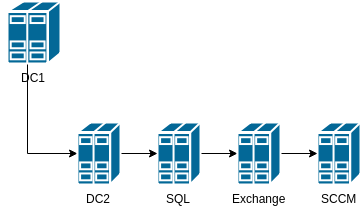
\includegraphics[width=8cm]{Netwerkdiagram.png}
\end{center}

\section{Server Requirements}

\begin{enumerate}
\item DC1
    \begin{enumerate}
    \item RAM: 2048 MB
    \item HDD: 50 GB
    \item Netwerkadapters: NAT en Internal Network (jenduf.gent)
            \begin{enumerate}
            \item NAT
            \end{enumerate}
            \begin{enumerate}
            \item IP: 192.168.1.1
            \item SN: 255.255.255.0
            \end{enumerate}
    \item OS Version: Windows Server 2016 
    \end{enumerate}
    
\clearpage

\item DC2
    \begin{enumerate}
    \item RAM: 2048 MB
    \item HDD: 50 GB
    \item Netwerkadapters: Internal Network (jenduf.gent)
            \begin{enumerate}
            \item IP: 192.168.1.2
            \item SN: 255.255.255.0
            \item DG: 192.168.1.1
            \end{enumerate}
    \item OS Version: Windows Server 2016 
    \end{enumerate}
    
\item SQL Server
    \begin{enumerate}
    \item RAM: 2048 MB
    \item HDD: 50 GB
    \item Netwerkadapters: Internal Network (jenduf.gent)
            \begin{enumerate}
            \item IP: 192.168.1.3
            \item SN: 255.255.255.0
            \item DG: 192.168.1.1
            \end{enumerate}
    \item OS Version: Windows Server 2016
    \item SQL Version: SQL Server 2013-2016
    \end{enumerate}
\item Exchange Server
    \begin{enumerate}
    \item RAM: 8096 MB
    \item HDD: 100 GB
    \item Netwerkadapters: Internal Network (jenduf.gent)
            \begin{enumerate}
            \item IP: 192.168.1.4
            \item SN: 255.255.255.0
            \item DG: 192.168.1.1
            \end{enumerate}
    \item OS Version: Windows Server 2016
    \item Exchange Version: Exchange Server 2013-2016
    \end{enumerate}
\item SCCM Server
    \begin{enumerate}
    \item RAM: 8089 MB
    \item HDD: 100 GB
    \item Netwerkadapters: Internal Network (jenduf.gent)
            \begin{enumerate}
            \item IP: 192.168.1.5
            \item SN: 255.255.255.0
            \item DG: 192.168.1.1
            \end{enumerate}
    \item OS Version: Windows Server 2016
    \item OS Version: Windows Deployment Server 2012
    \end{enumerate}
\end{enumerate}

\section{Windows Server Installatie}
\begin{center}
	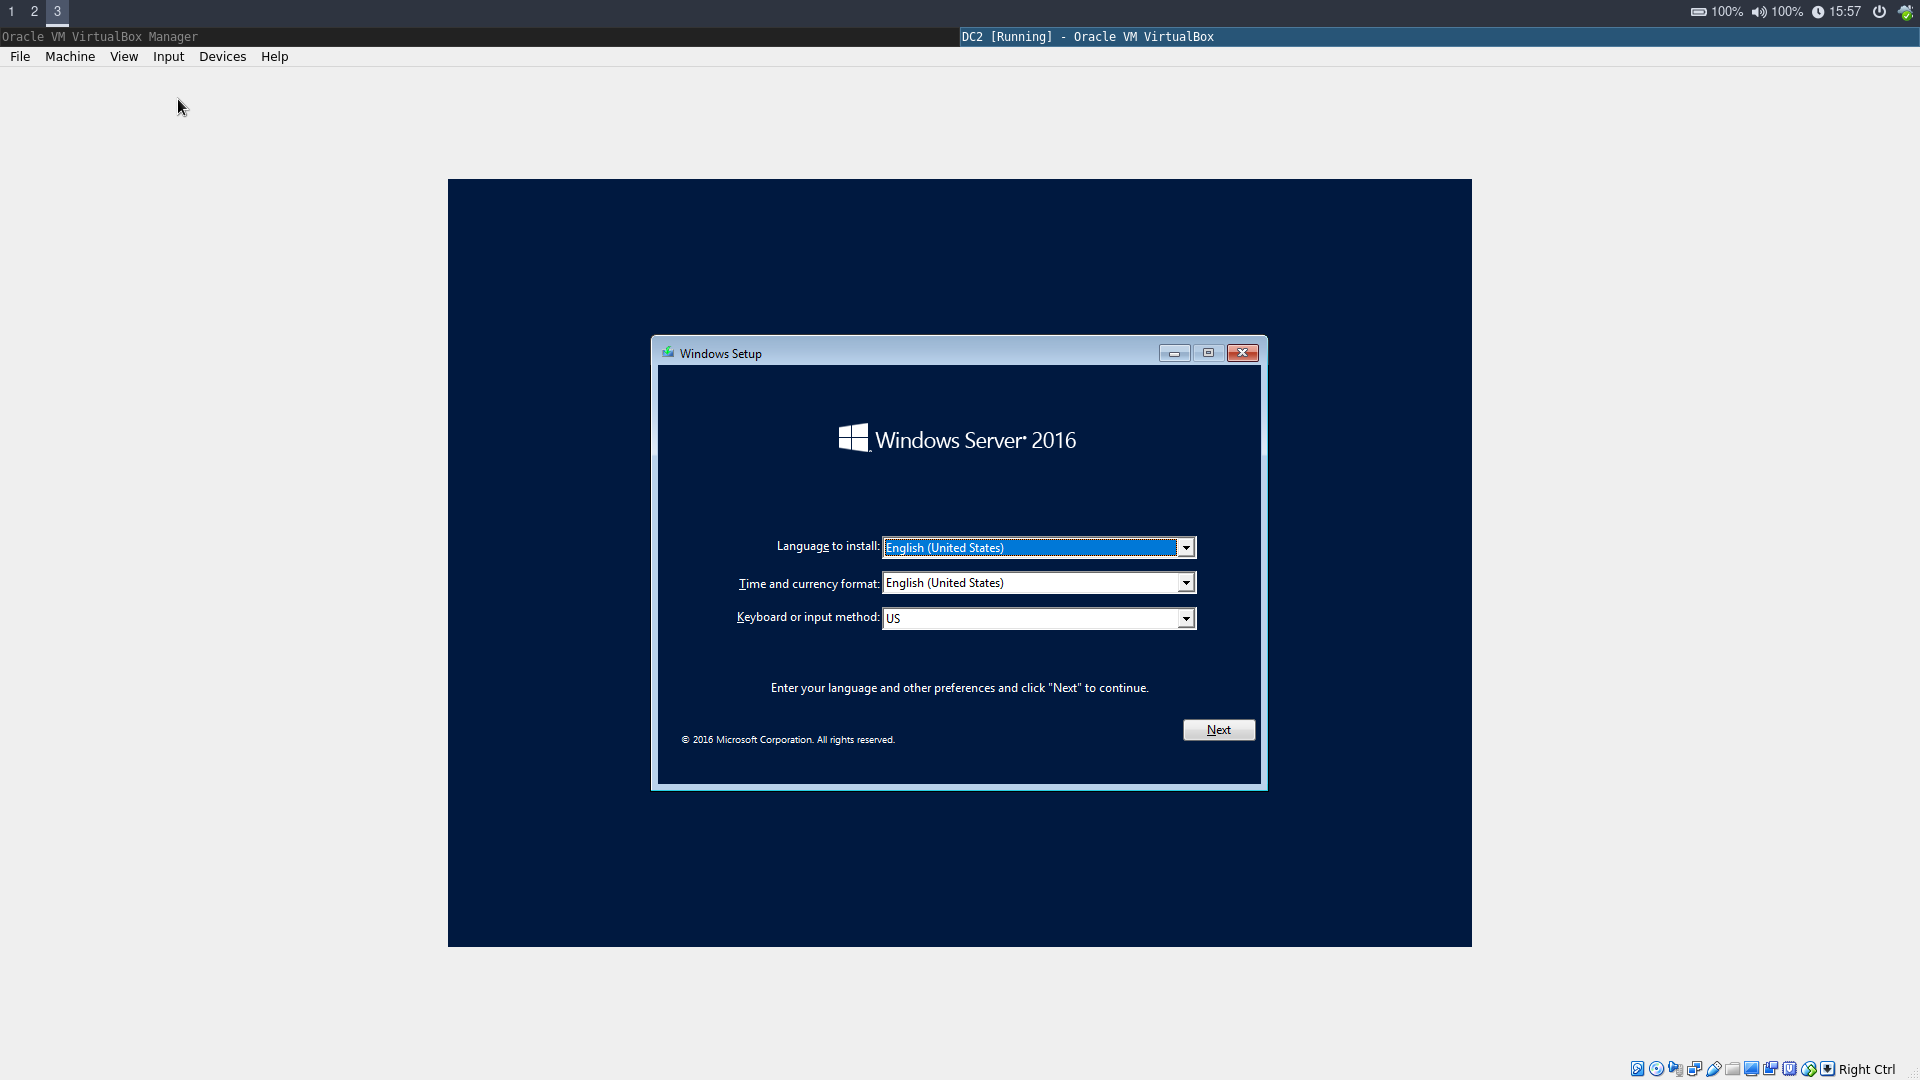
\includegraphics[width=15cm]{Pictures/Windows_Install/1542293852.png}
	Selecteer de gewenste taalinstellingen.
\end{center}
\begin{center}
	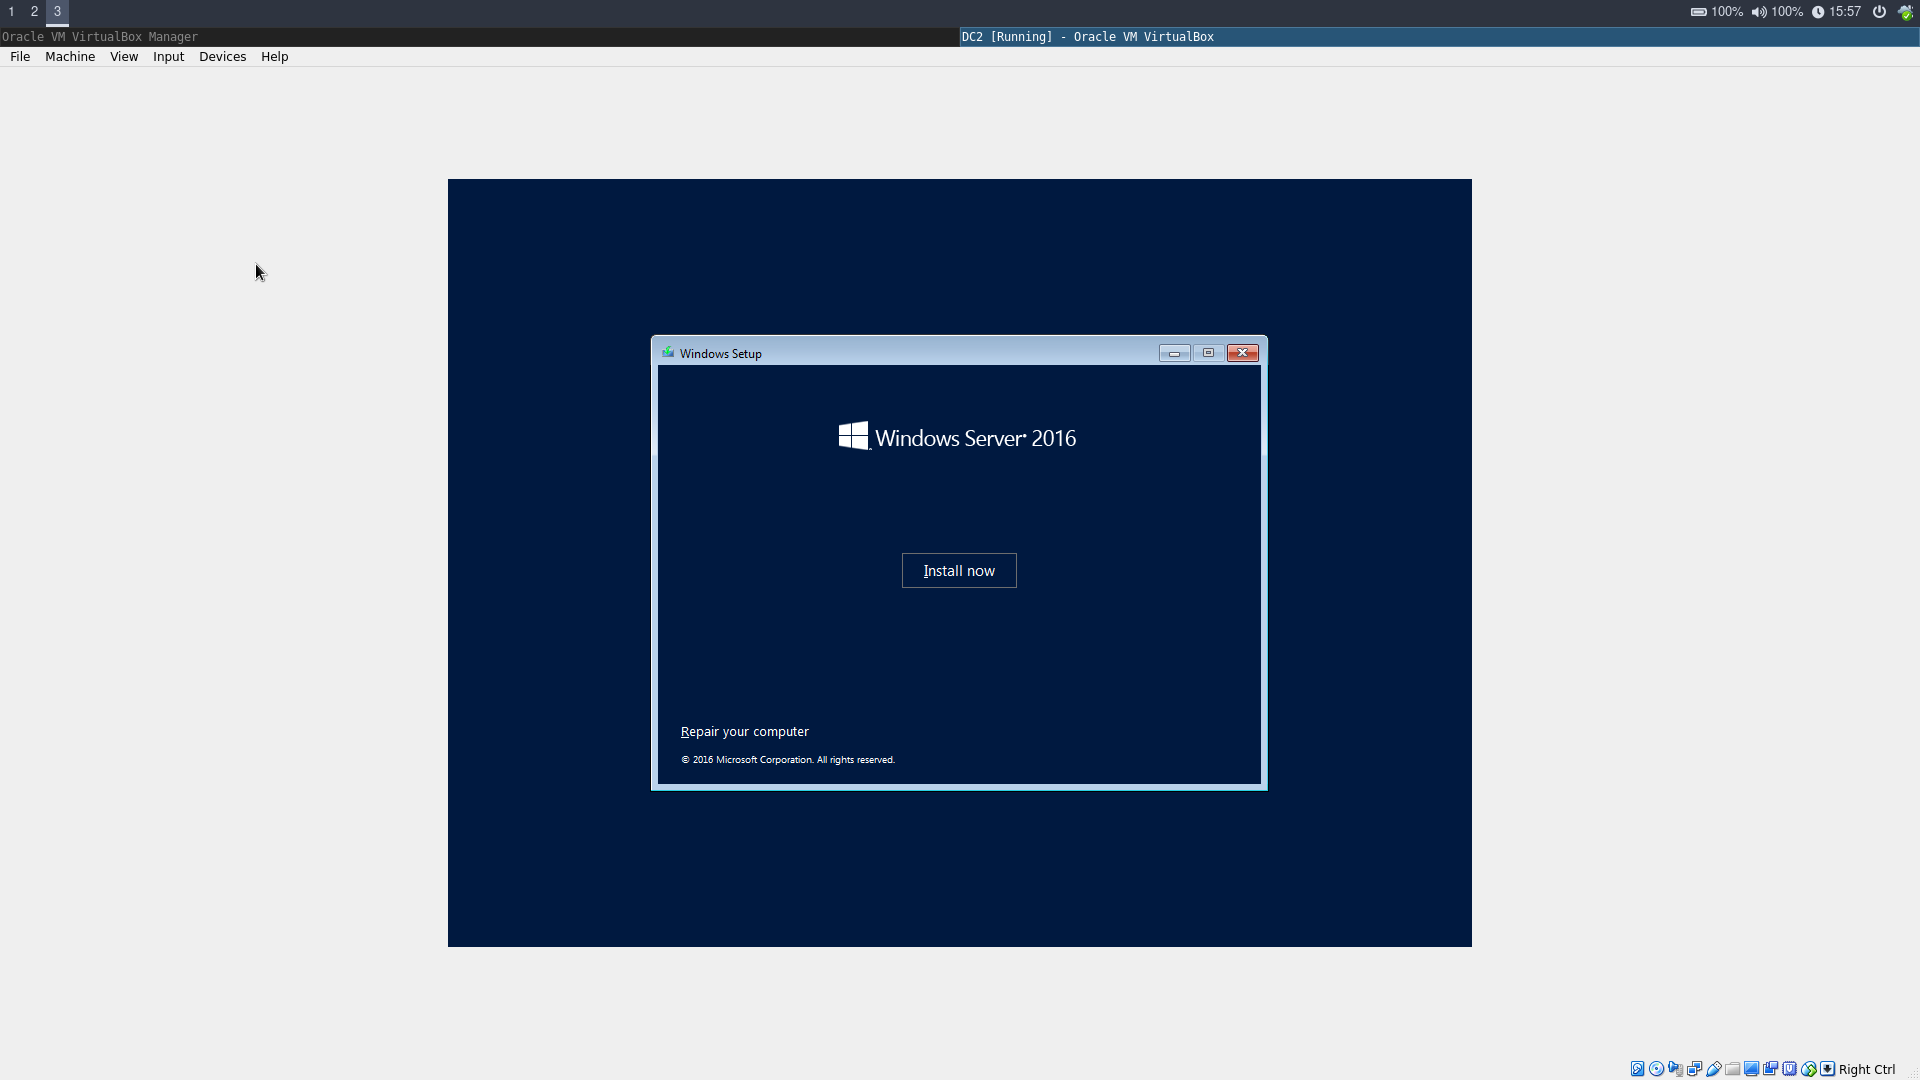
\includegraphics[width=15cm]{Pictures/Windows_Install/1542293872.png}
	
	Start de installatie.
\end{center}
\begin{center}
	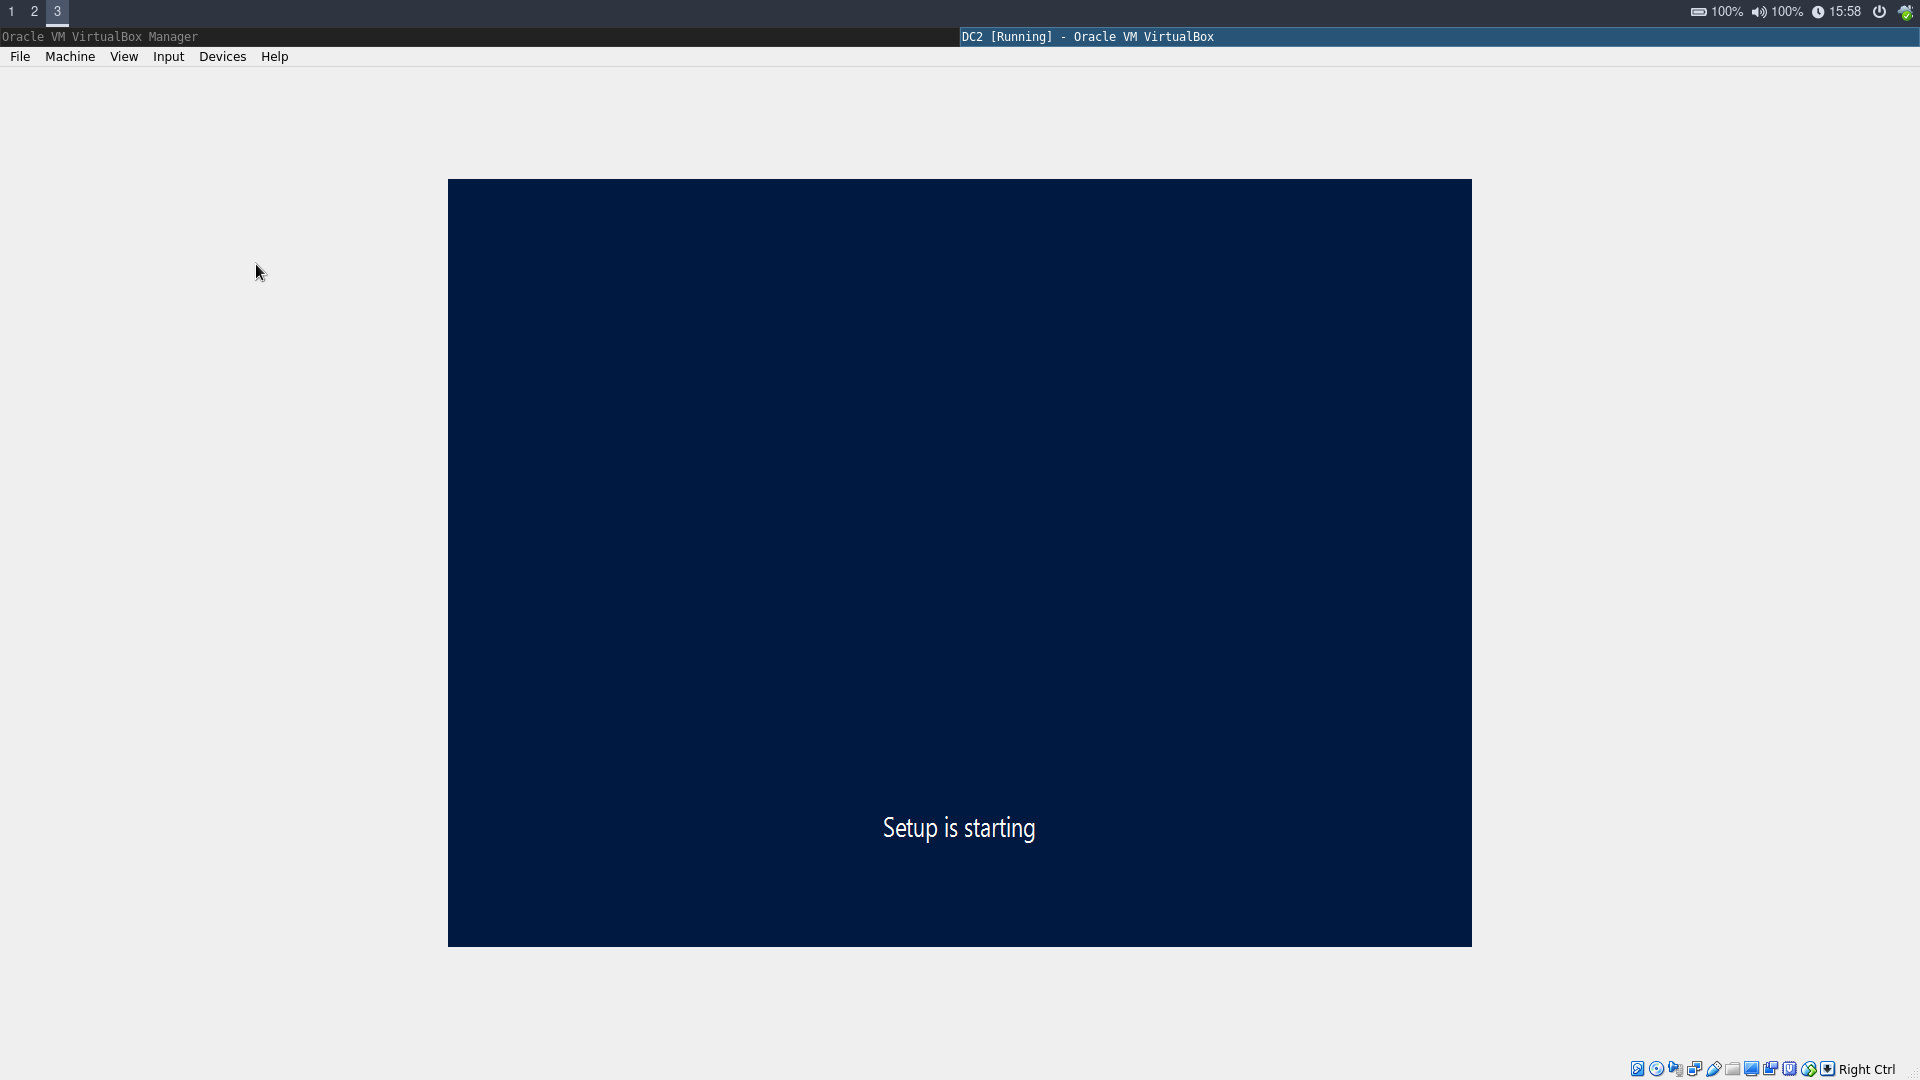
\includegraphics[width=15cm]{Pictures/Windows_Install/1542293887.png}
\end{center}
\begin{center}
	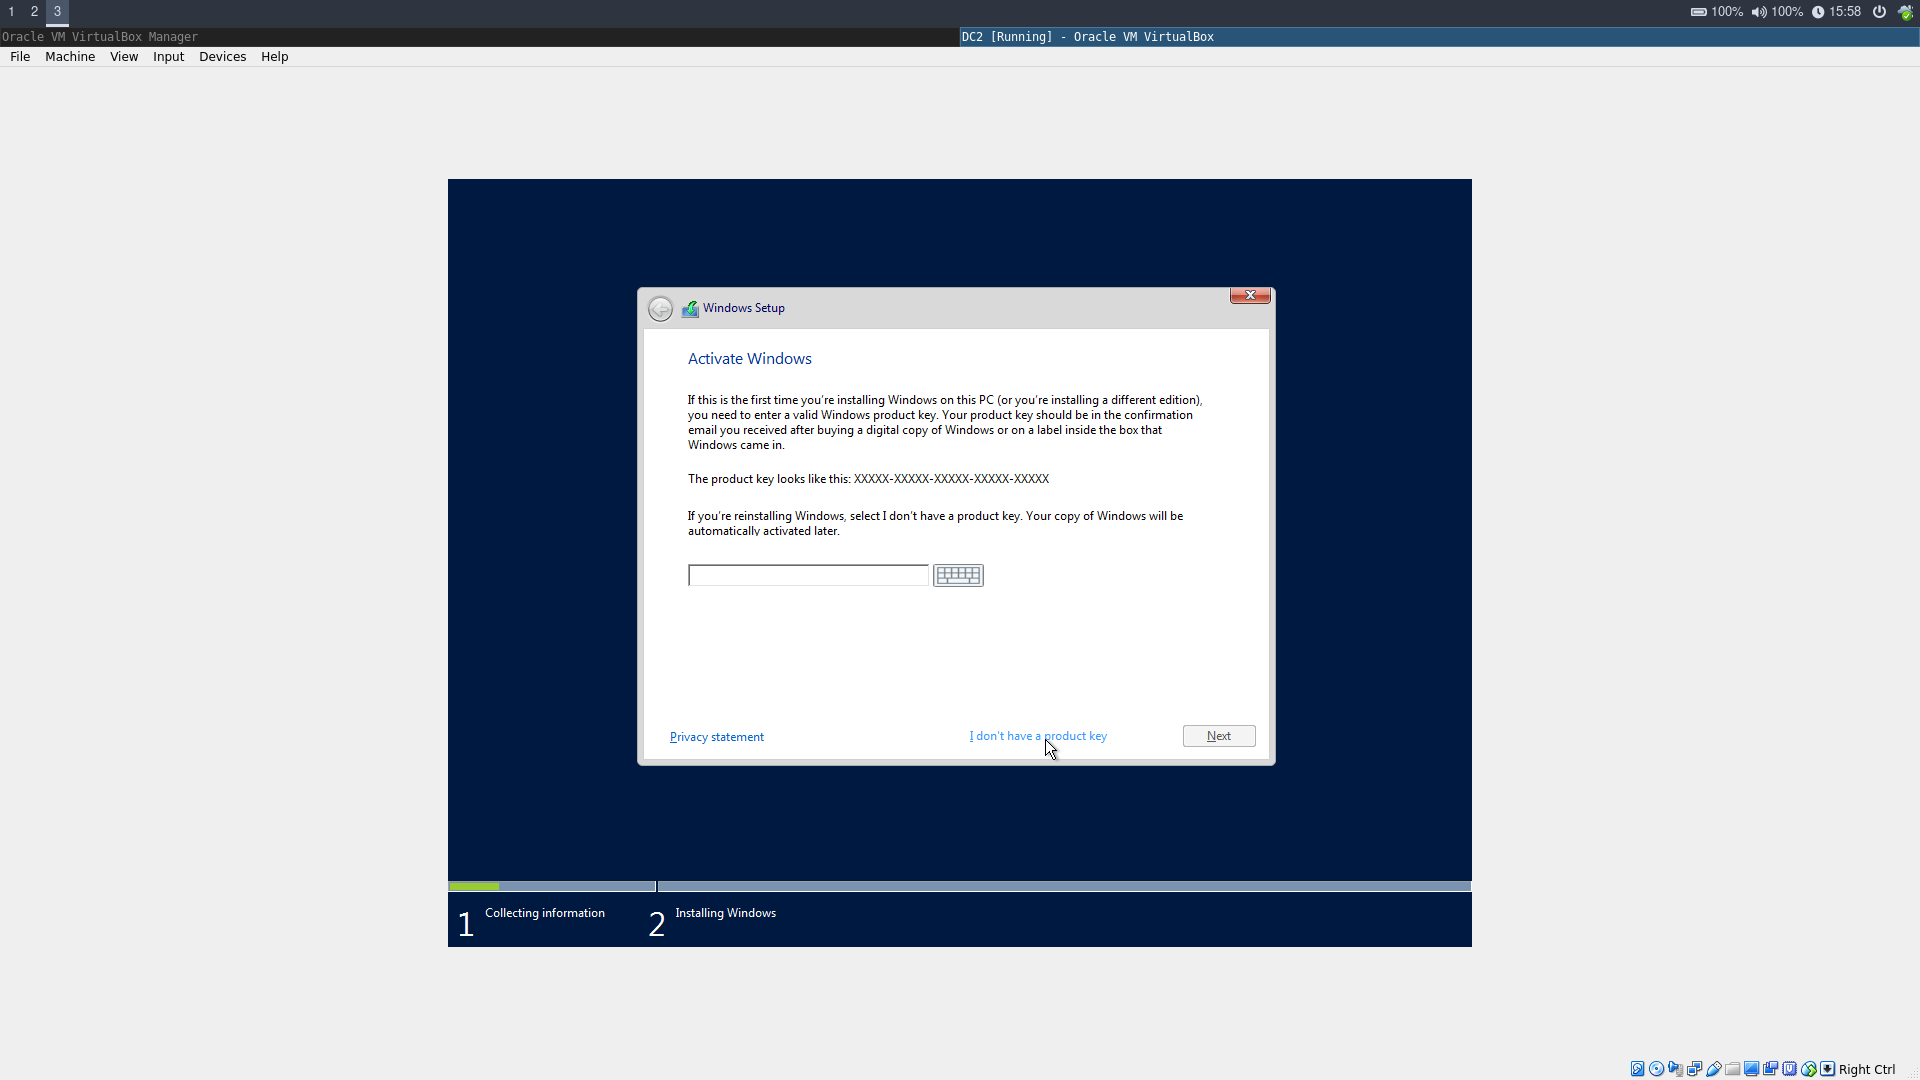
\includegraphics[width=15cm]{Pictures/Windows_Install/1542293899.png}
	
	Selecteer "I don't have a product key".
\end{center}
\begin{center}
	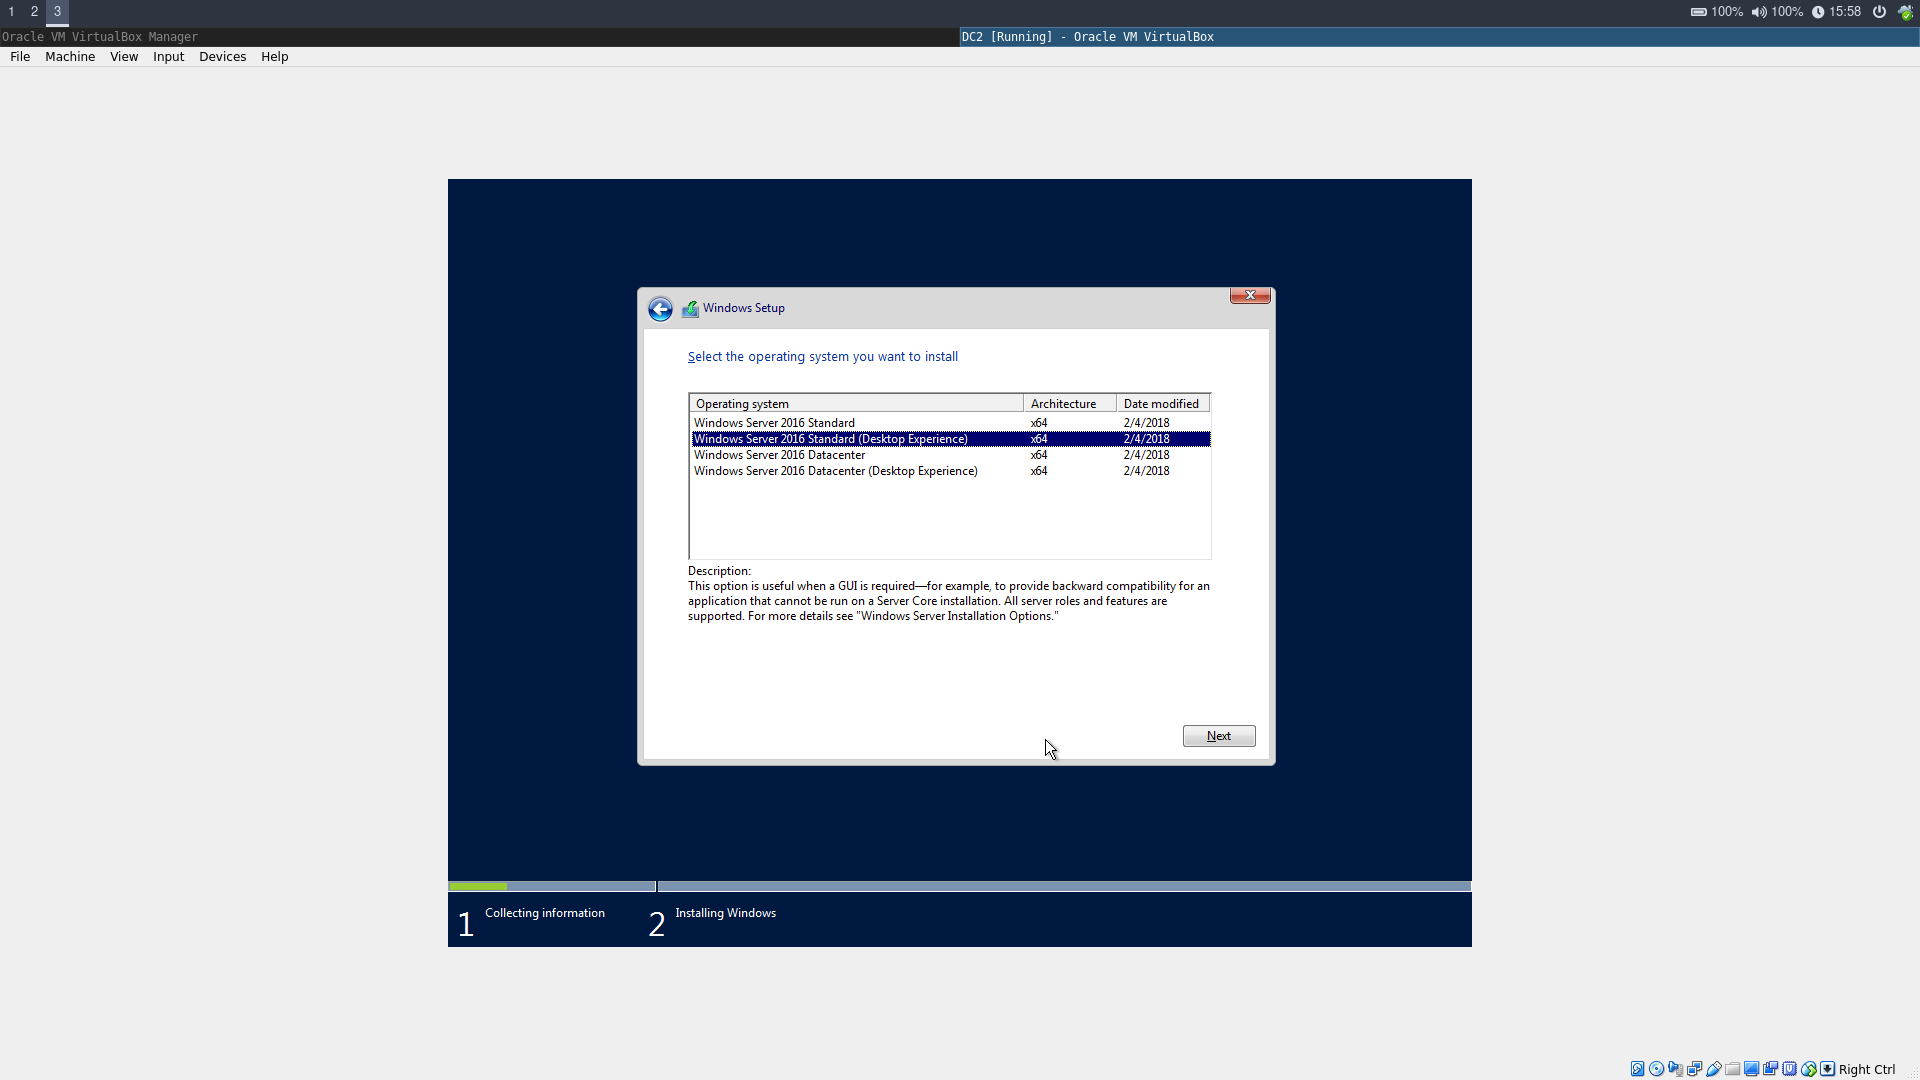
\includegraphics[width=15cm]{Pictures/Windows_Install/1542293908.png}
	
	Selecteer "Windows Server 2016 Standard (Desktop Experience)".
\end{center}
\begin{center}
	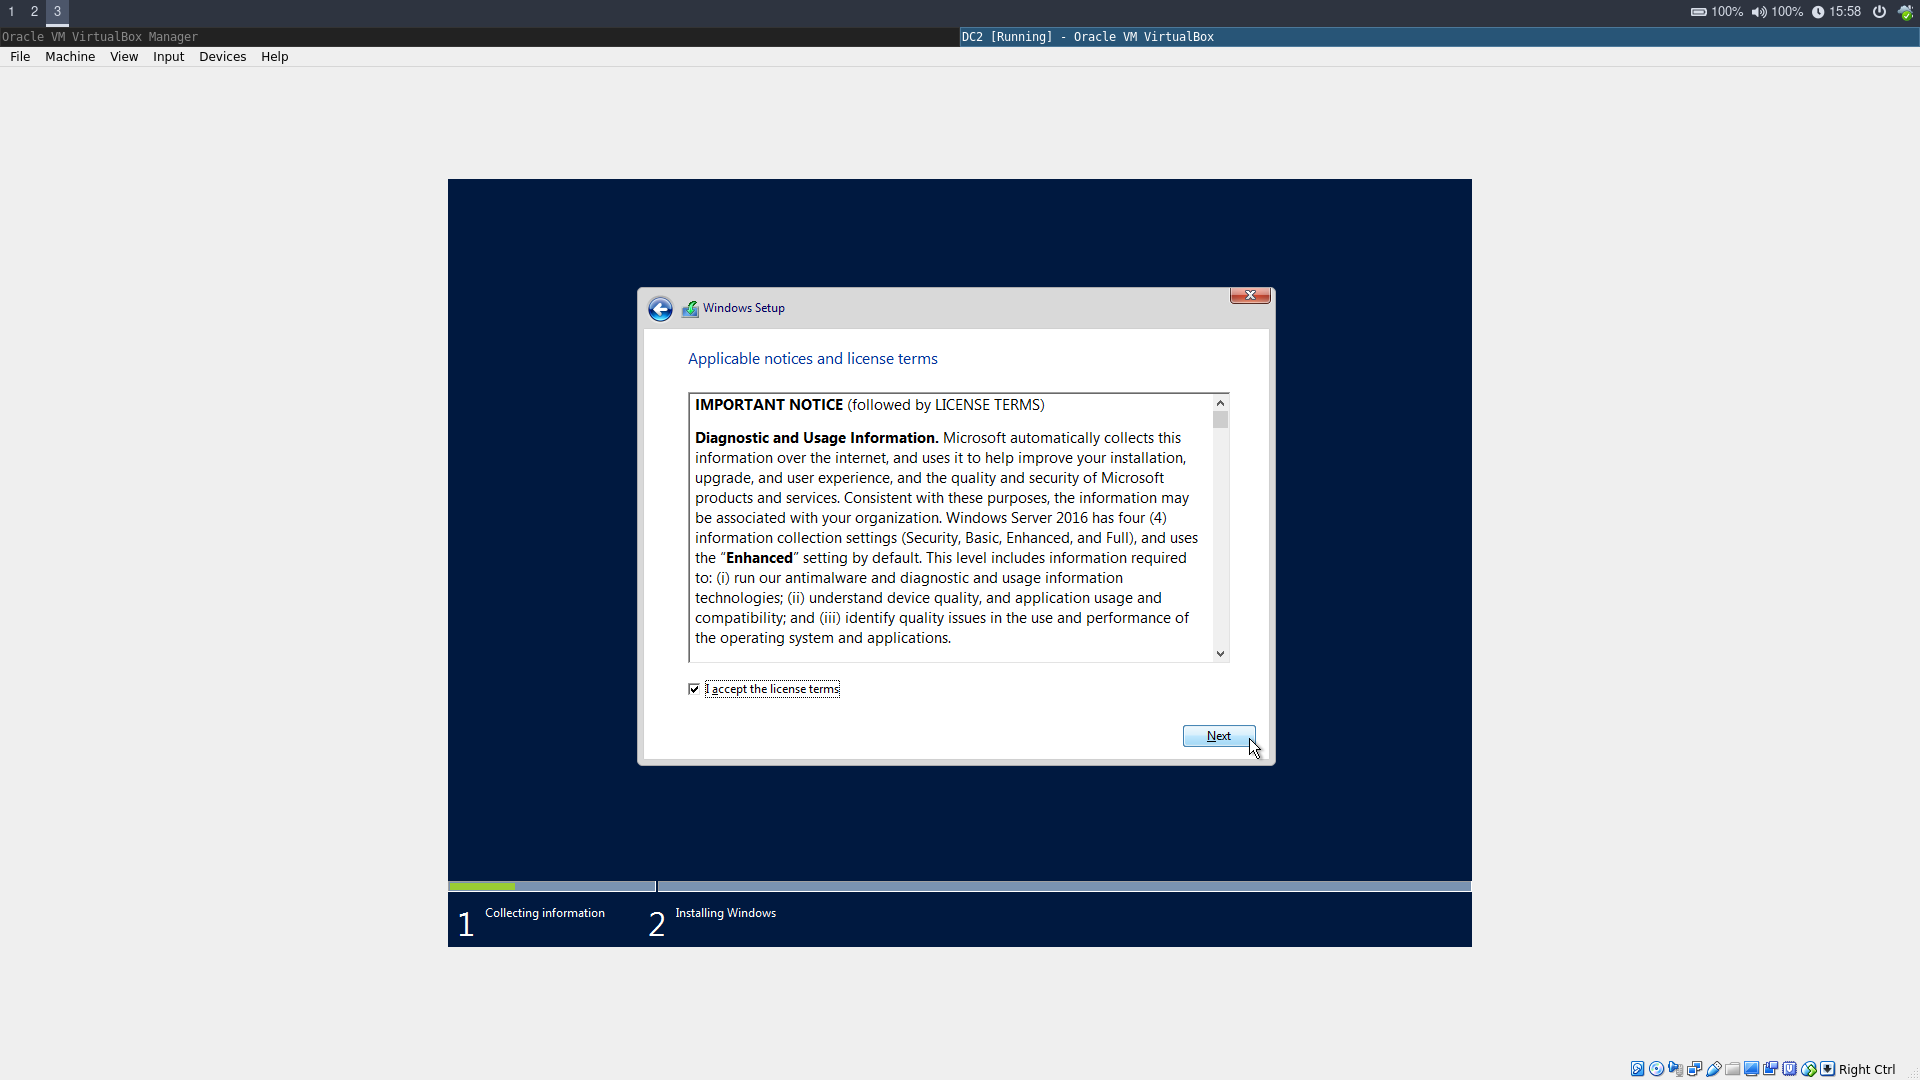
\includegraphics[width=15cm]{Pictures/Windows_Install/1542293921.png}
	
	Ga akkoord met de gebruiksvoorwaarden.
\end{center}
\begin{center}
	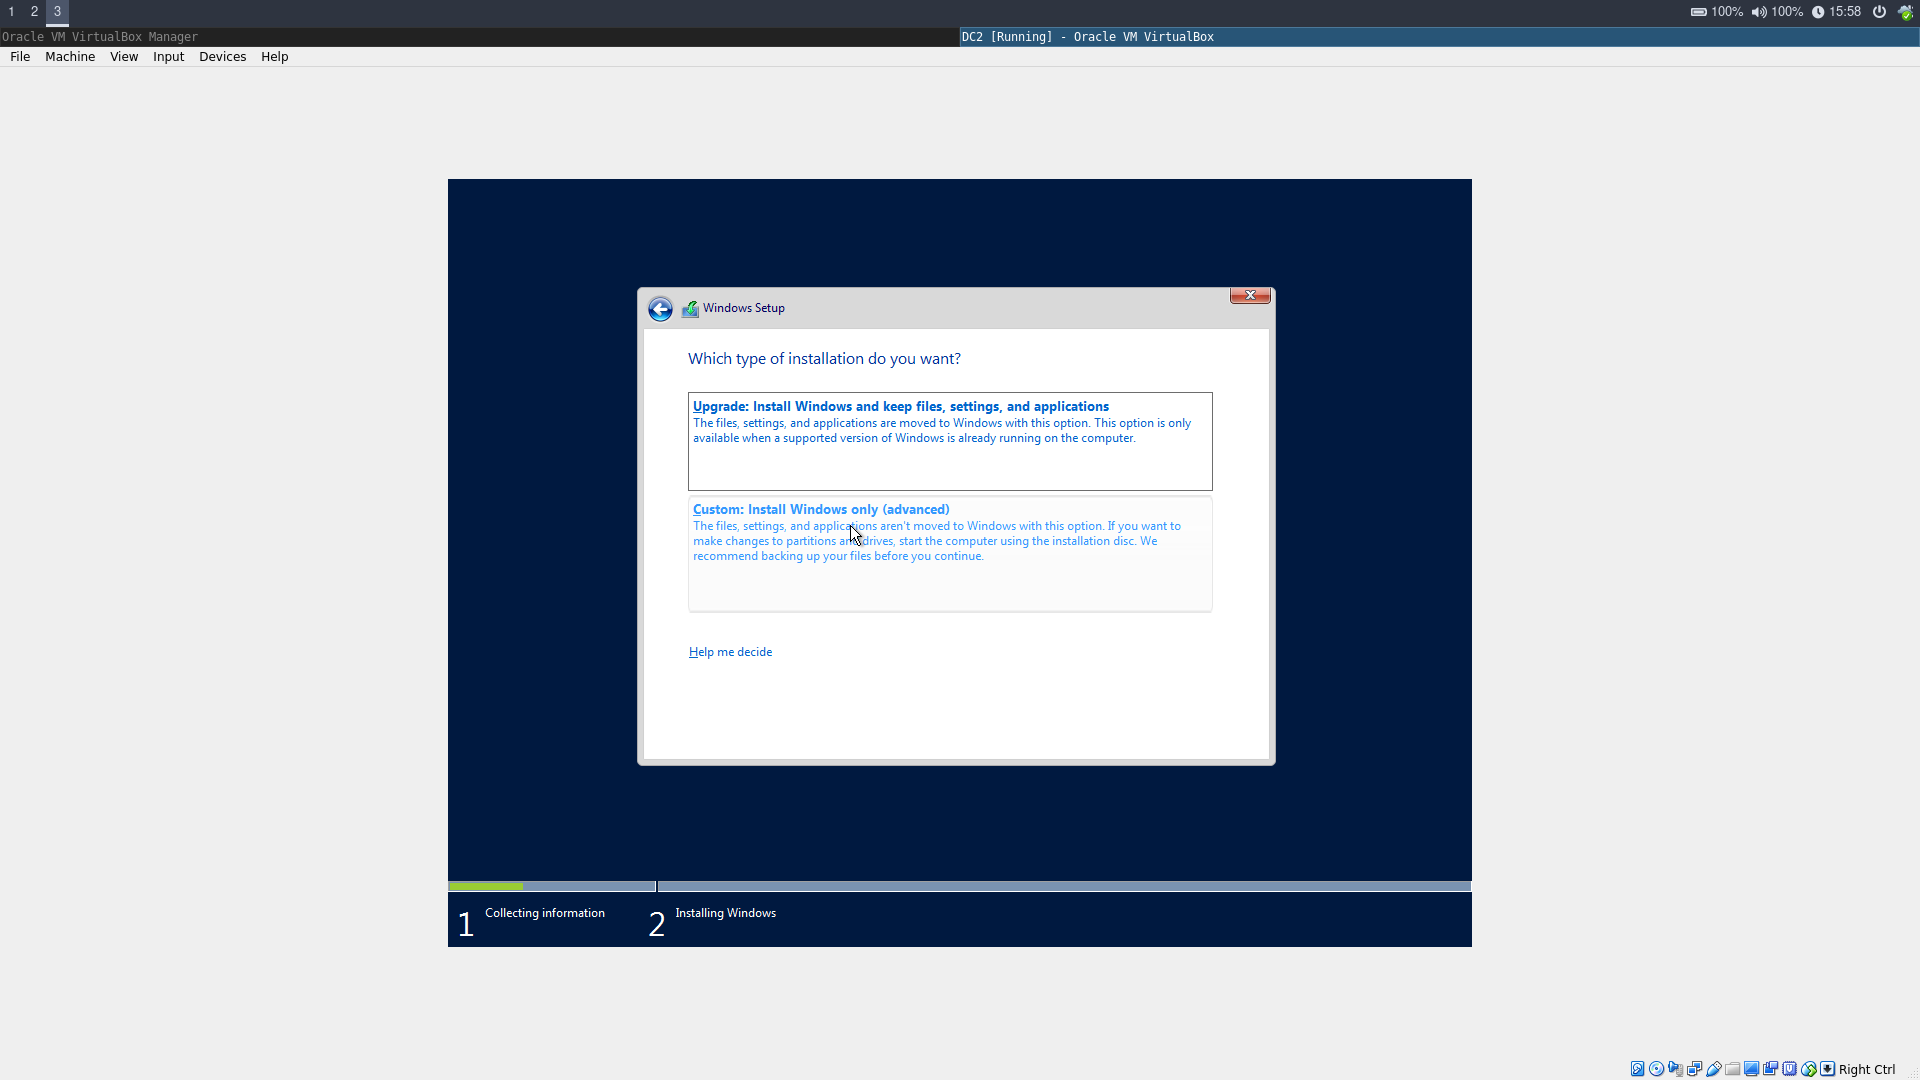
\includegraphics[width=15cm]{Pictures/Windows_Install/1542293929.png}
	
	Selecteer "Costum: Install Windows only (Advanced)".
\end{center}
\begin{center}
	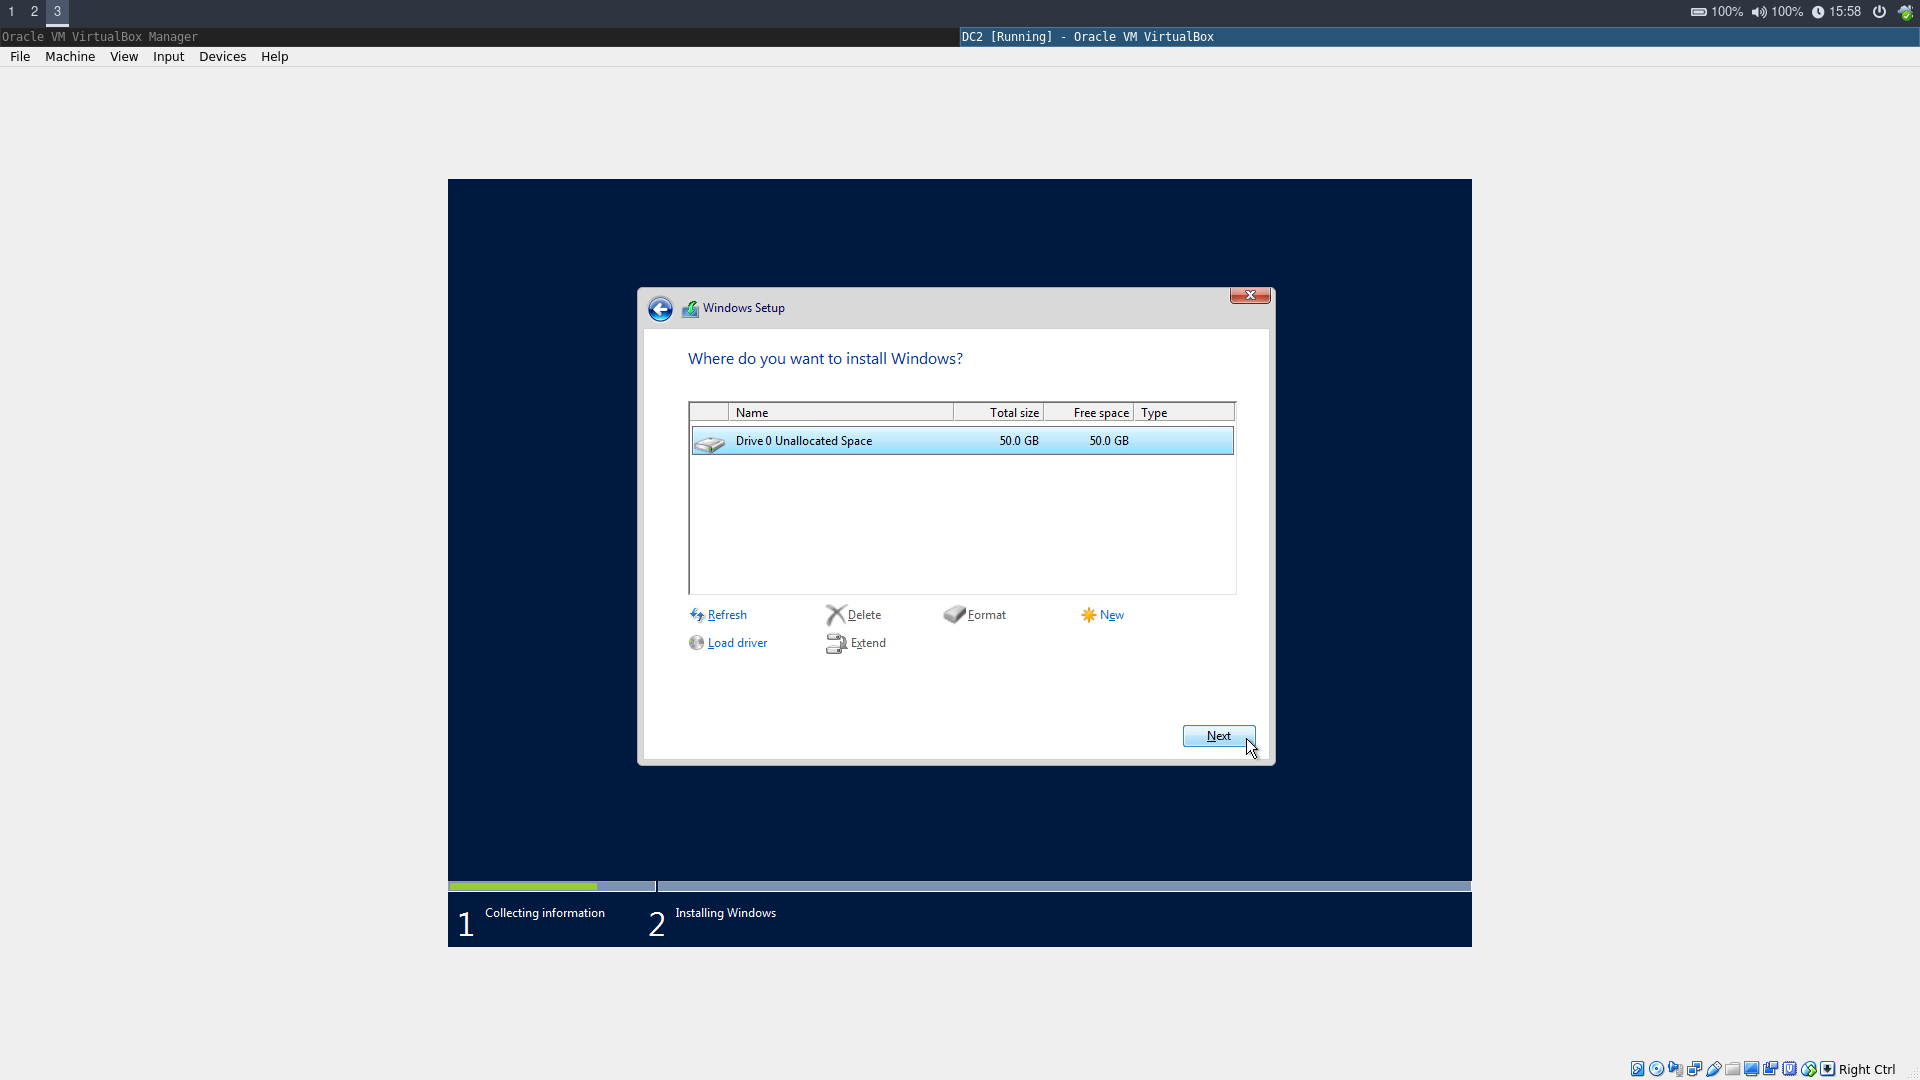
\includegraphics[width=15cm]{Pictures/Windows_Install/1542293934.png}
	
	Ga verder.
\end{center}
\begin{center}
	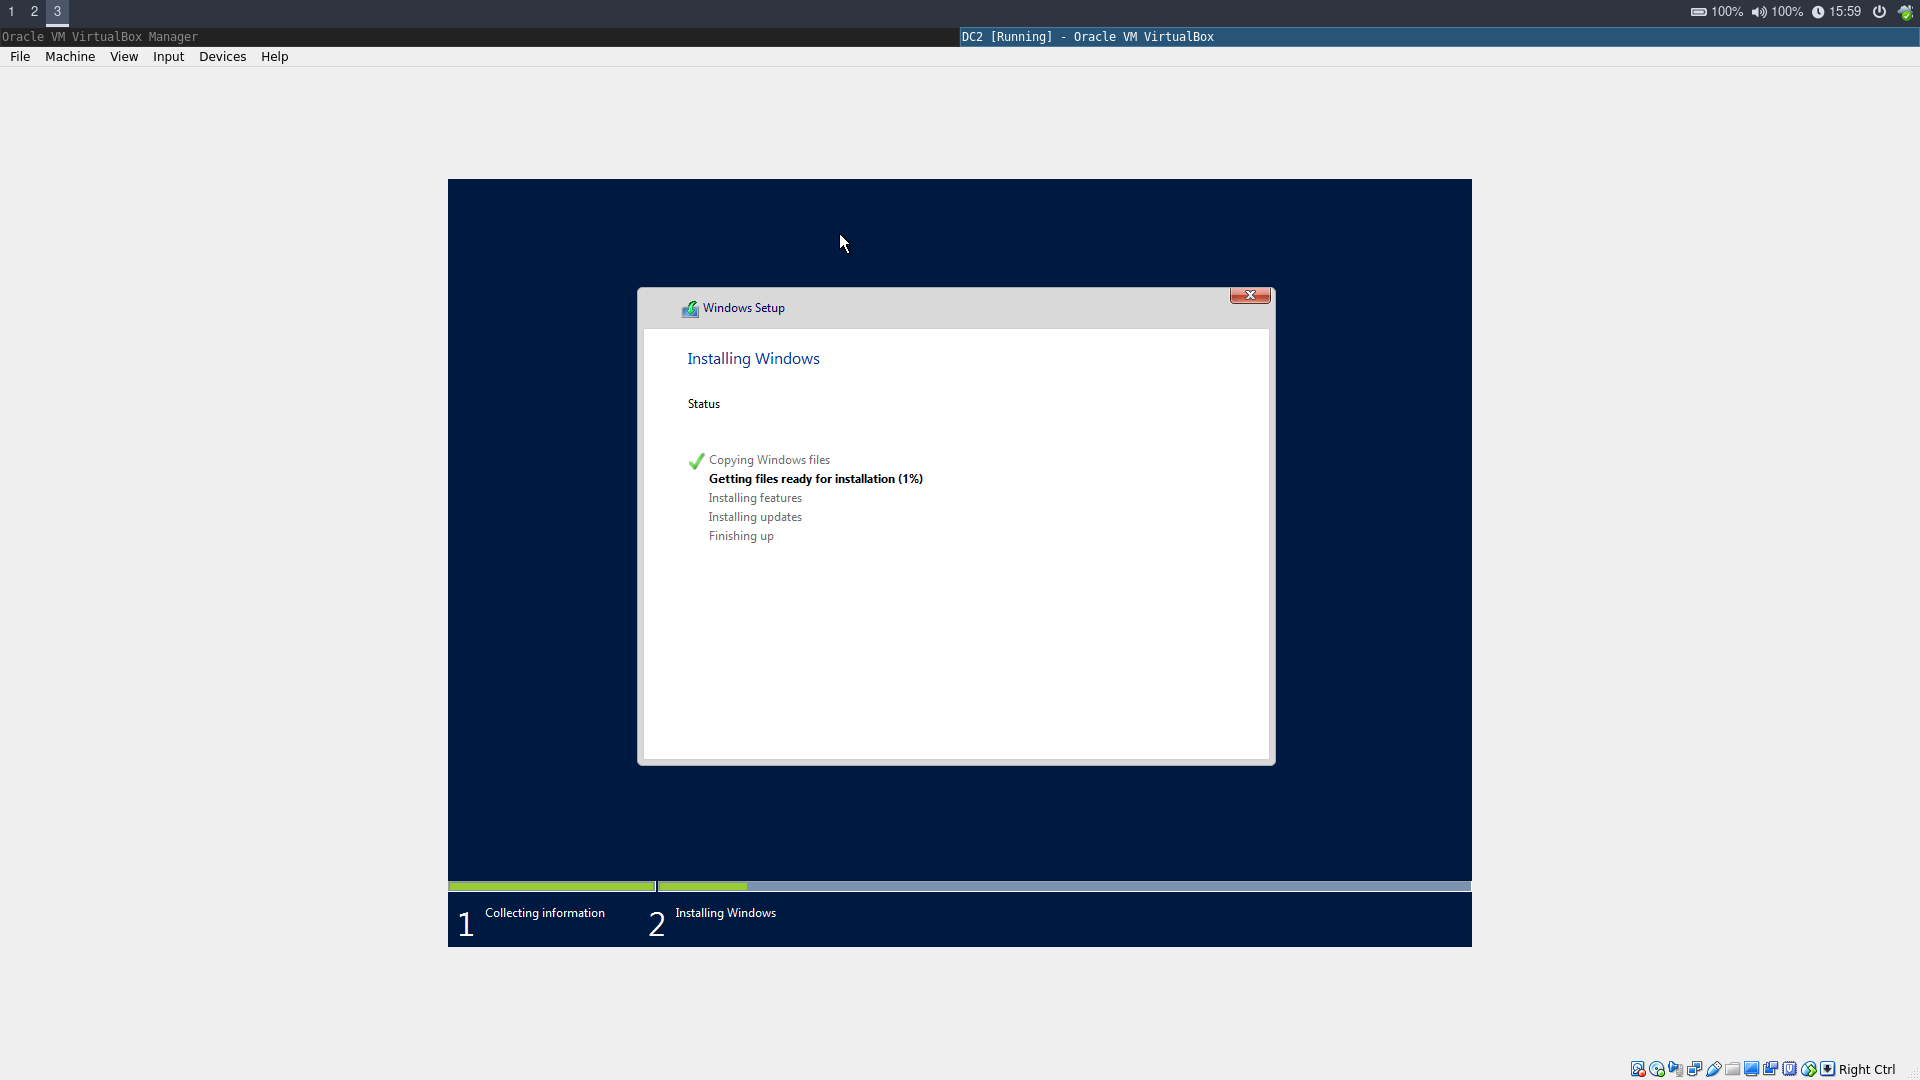
\includegraphics[width=15cm]{Pictures/Windows_Install/1542293945.png}
\end{center}
\subsection{Server Hernoemen}
\begin{center}
	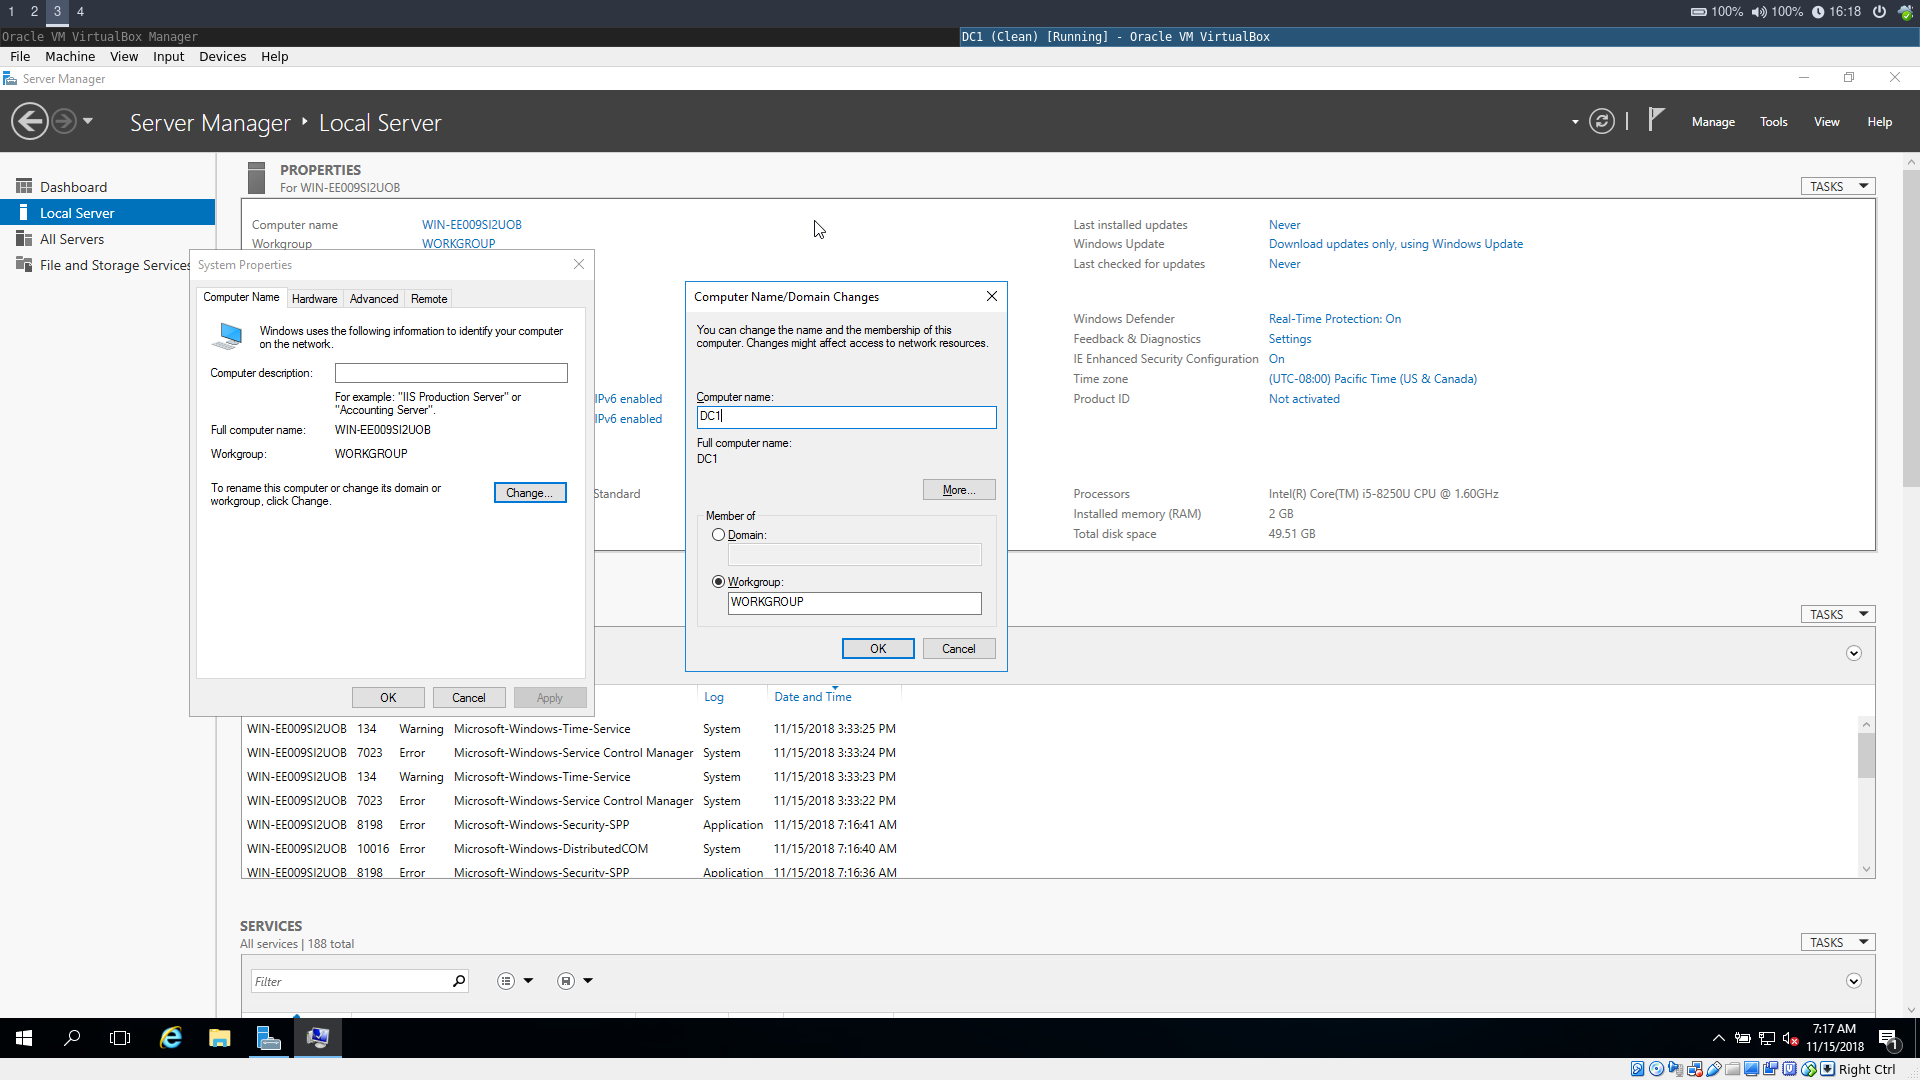
\includegraphics[width=15cm]{Pictures/DC1/Basisconfiguratie/1542295124.png}
\end{center}
\subsection{IP Instellingen}
\begin{center}
	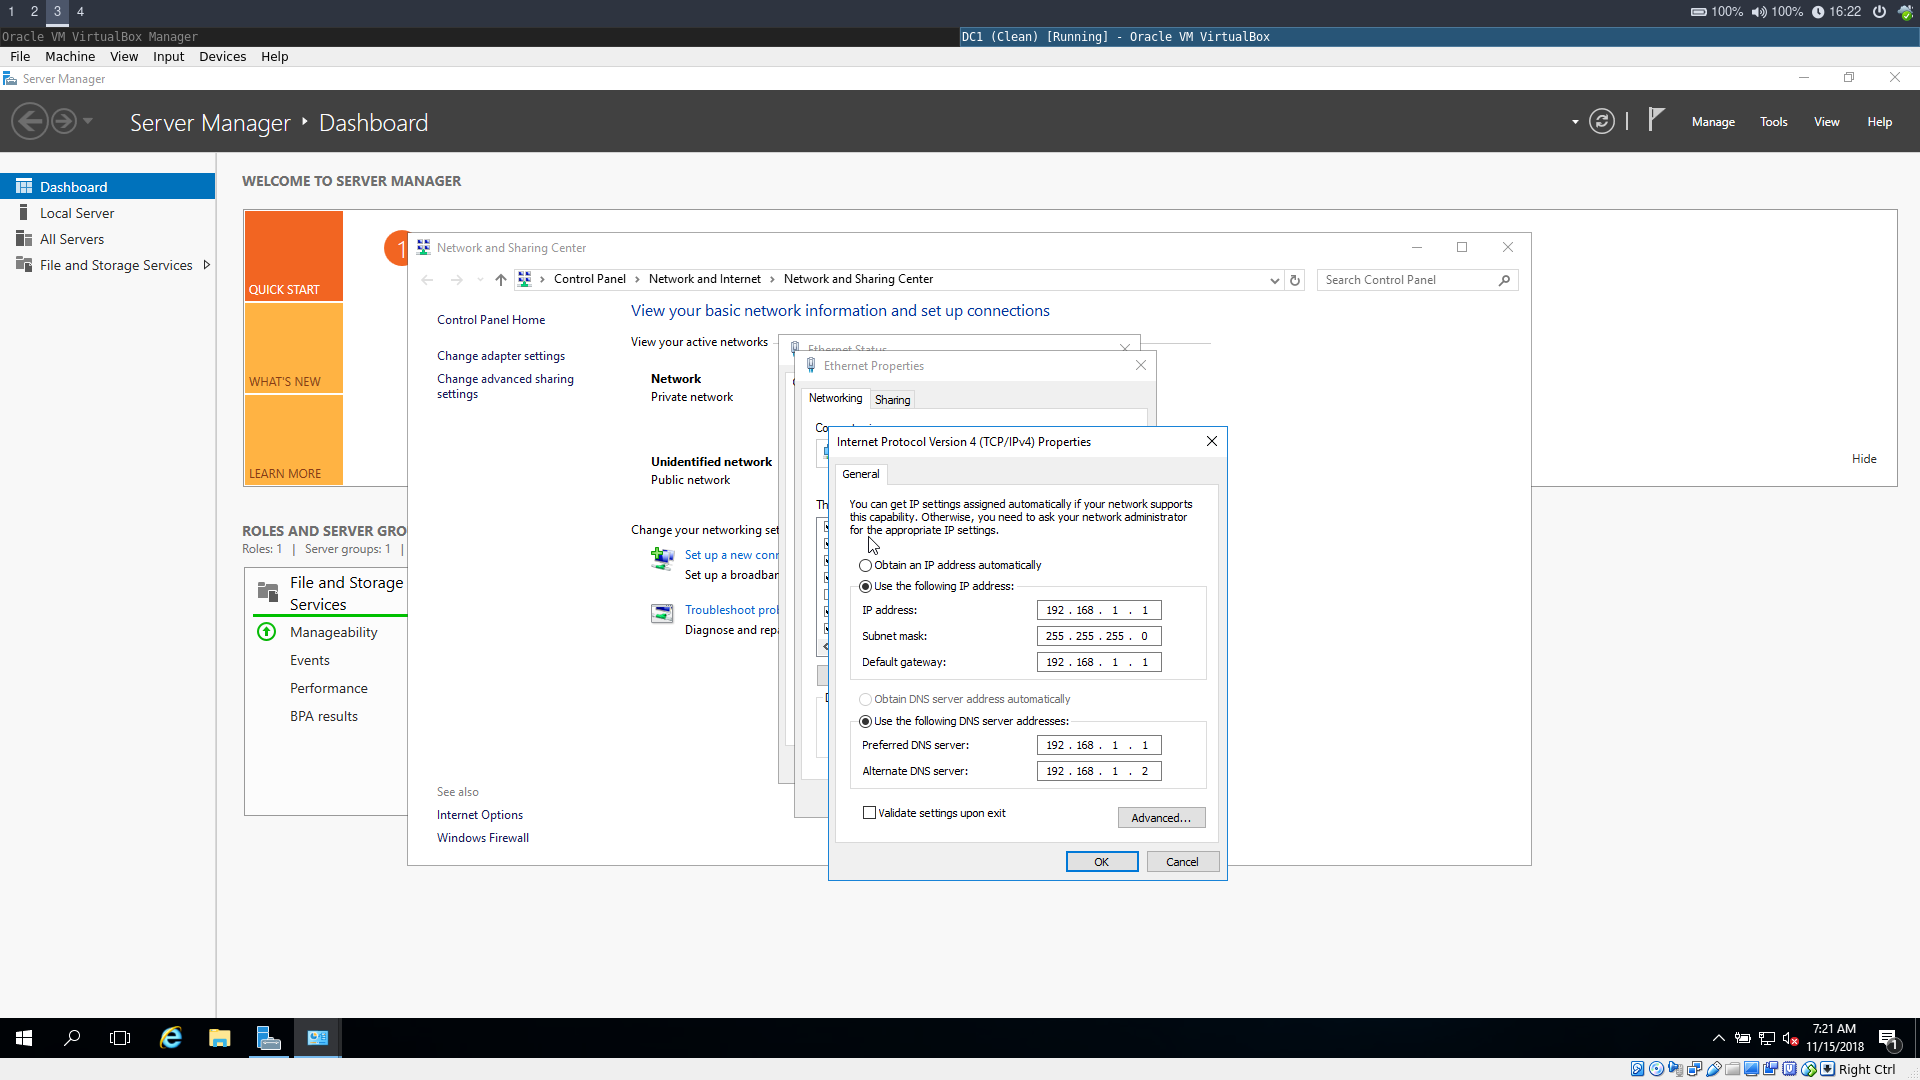
\includegraphics[width=15cm]{Pictures/DC1/Basisconfiguratie/1542295346.png}
\end{center}

\section{Installatie ADDS}
\begin{center}
	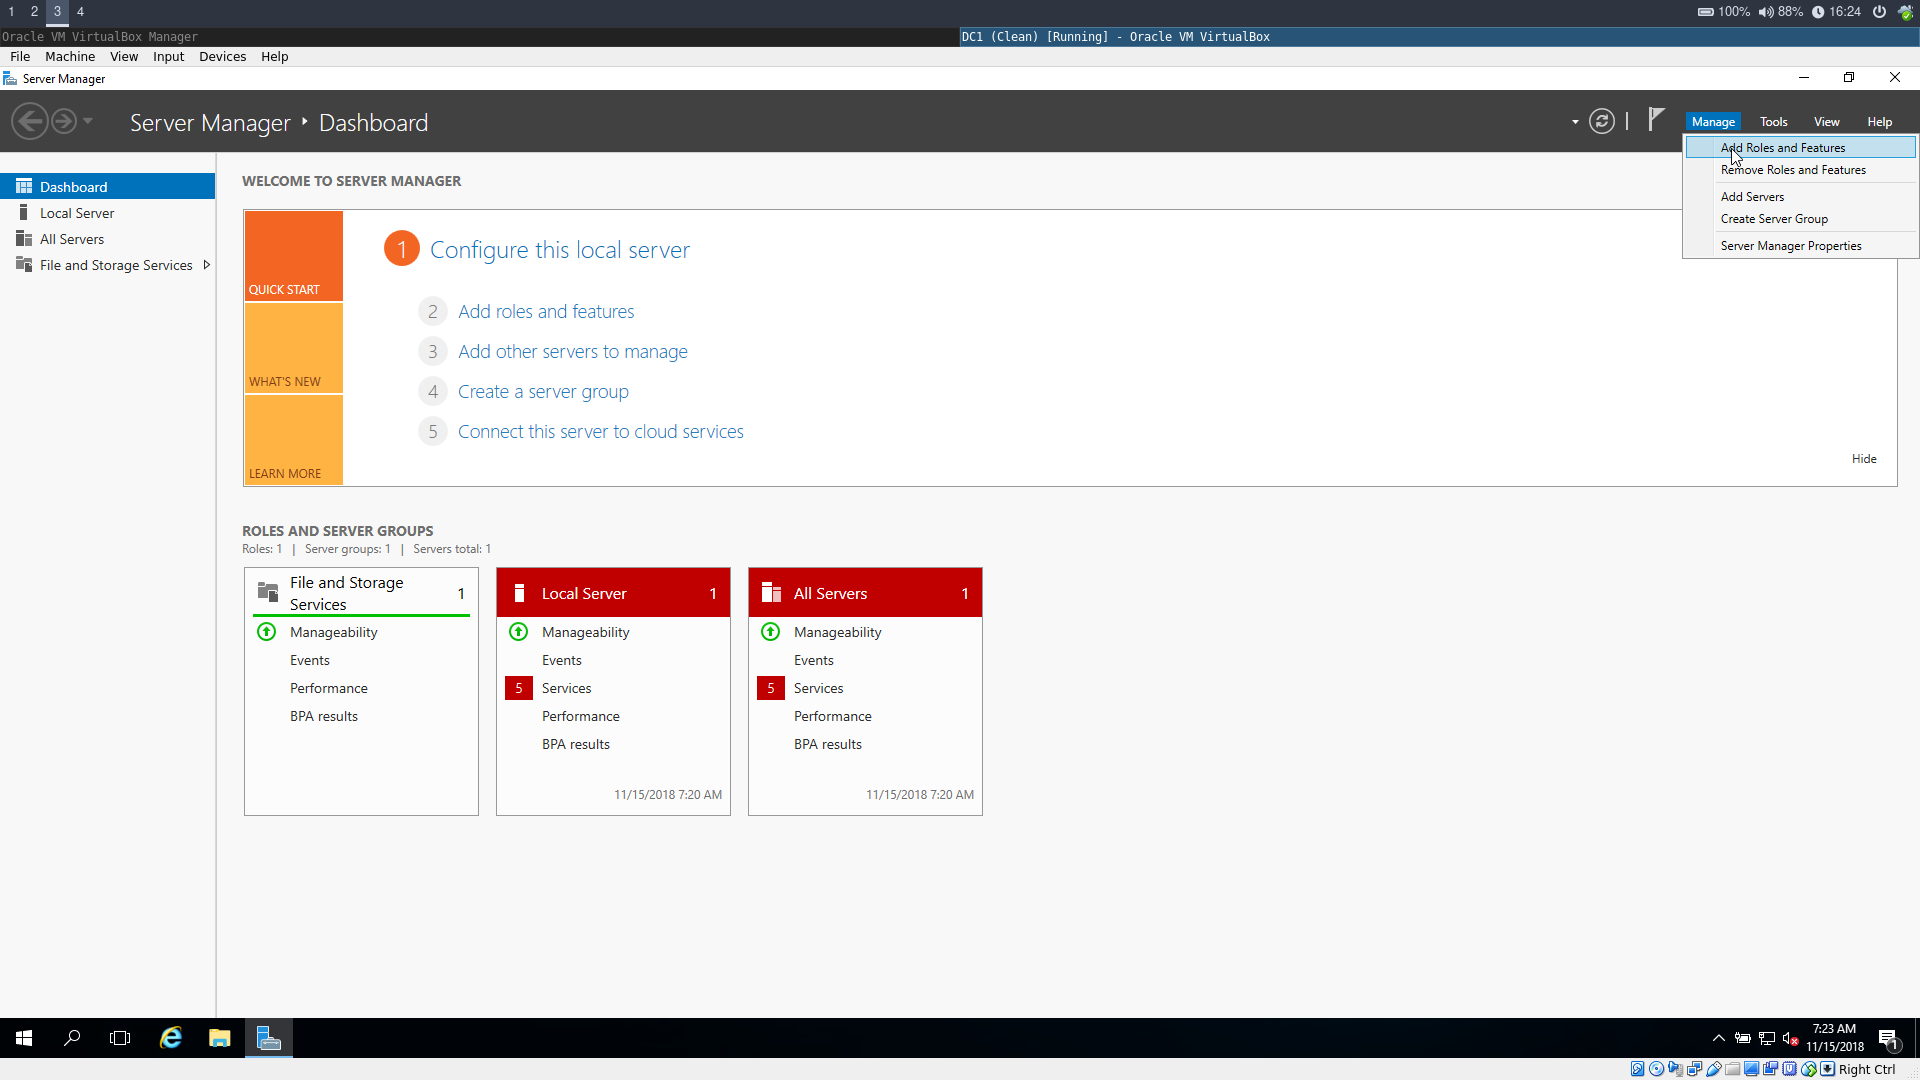
\includegraphics[width=15cm]{Pictures/DC1/ADDS/1542295445.png}
\end{center}
\begin{center}
	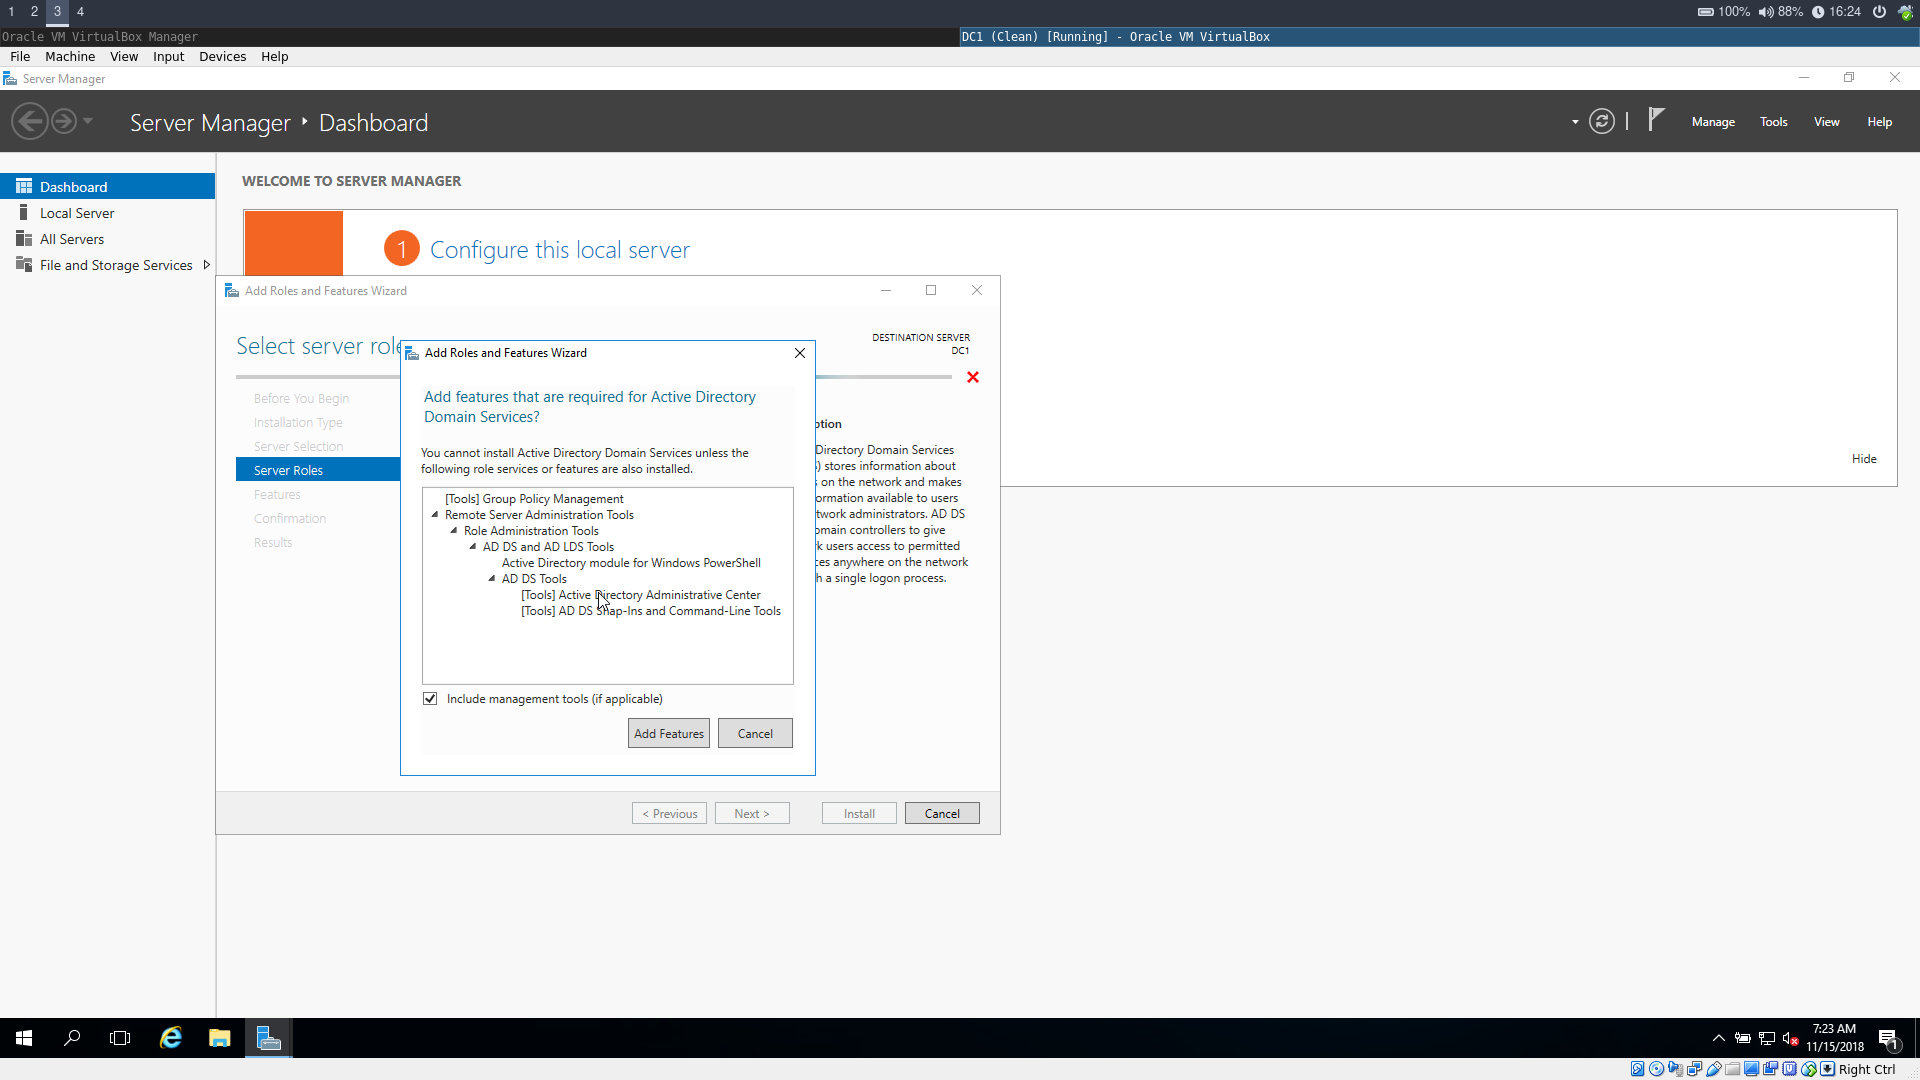
\includegraphics[width=15cm]{Pictures/DC1/ADDS/1542295457.png}
	
	Selecteer Active Directory Domain Service.
\end{center}
\begin{center}
	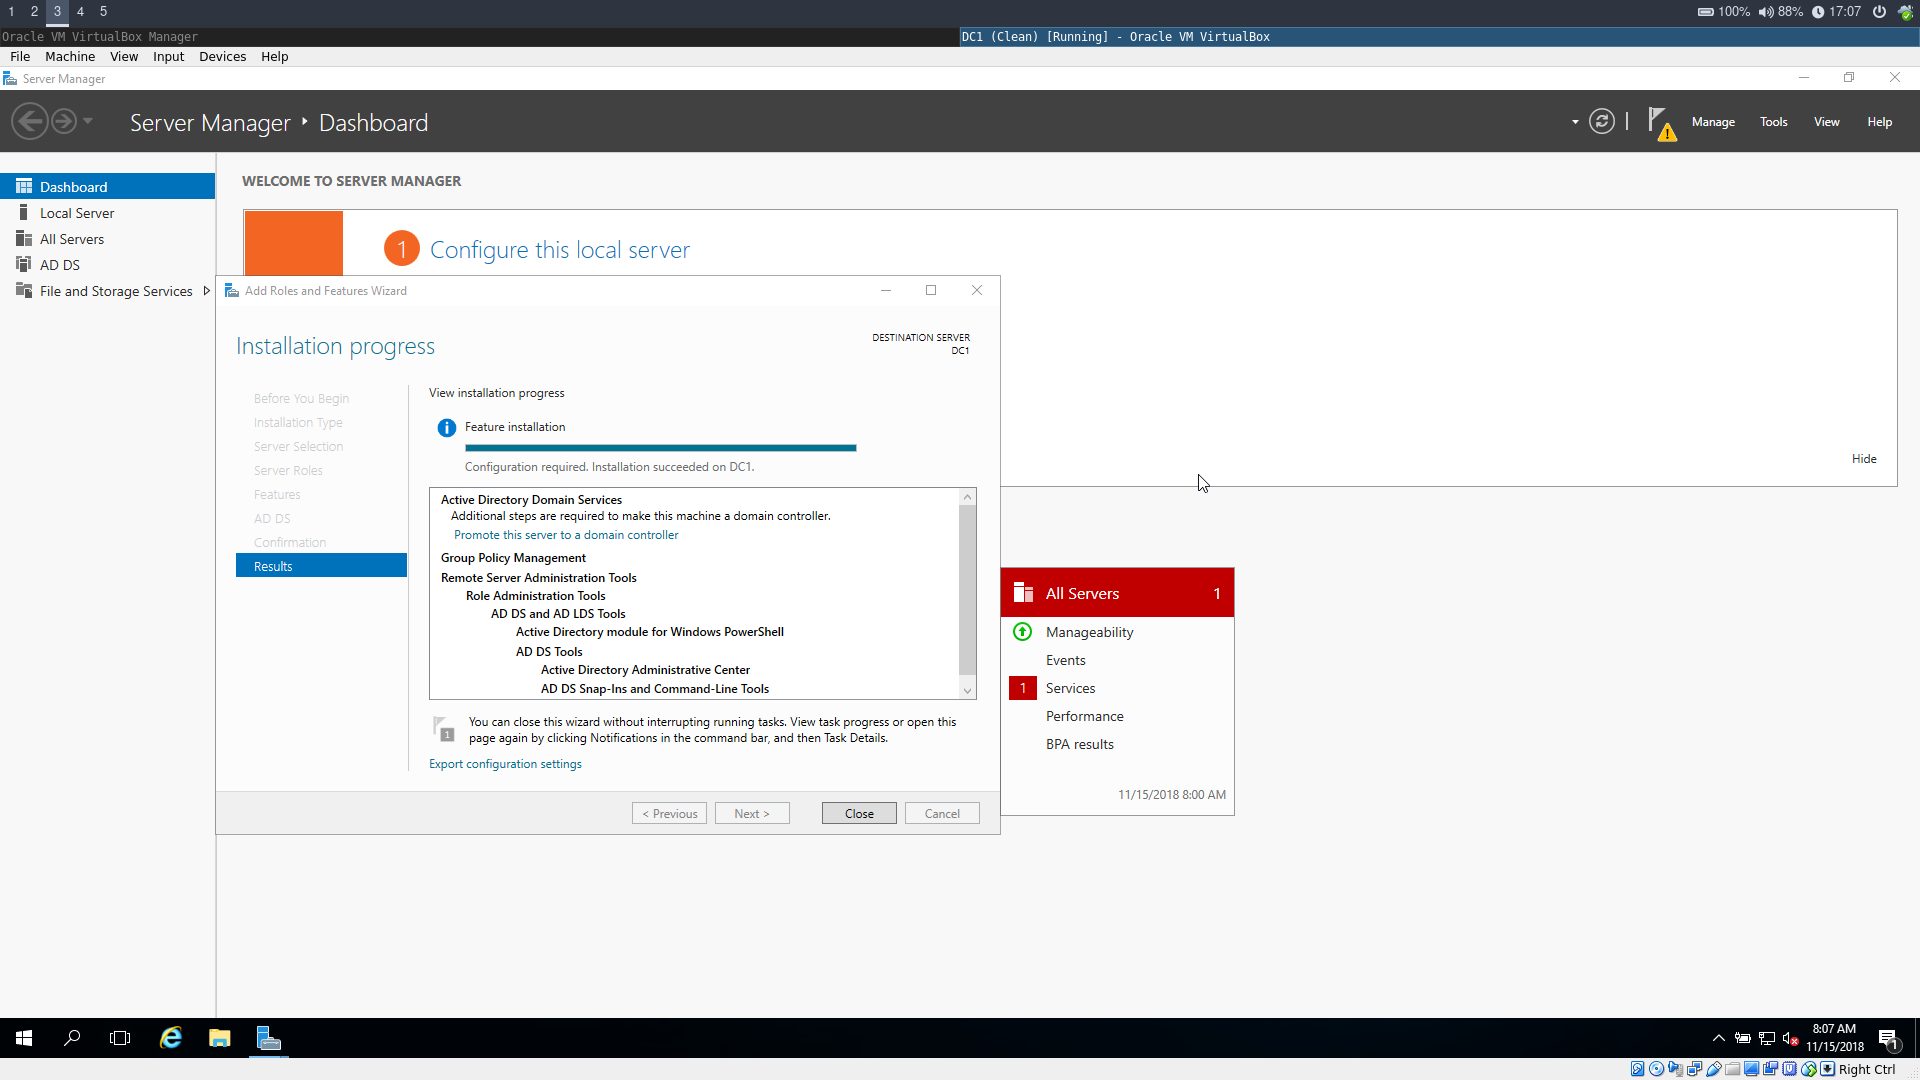
\includegraphics[width=15cm]{Pictures/DC1/ADDS/1542298075.png}
	
	Volg de installatiewizard.
\end{center}
\begin{center}
	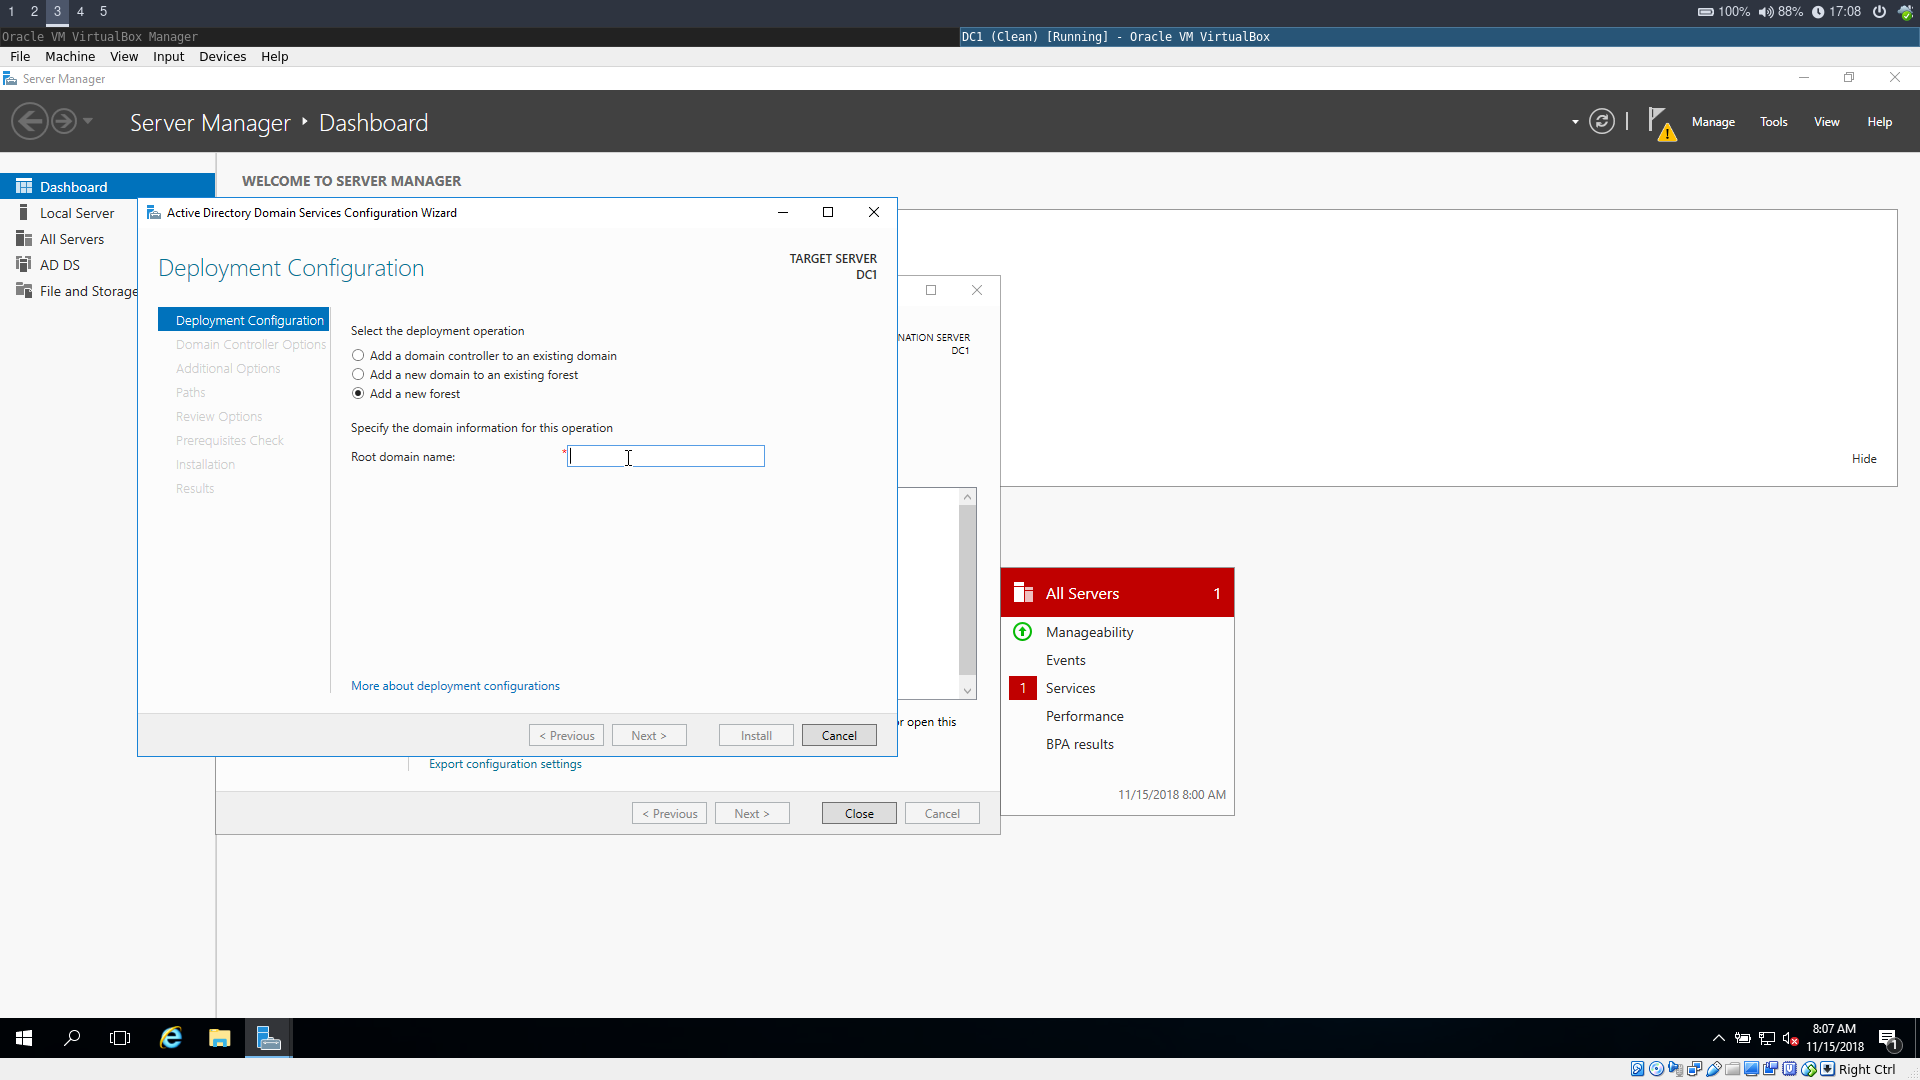
\includegraphics[width=15cm]{Pictures/DC1/ADDS/1542298094.png}
	
	Selecteer het aanmaken van een nieuw forest.
\end{center}
\begin{center}
	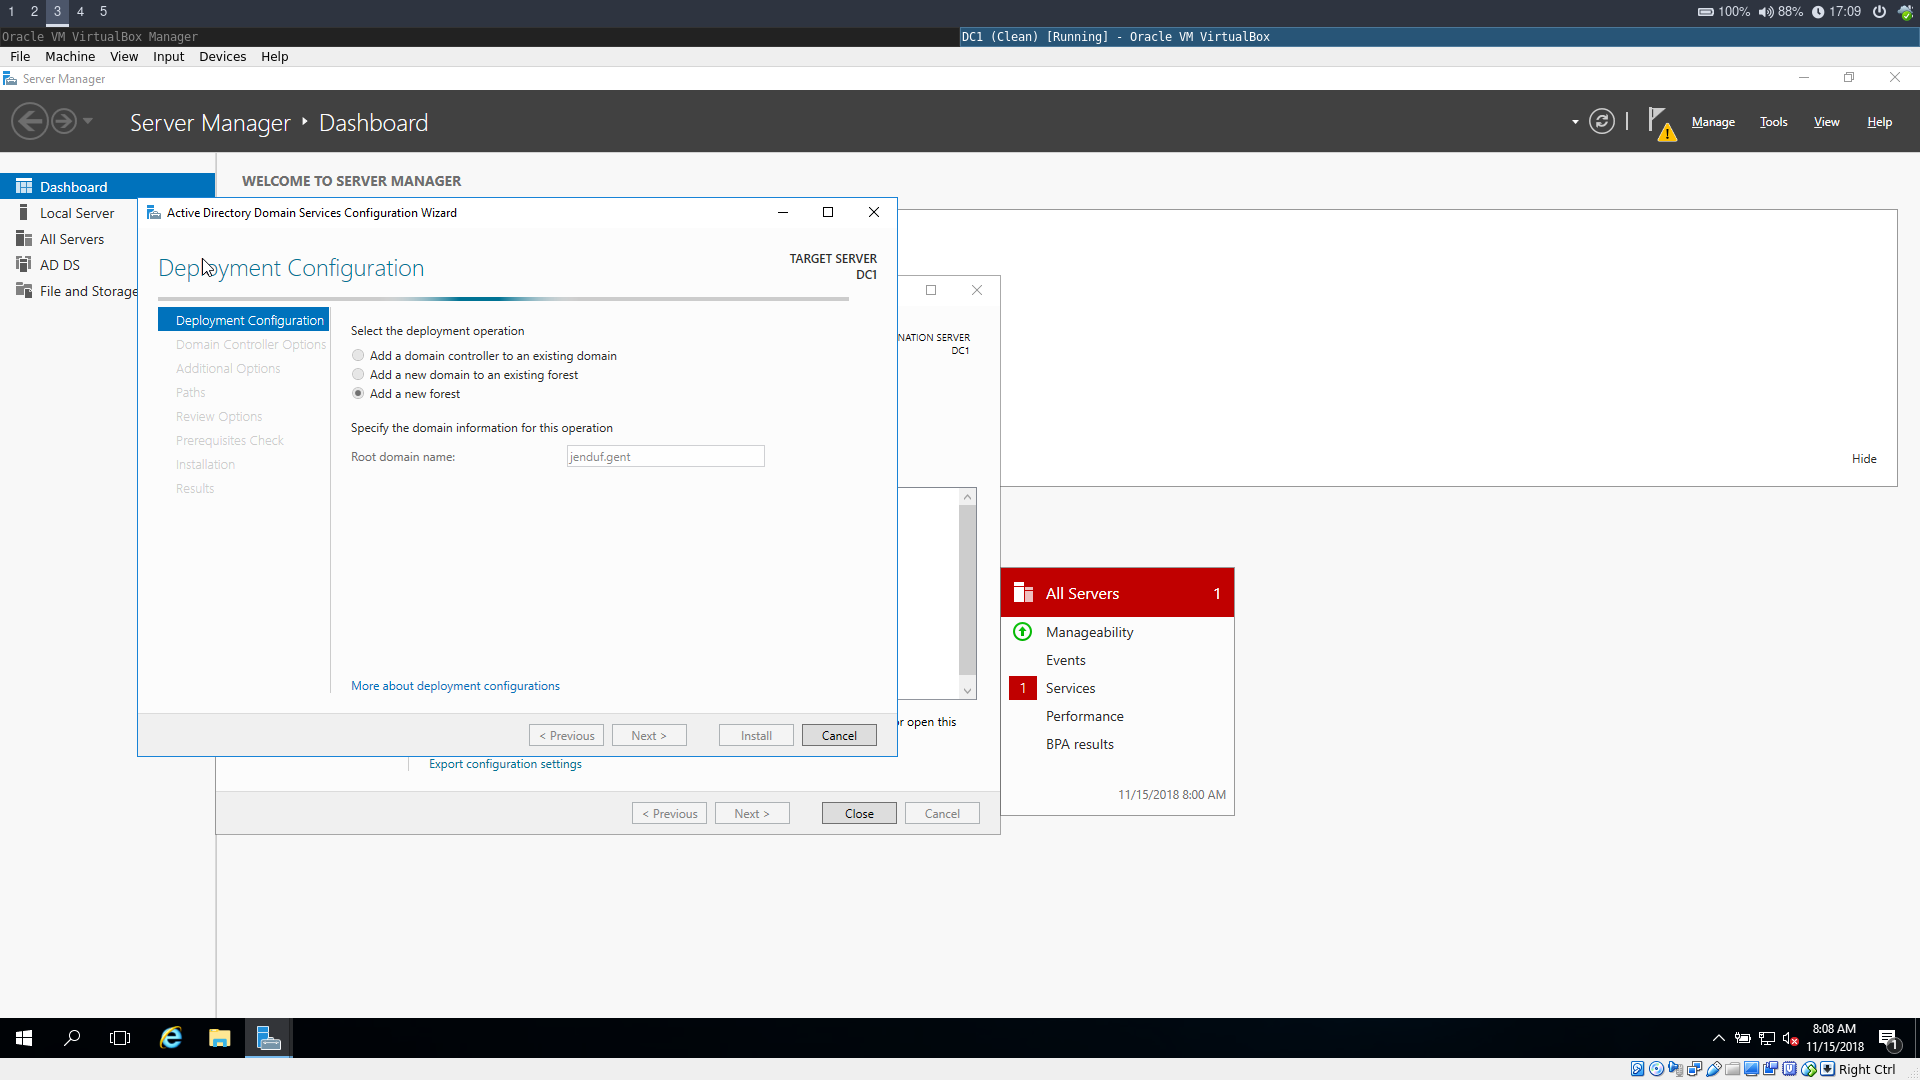
\includegraphics[width=15cm]{Pictures/DC1/ADDS/1542298140.png}
	
	Kies als domeinnaam "jenduf.gent"
\end{center}
\begin{center}
	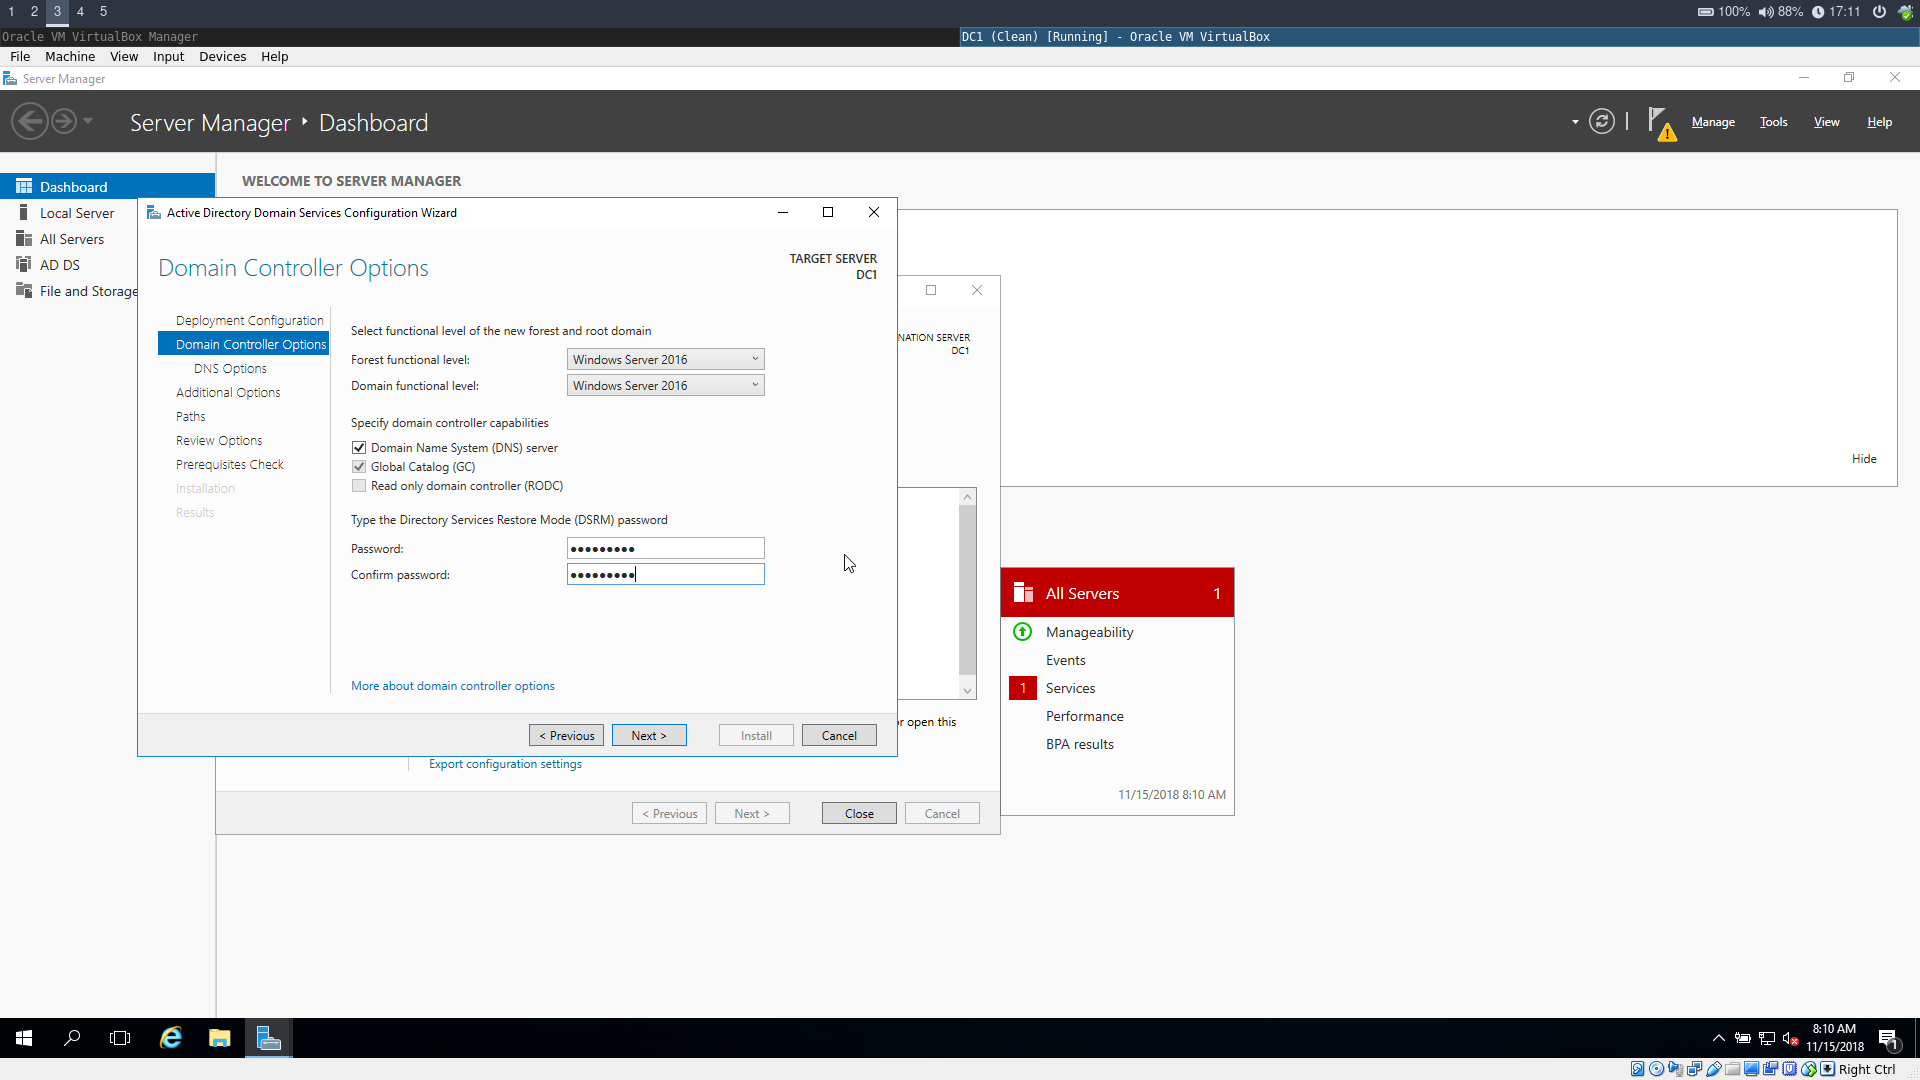
\includegraphics[width=15cm]{Pictures/DC1/ADDS/1542298296.png}
	
	Selecteer functieniveau Windows Server 2016 en kies paswoord Admin2018
\end{center}
\begin{center}
	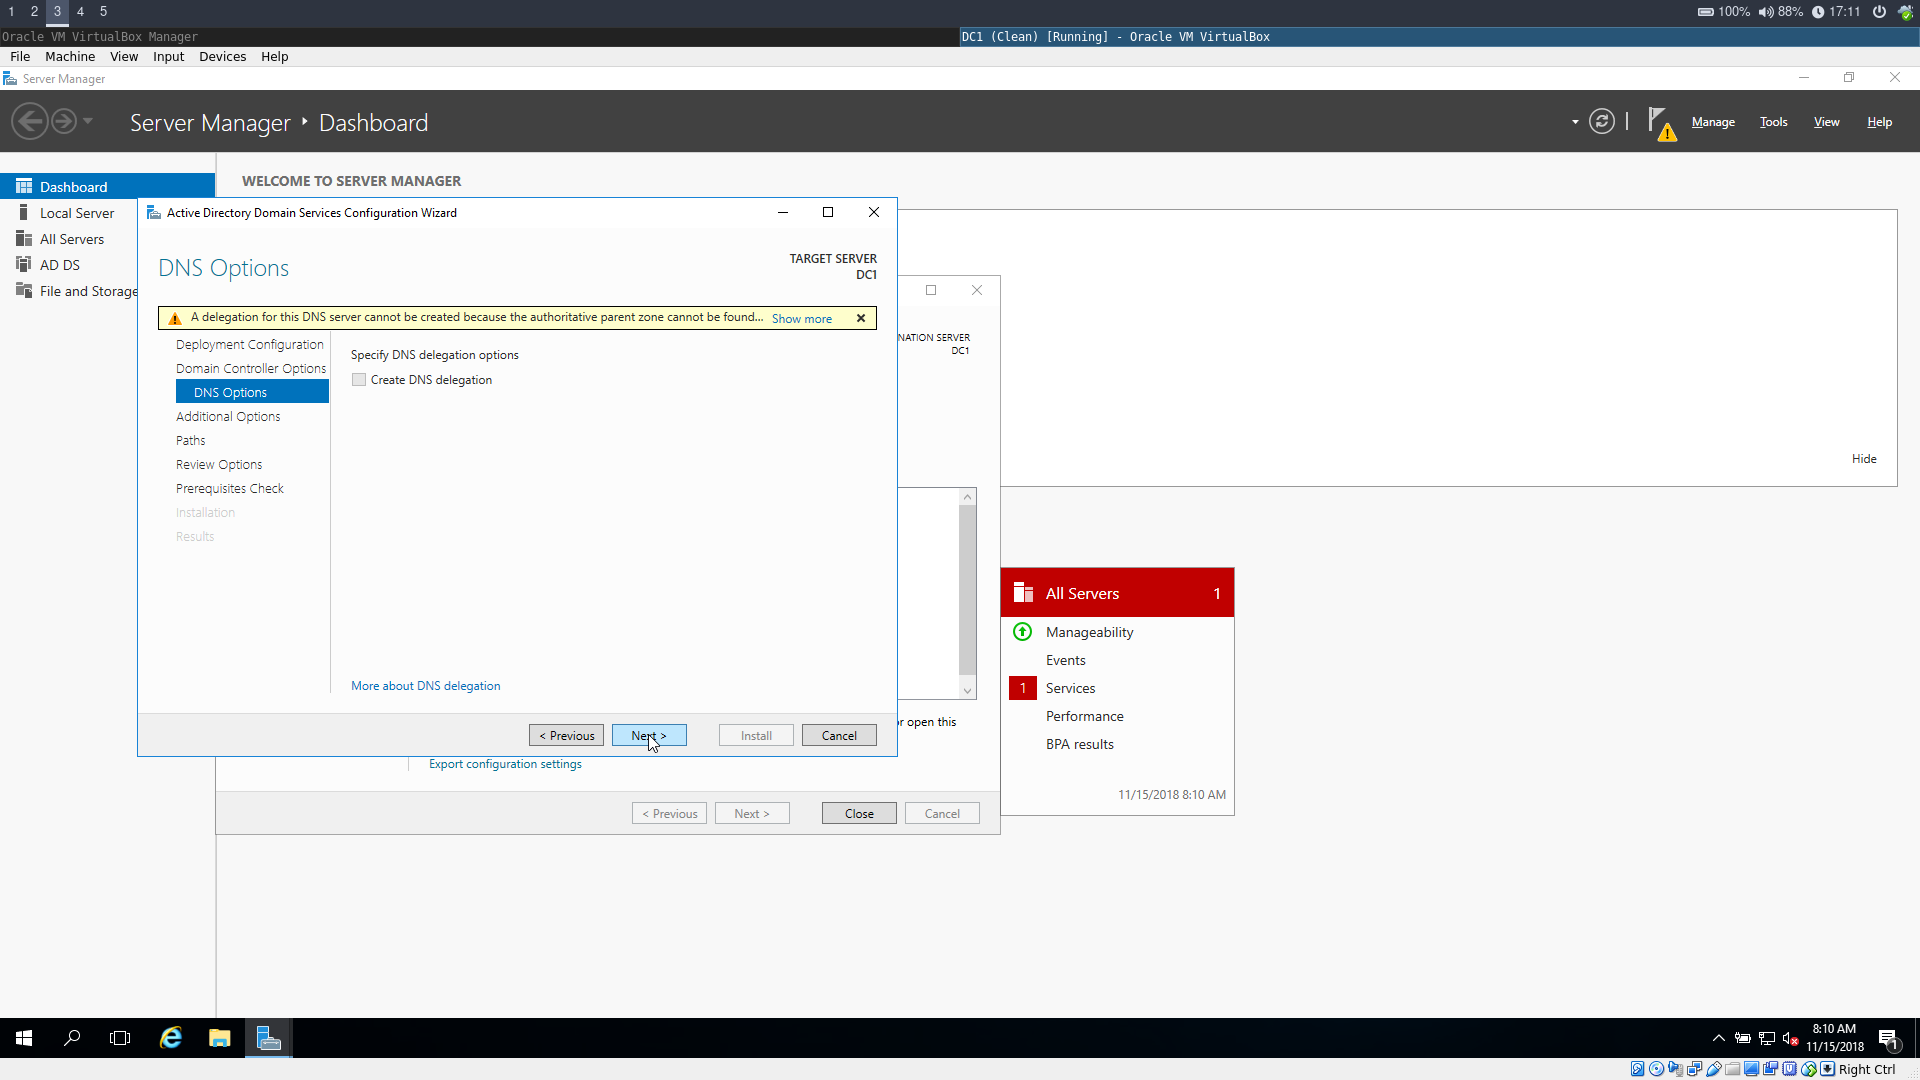
\includegraphics[width=15cm]{Pictures/DC1/ADDS/1542298300.png}
	
	Volg de configuratiewizard verder.
\end{center}
\begin{center}
	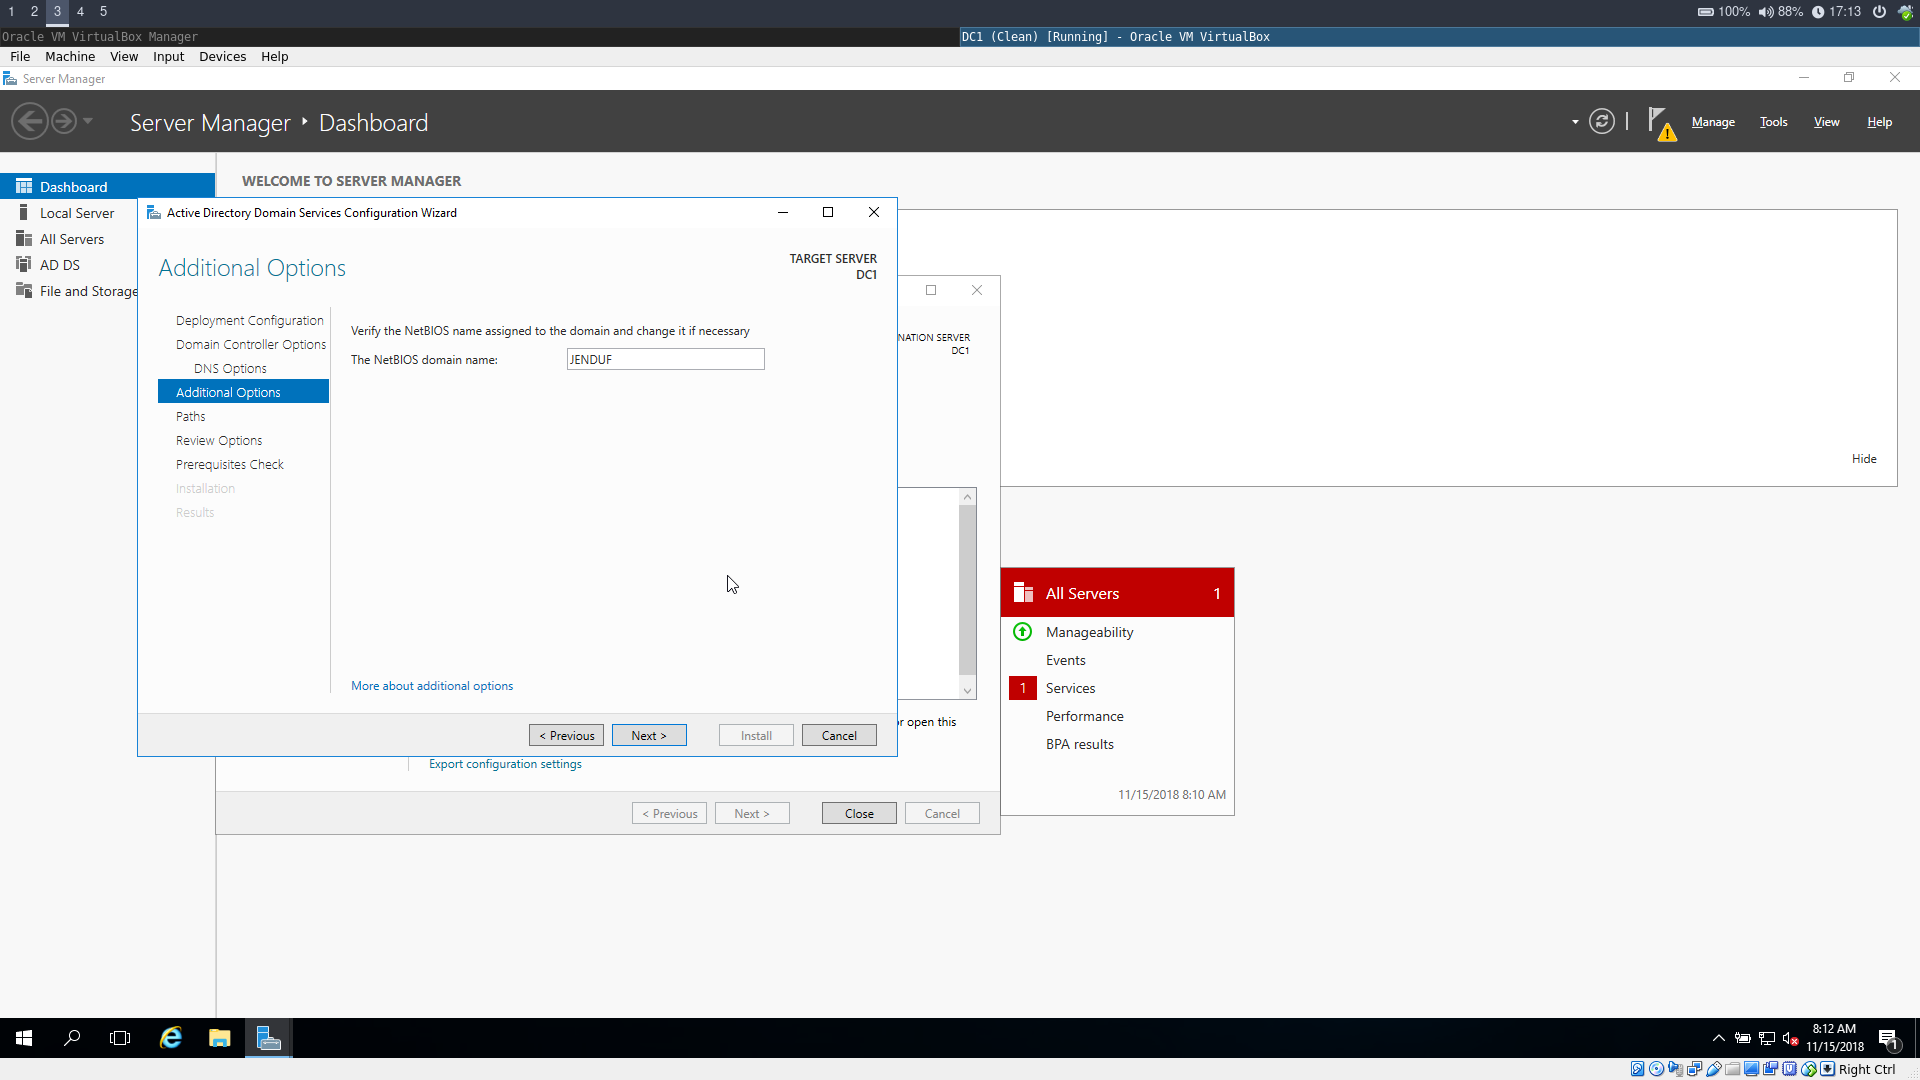
\includegraphics[width=15cm]{Pictures/DC1/ADDS/1542298389.png}
	
	Stel "JENDUF" in als NetBIOS domeinnaam.
\end{center}
\begin{center}
	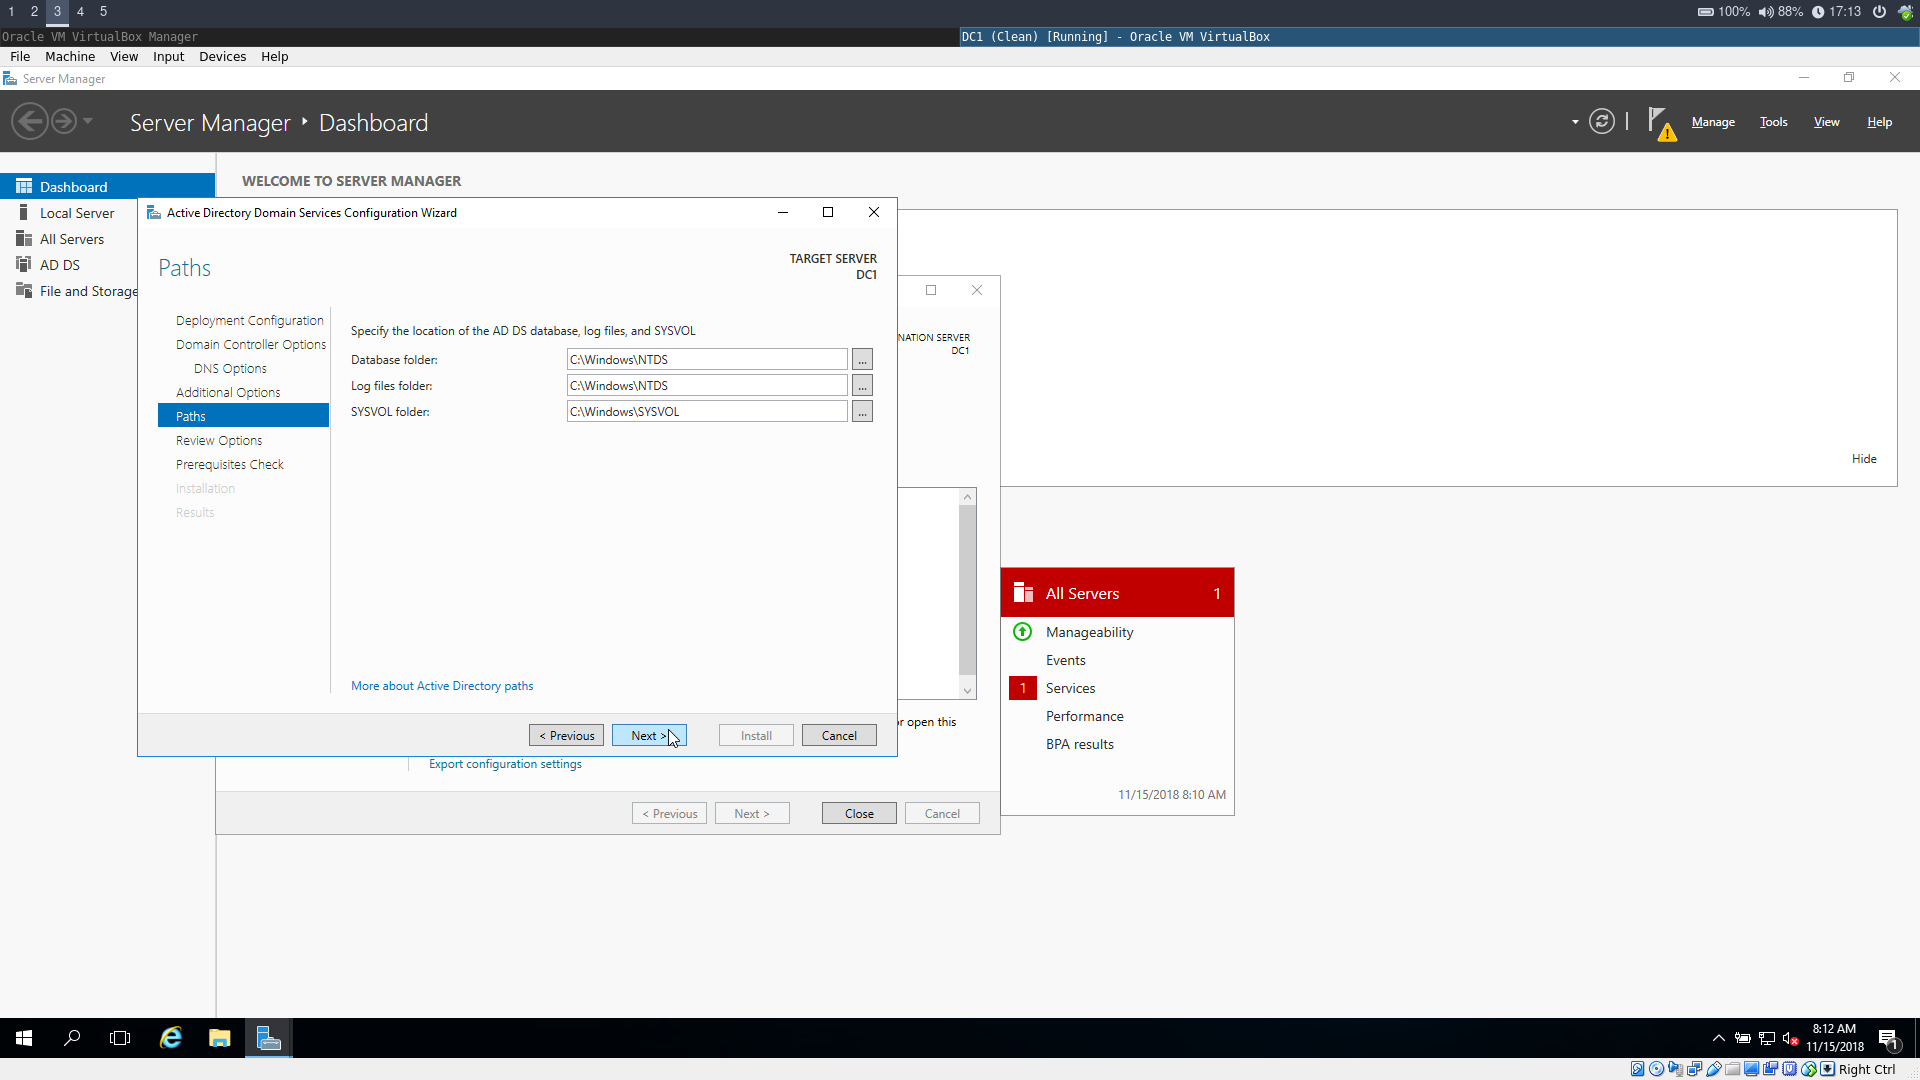
\includegraphics[width=15cm]{Pictures/DC1/ADDS/1542298414.png}
\end{center}
\begin{center}
	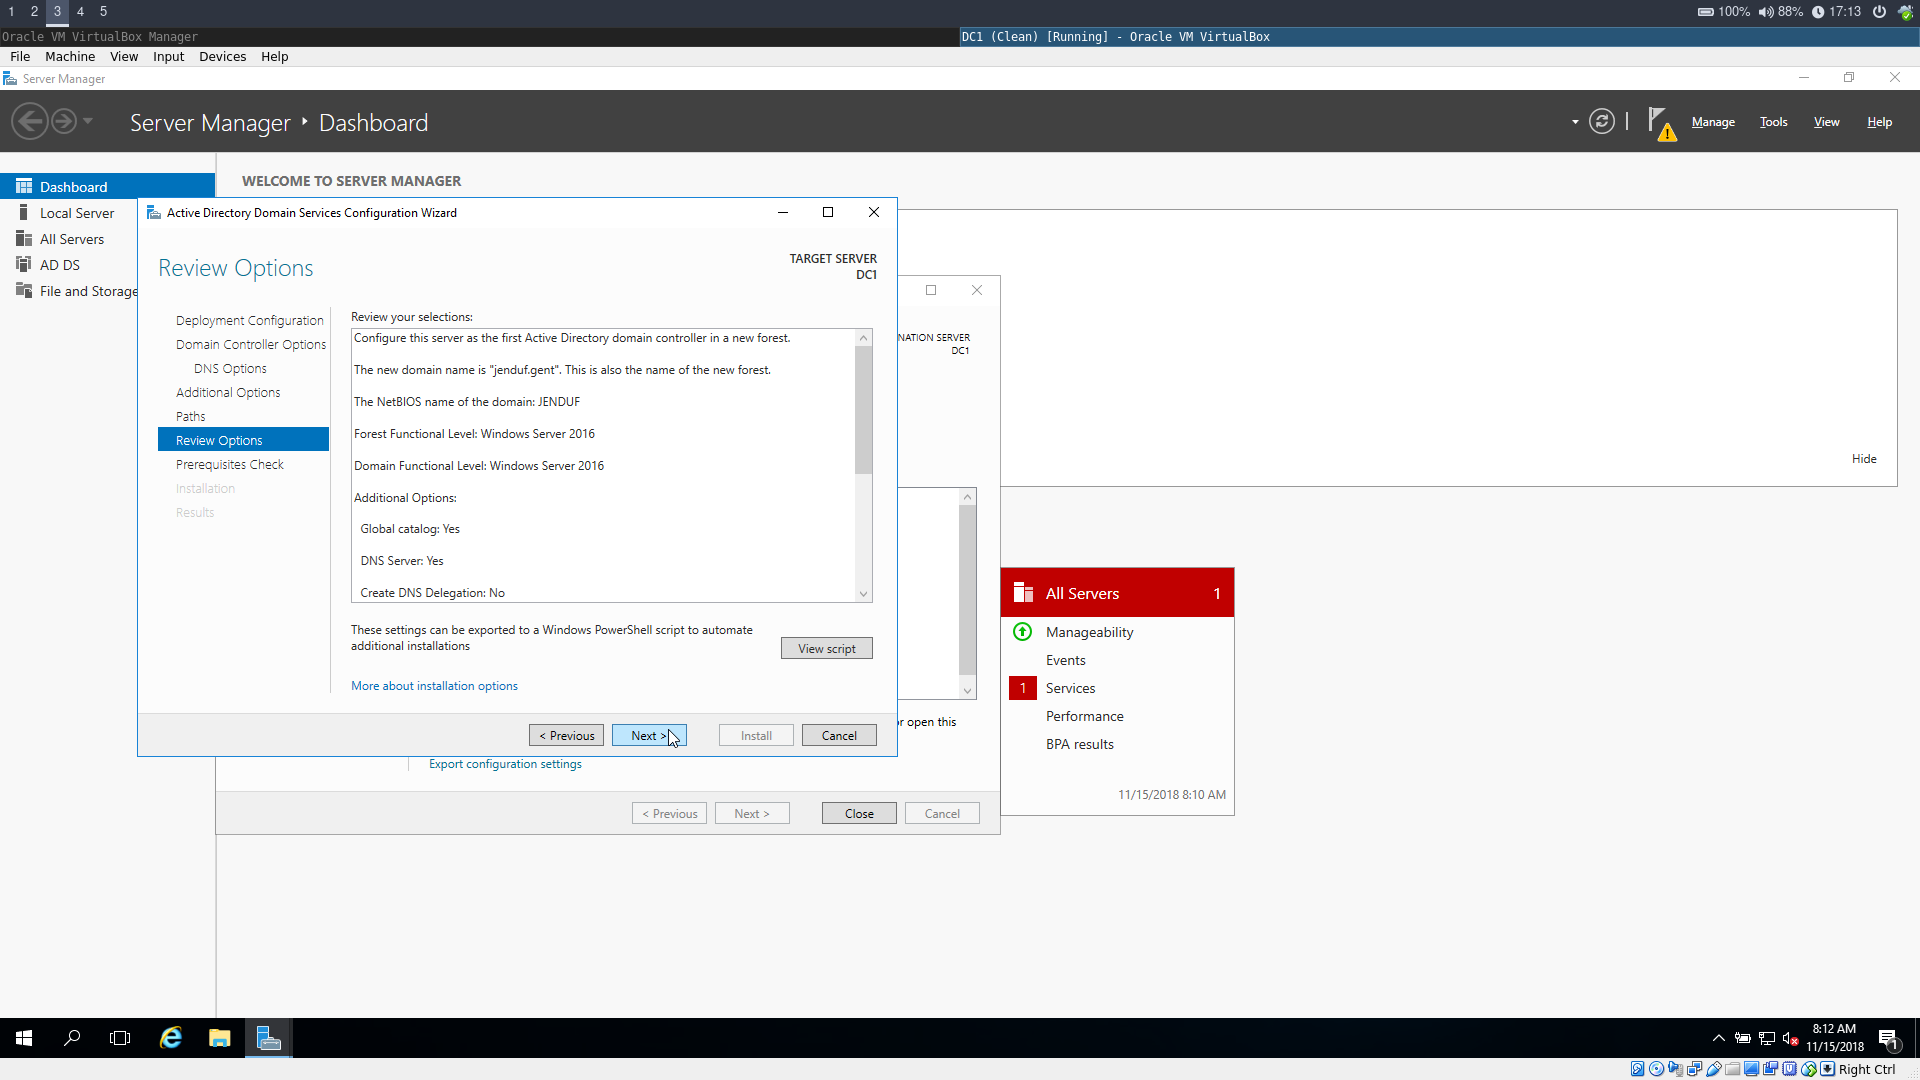
\includegraphics[width=15cm]{Pictures/DC1/ADDS/1542298418.png}
\end{center}
\begin{center}
	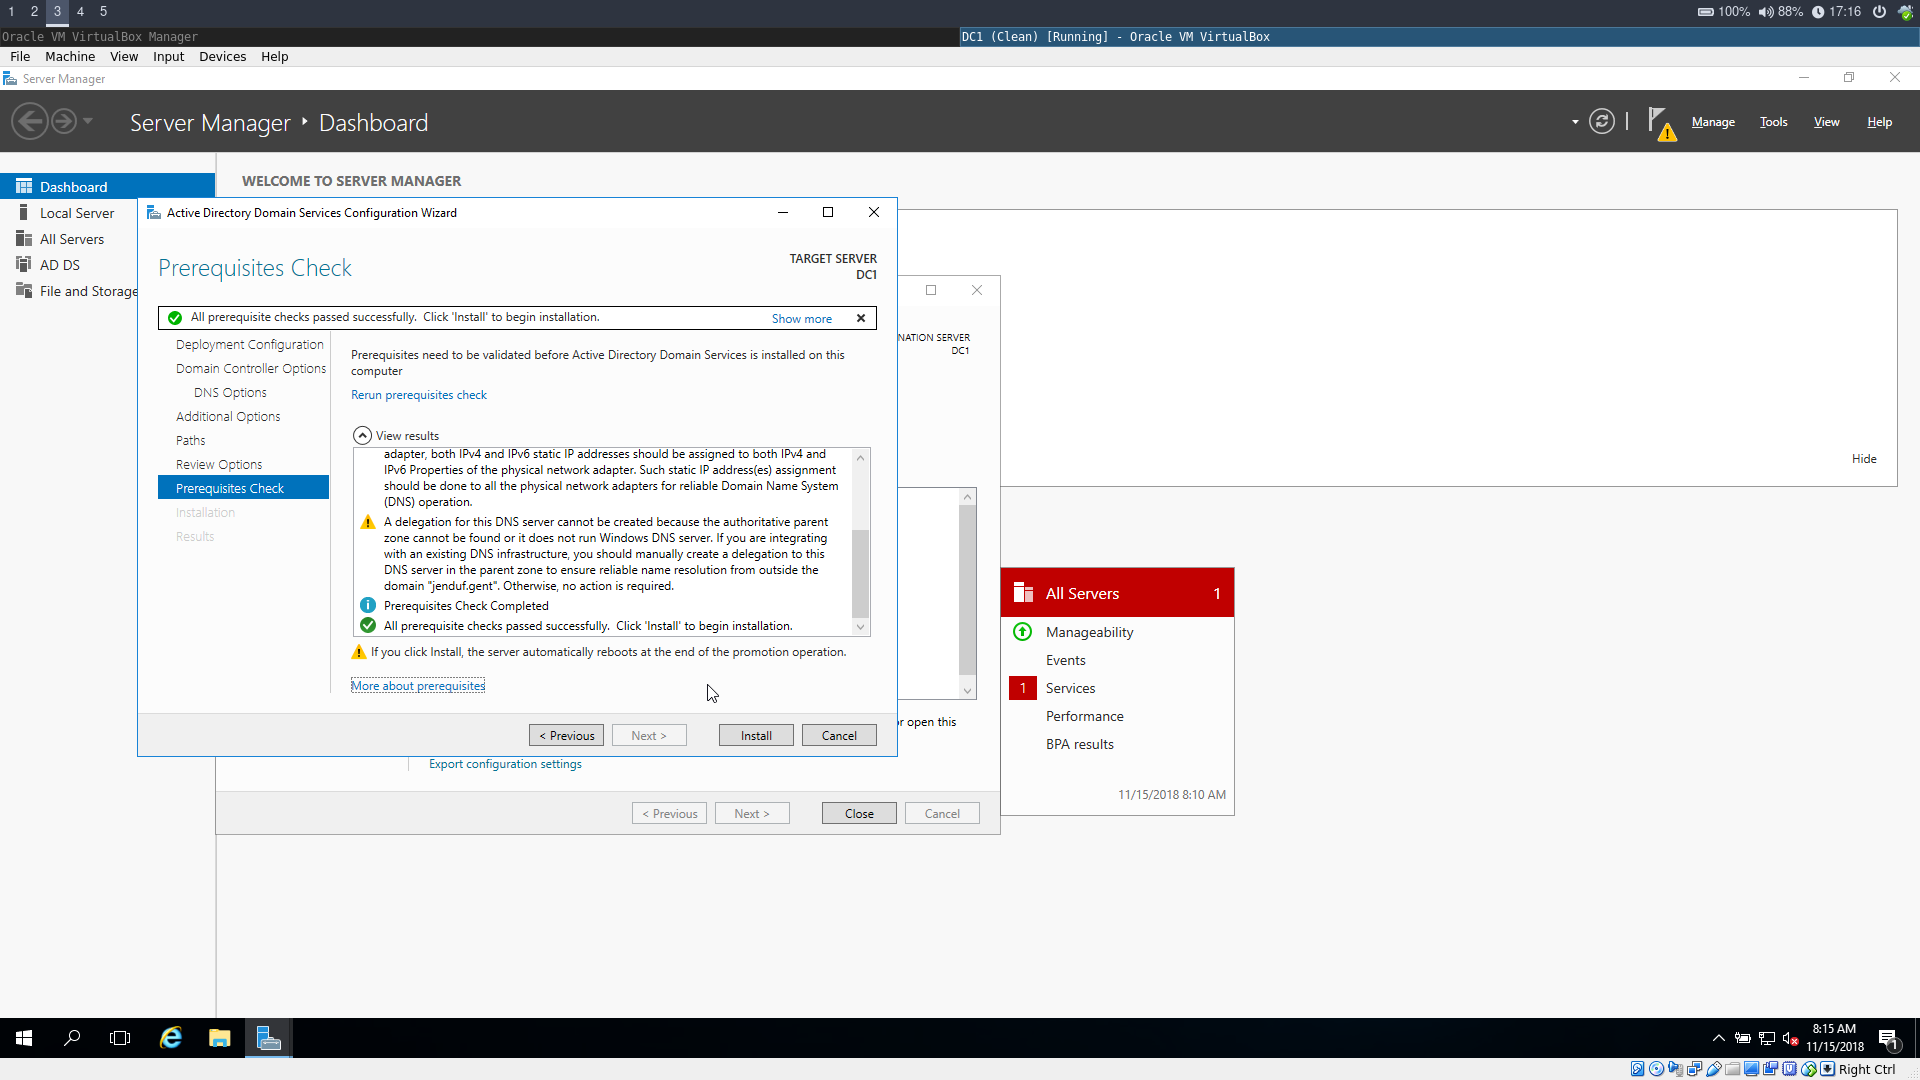
\includegraphics[width=15cm]{Pictures/DC1/ADDS/1542298569.png}
\end{center}
\begin{center}
	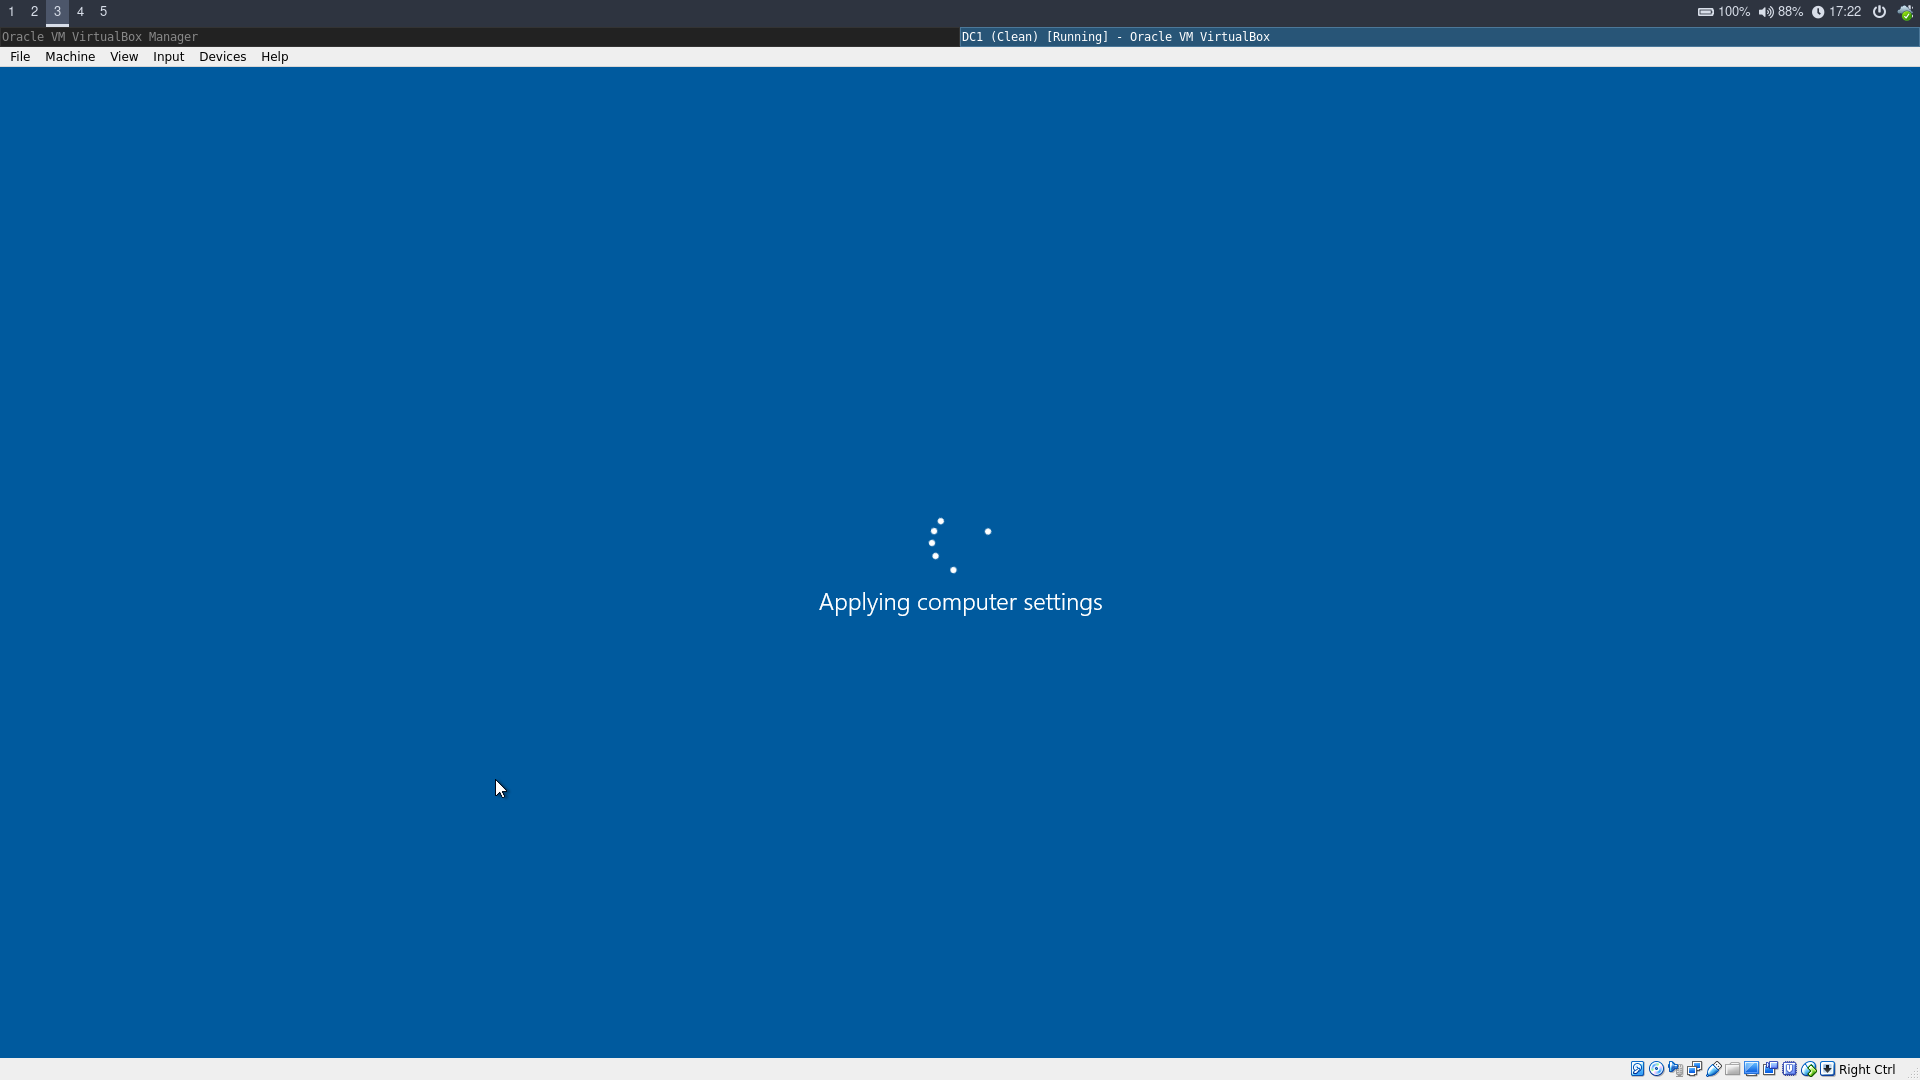
\includegraphics[width=15cm]{Pictures/DC1/ADDS/1542298968.png}
	
	Na het heropstarten is de ADDS geinstalleerd en geconfigureerd.
\end{center}
\begin{center}
	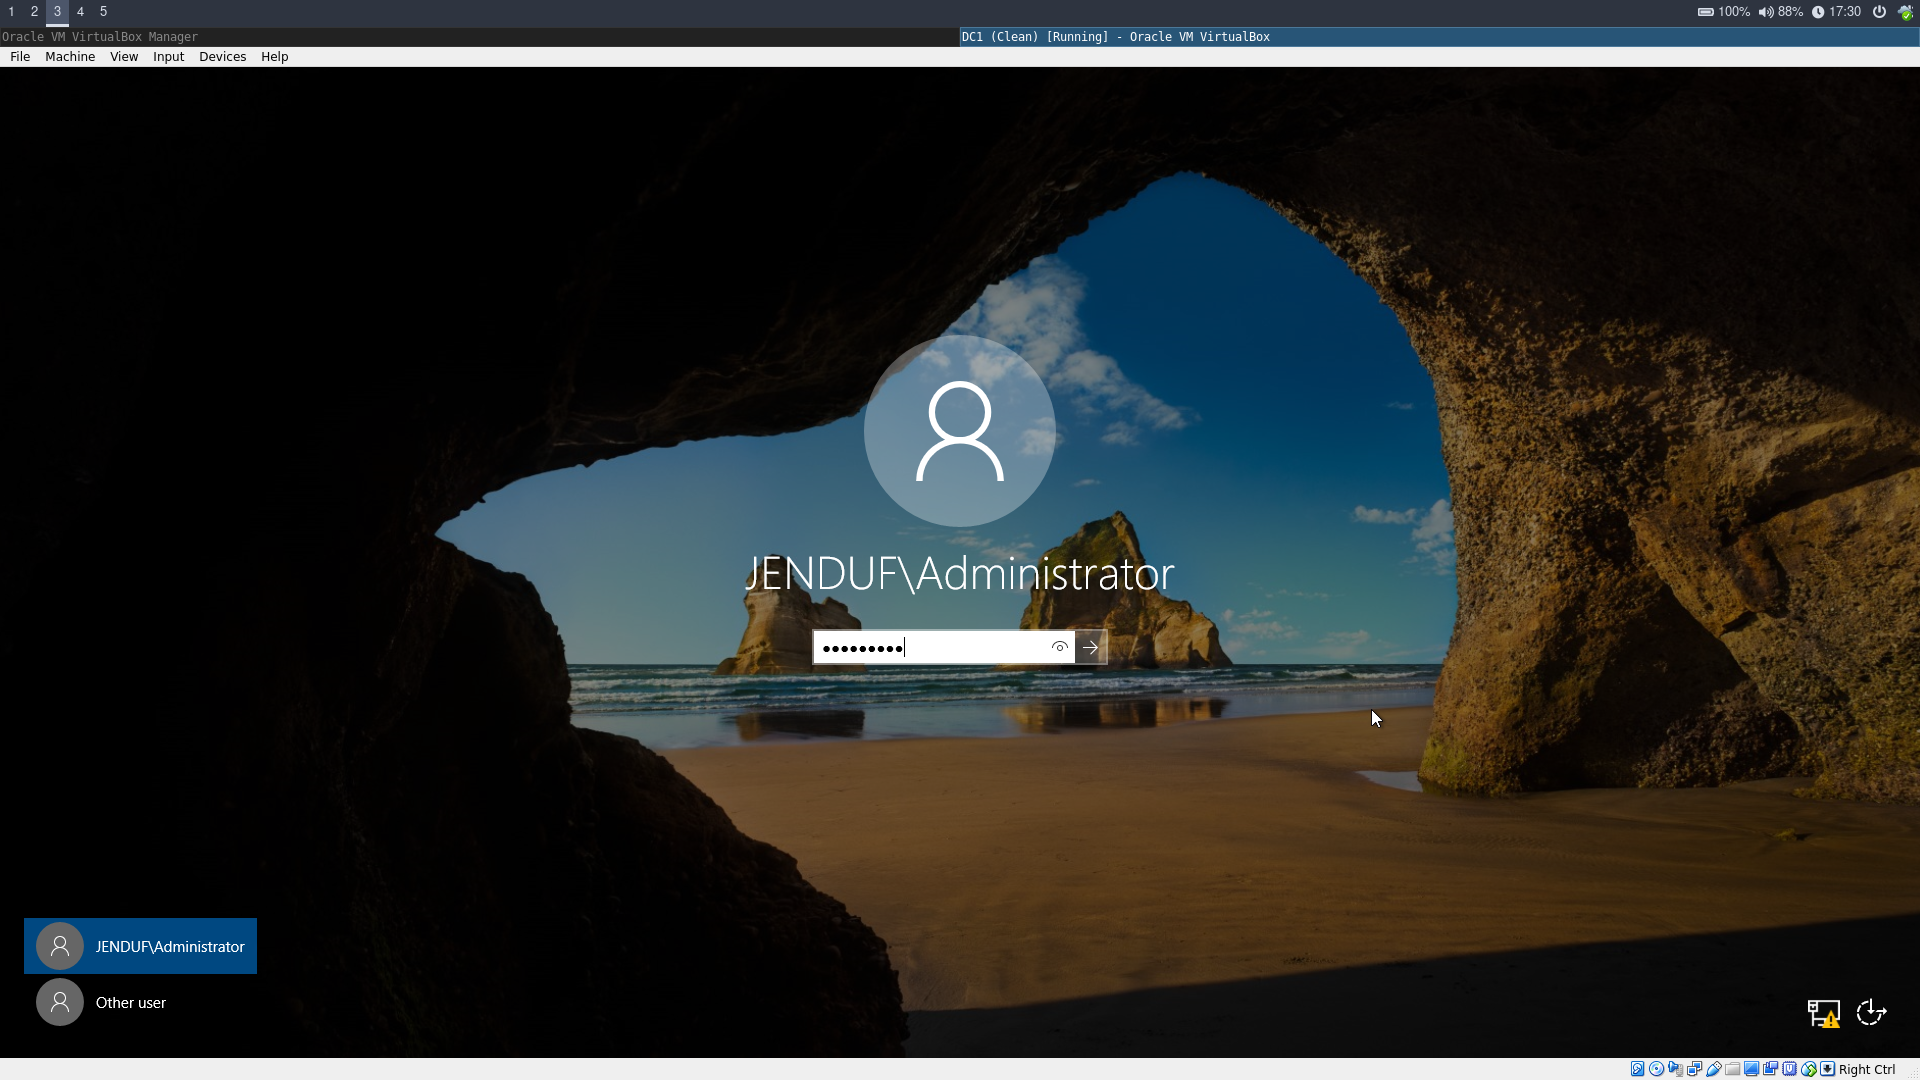
\includegraphics[width=15cm]{Pictures/DC1/ADDS/1542299418.png}
	
	Meld aan met het paswoord Admin2018.
\end{center}
\begin{center}
	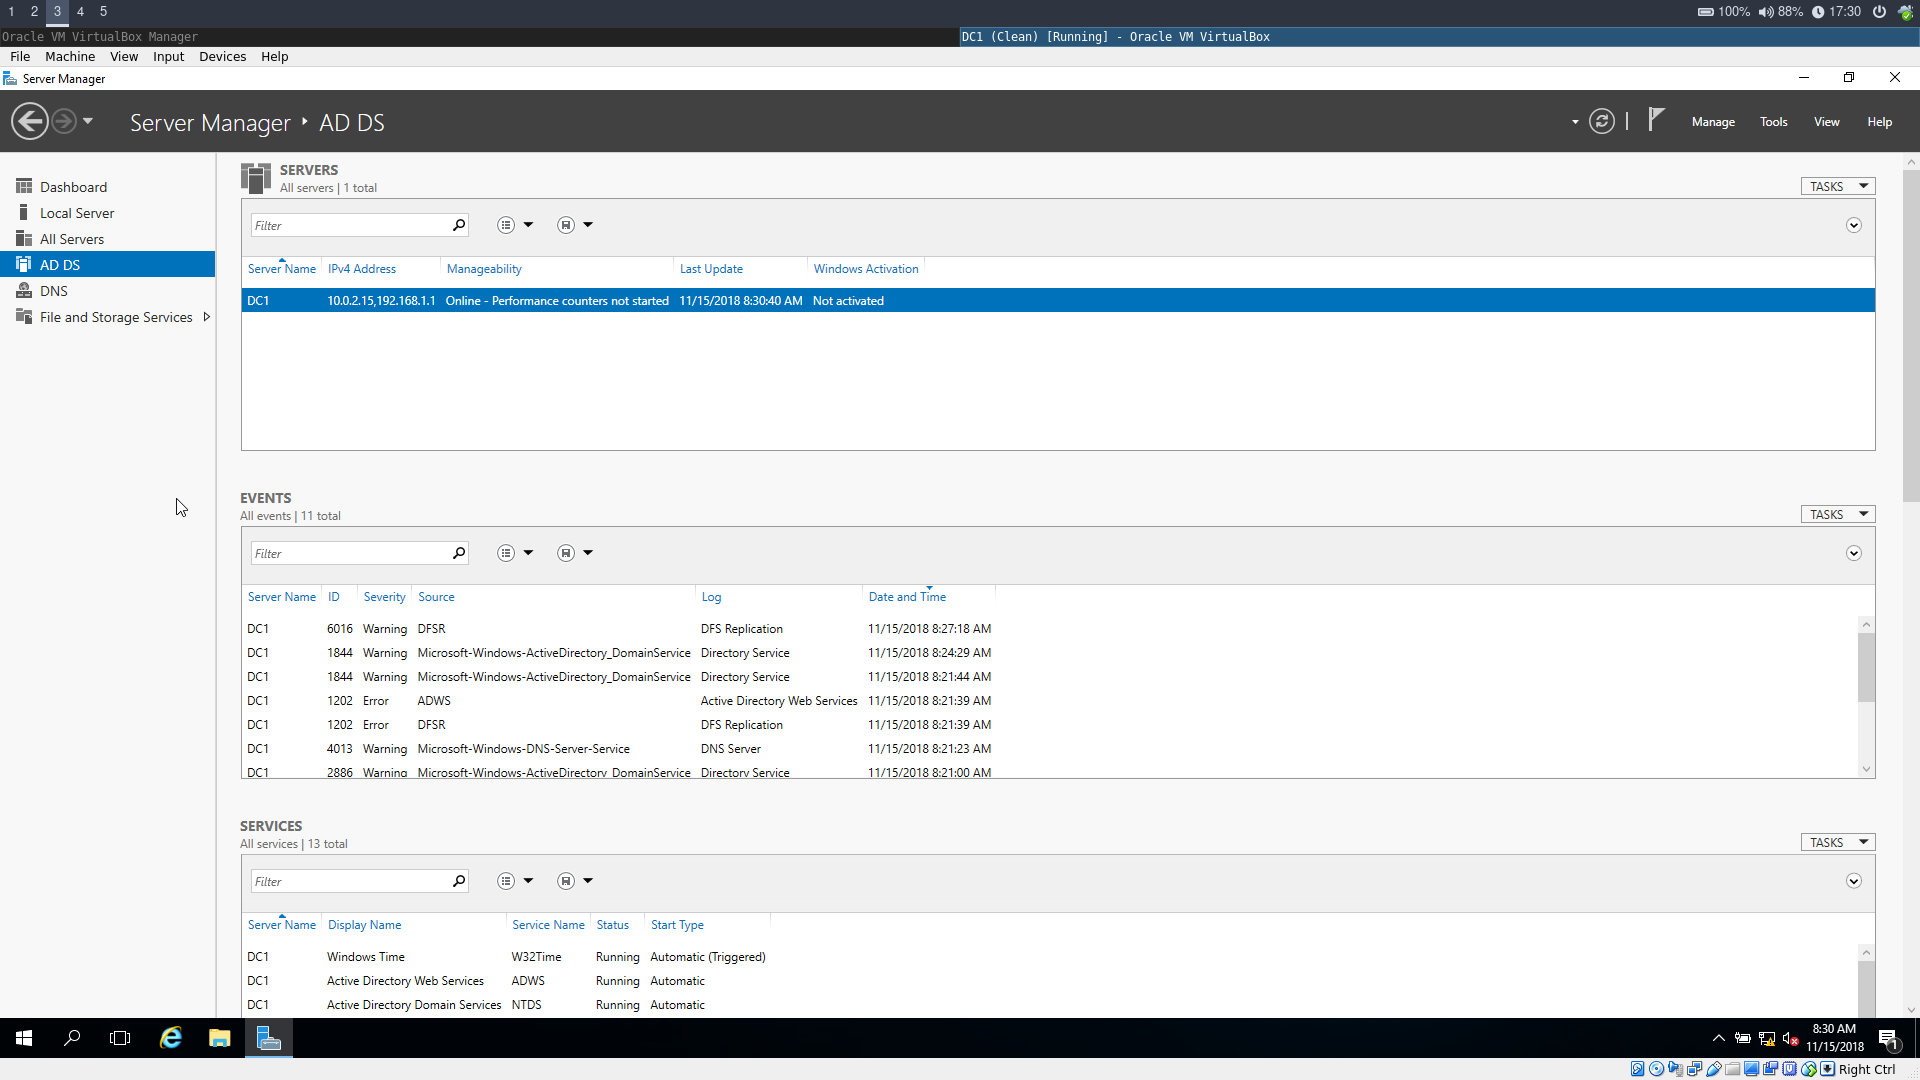
\includegraphics[width=15cm]{Pictures/DC1/ADDS/1542299460.png}
	
	De ADDS is werkend te zien.
\end{center}
\section{Configuratie DHCP}
\begin{center}
	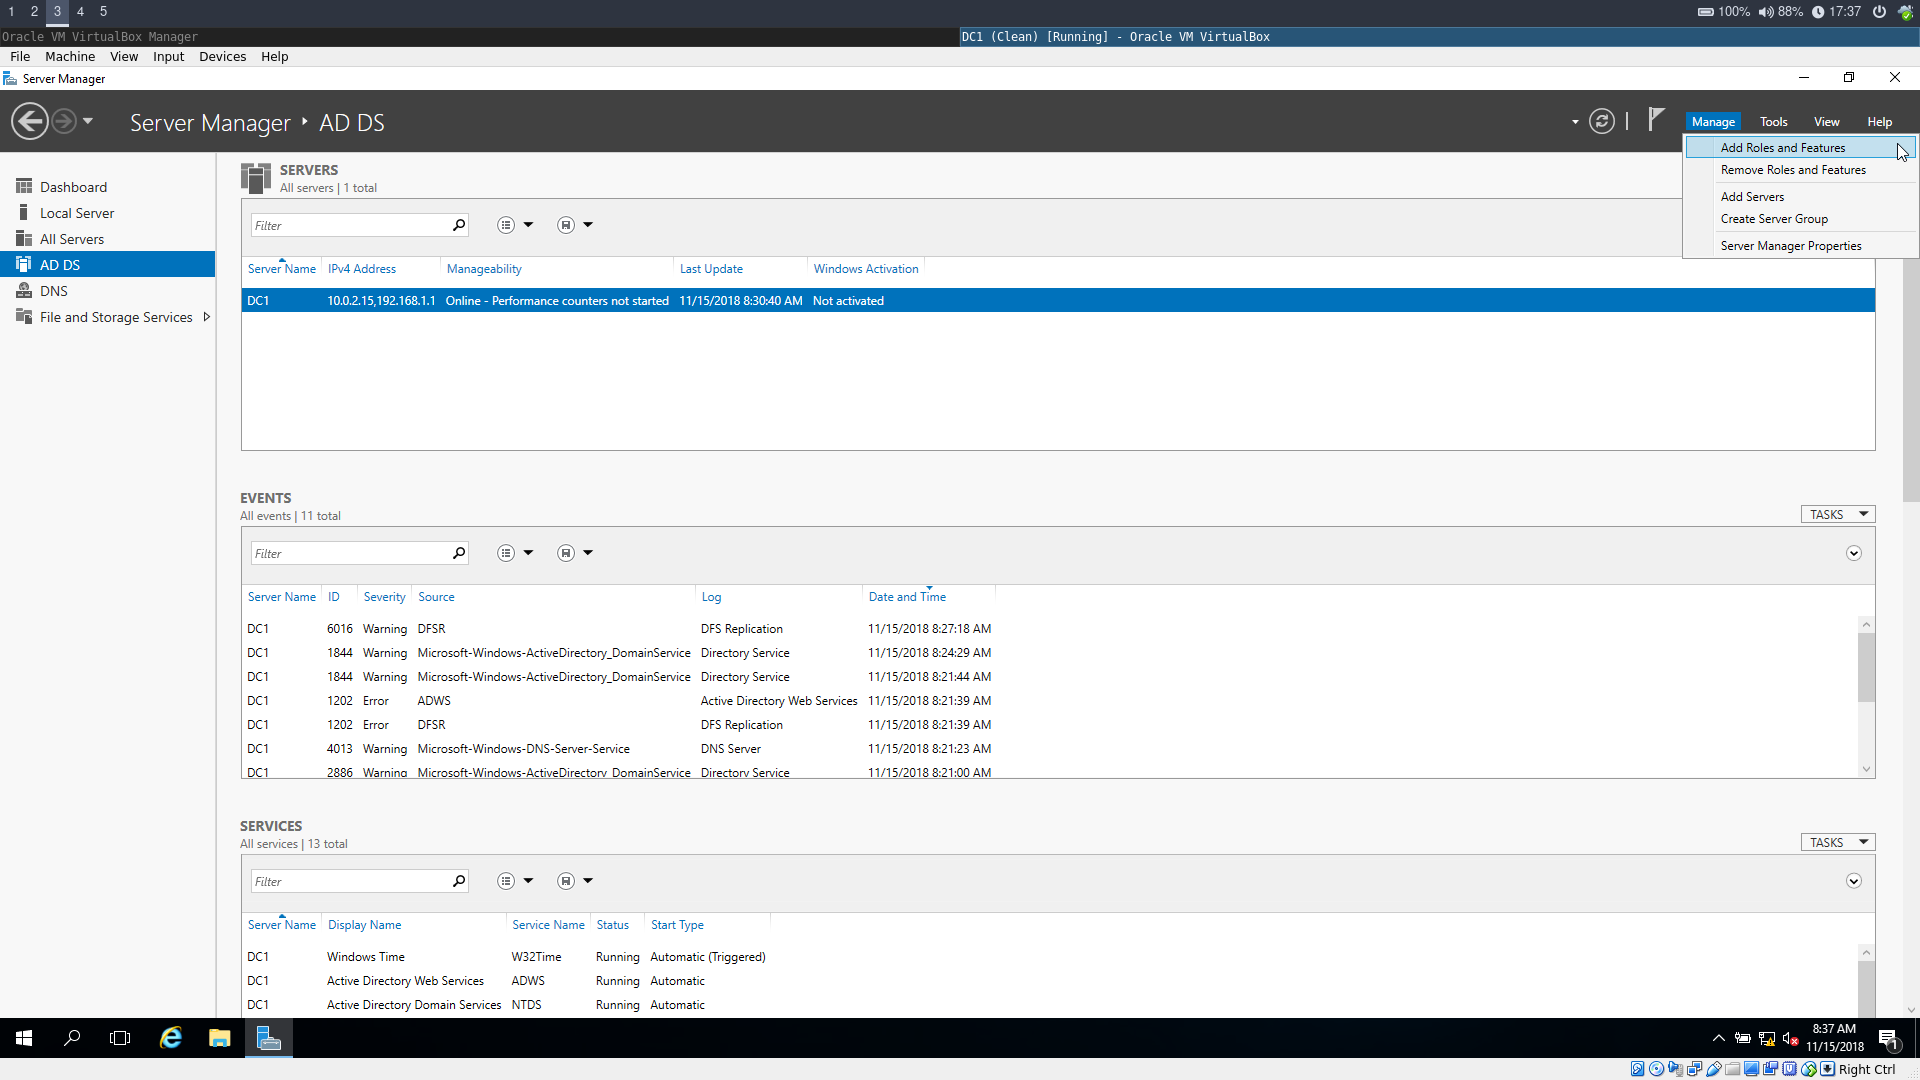
\includegraphics[width=15cm]{Pictures/DC1/DHCP/1542299853.png}
	
	Voeg een nieuwe rol toe.
\end{center}
\begin{center}
	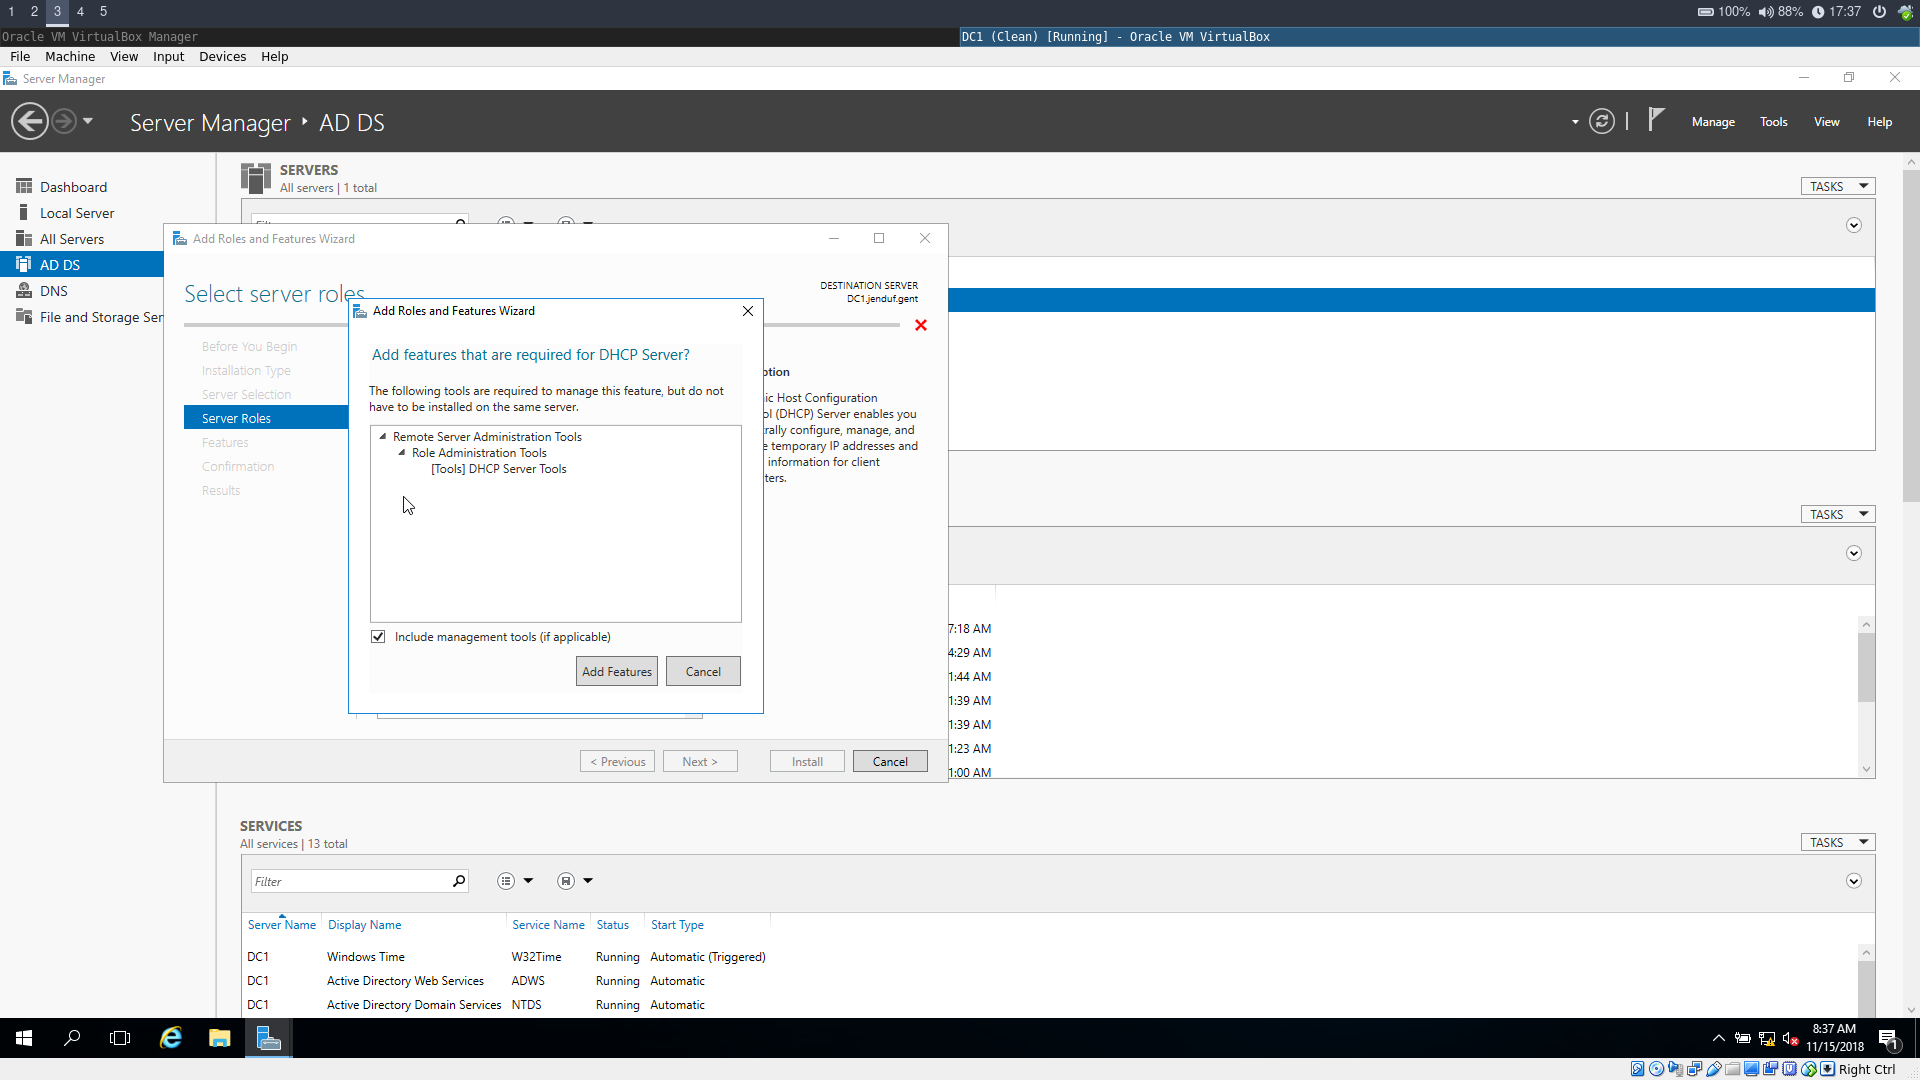
\includegraphics[width=15cm]{Pictures/DC1/DHCP/1542299861.png}
	
	Voeg de DHCP Server toe
\end{center}
\begin{center}
	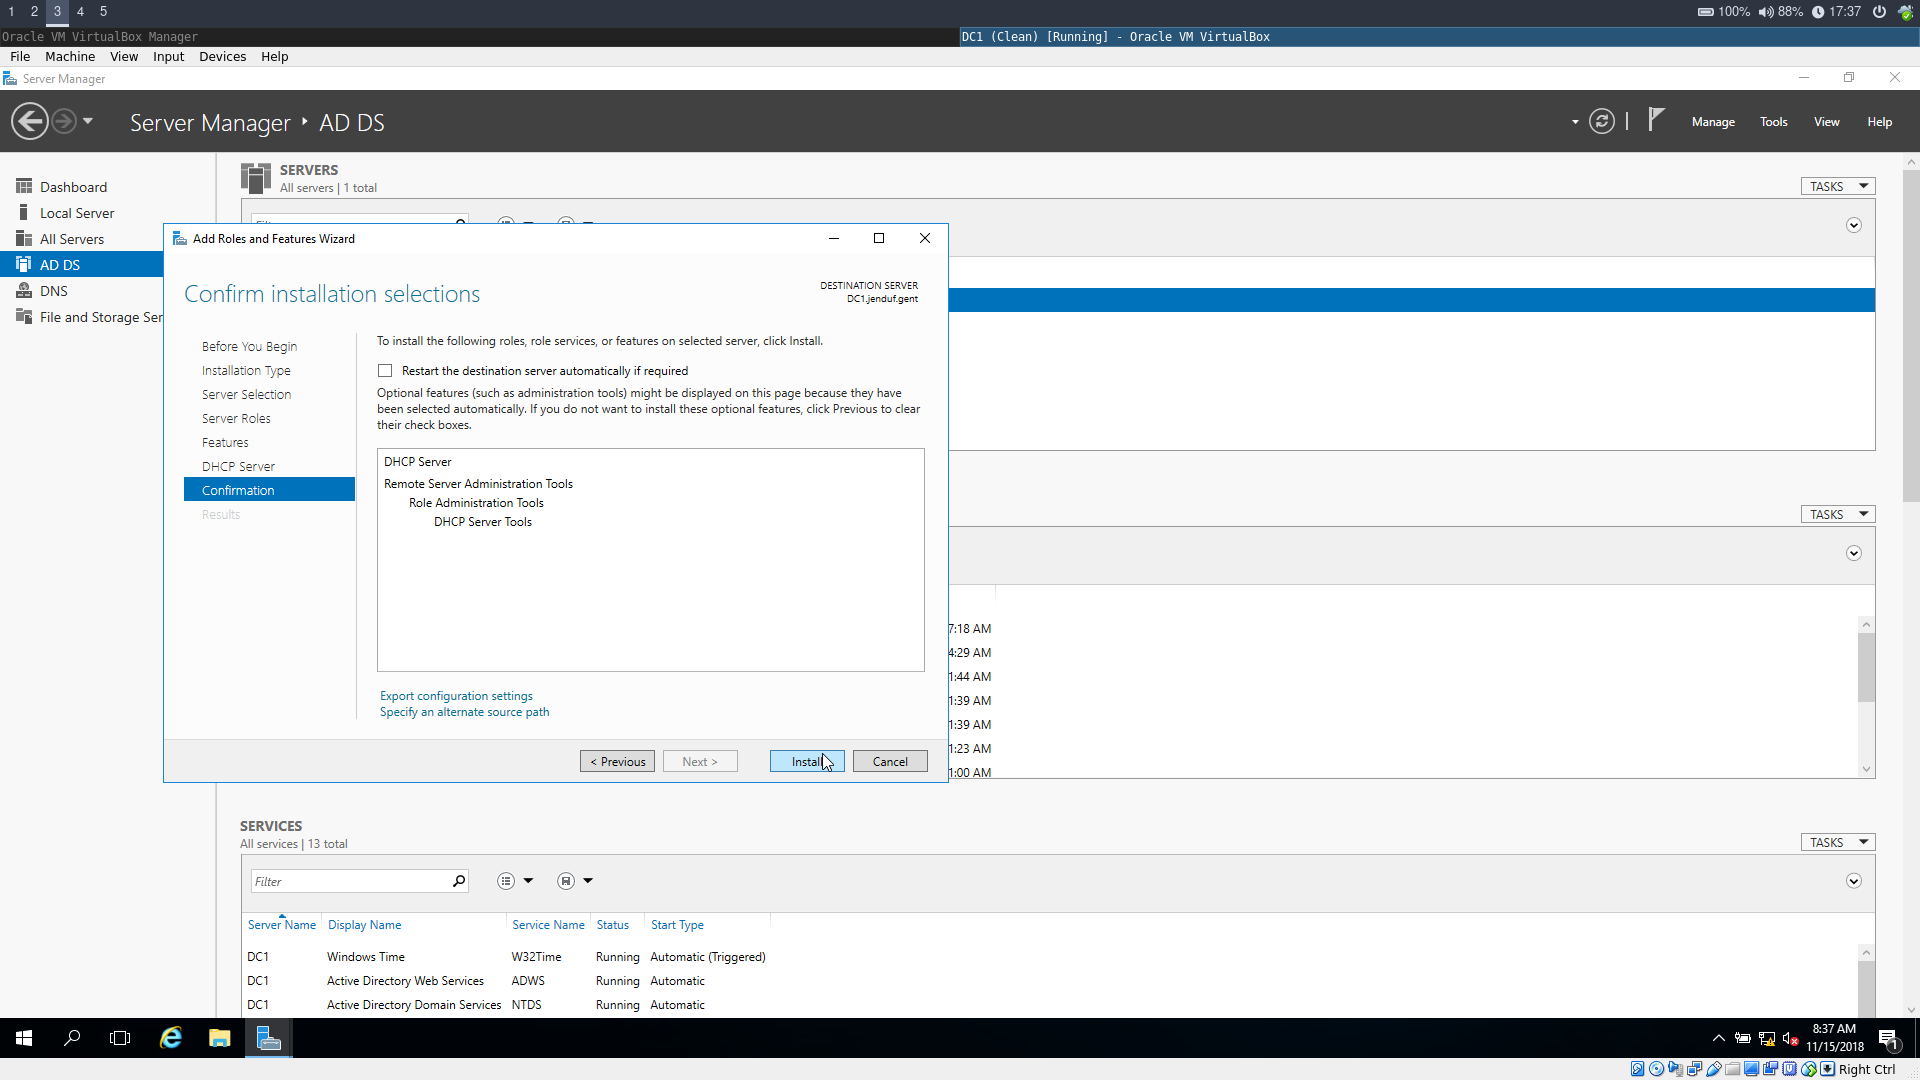
\includegraphics[width=15cm]{Pictures/DC1/DHCP/1542299870.png}
	
	Volg de installatiewizard.
\end{center}
\begin{center}
	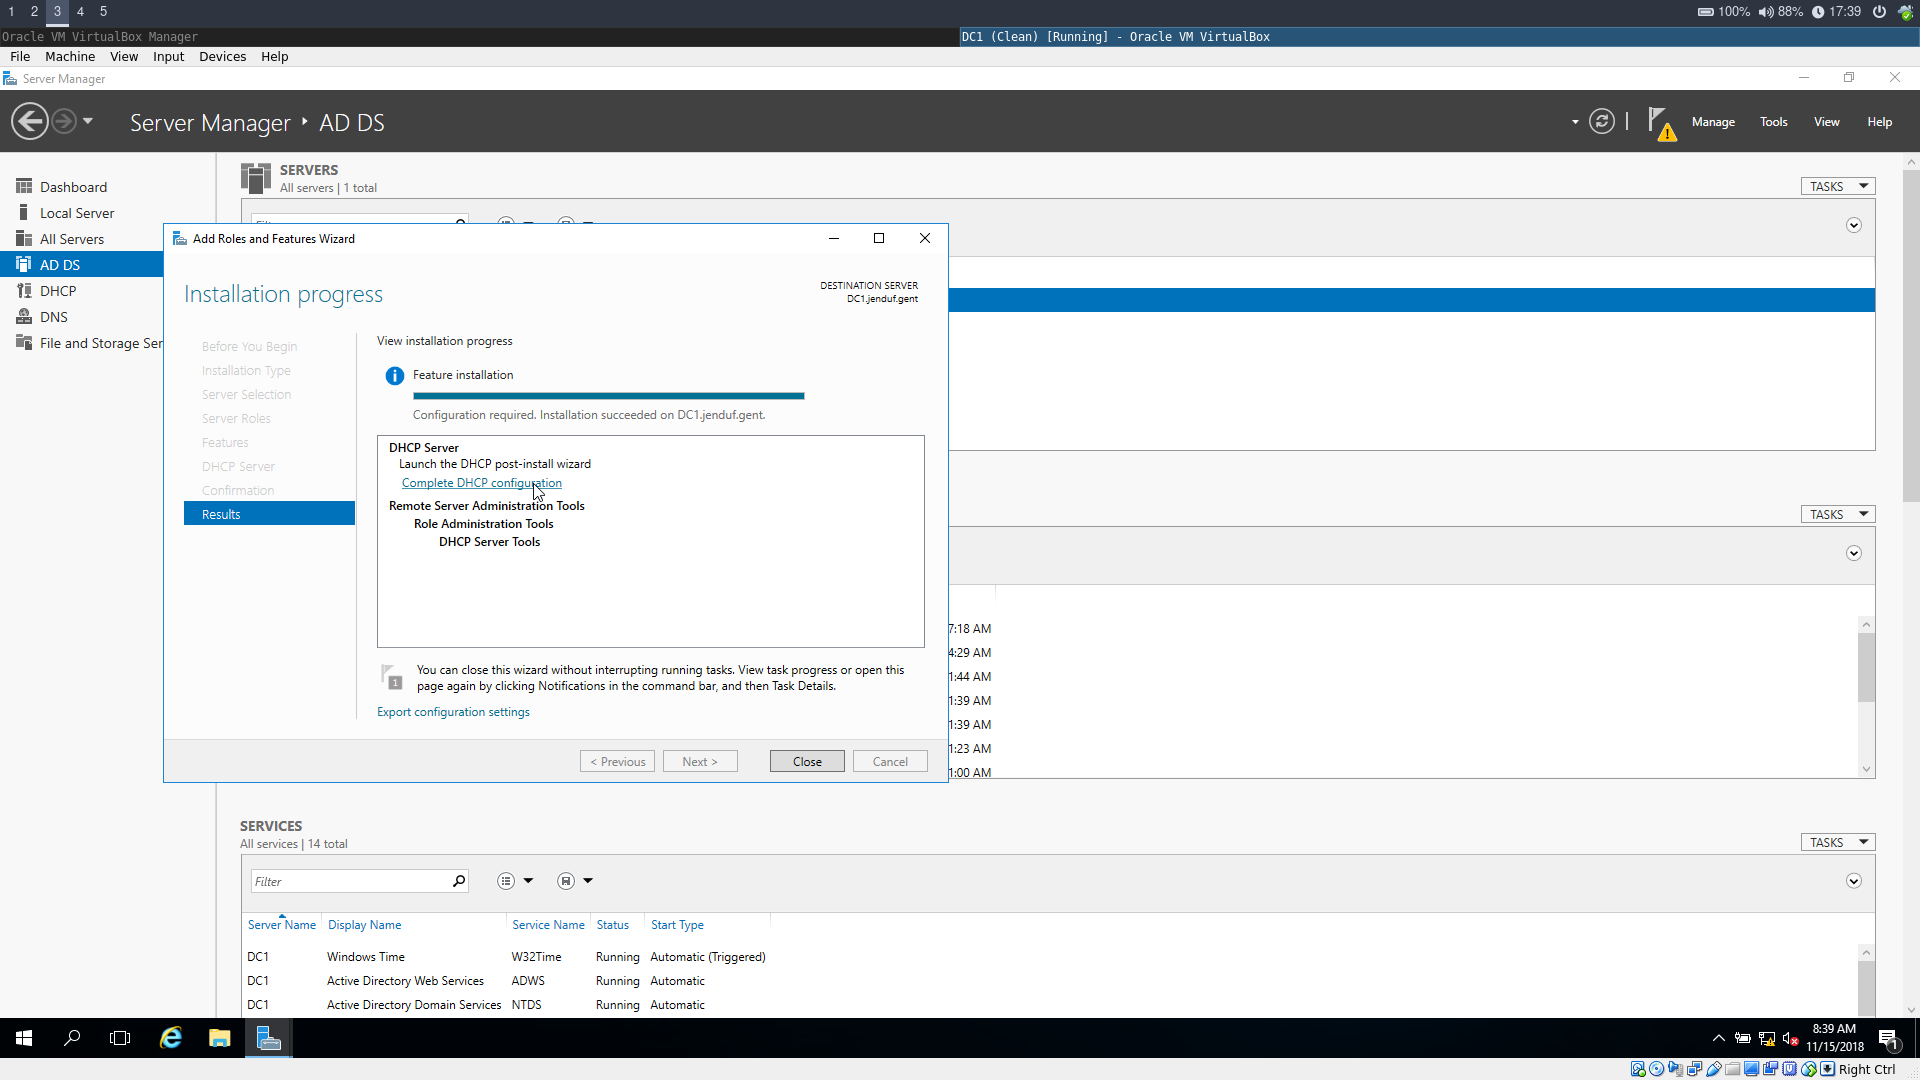
\includegraphics[width=15cm]{Pictures/DC1/DHCP/1542299953.png}
	
	Klik door naar de configuratiewizard.
\end{center}
\begin{center}
	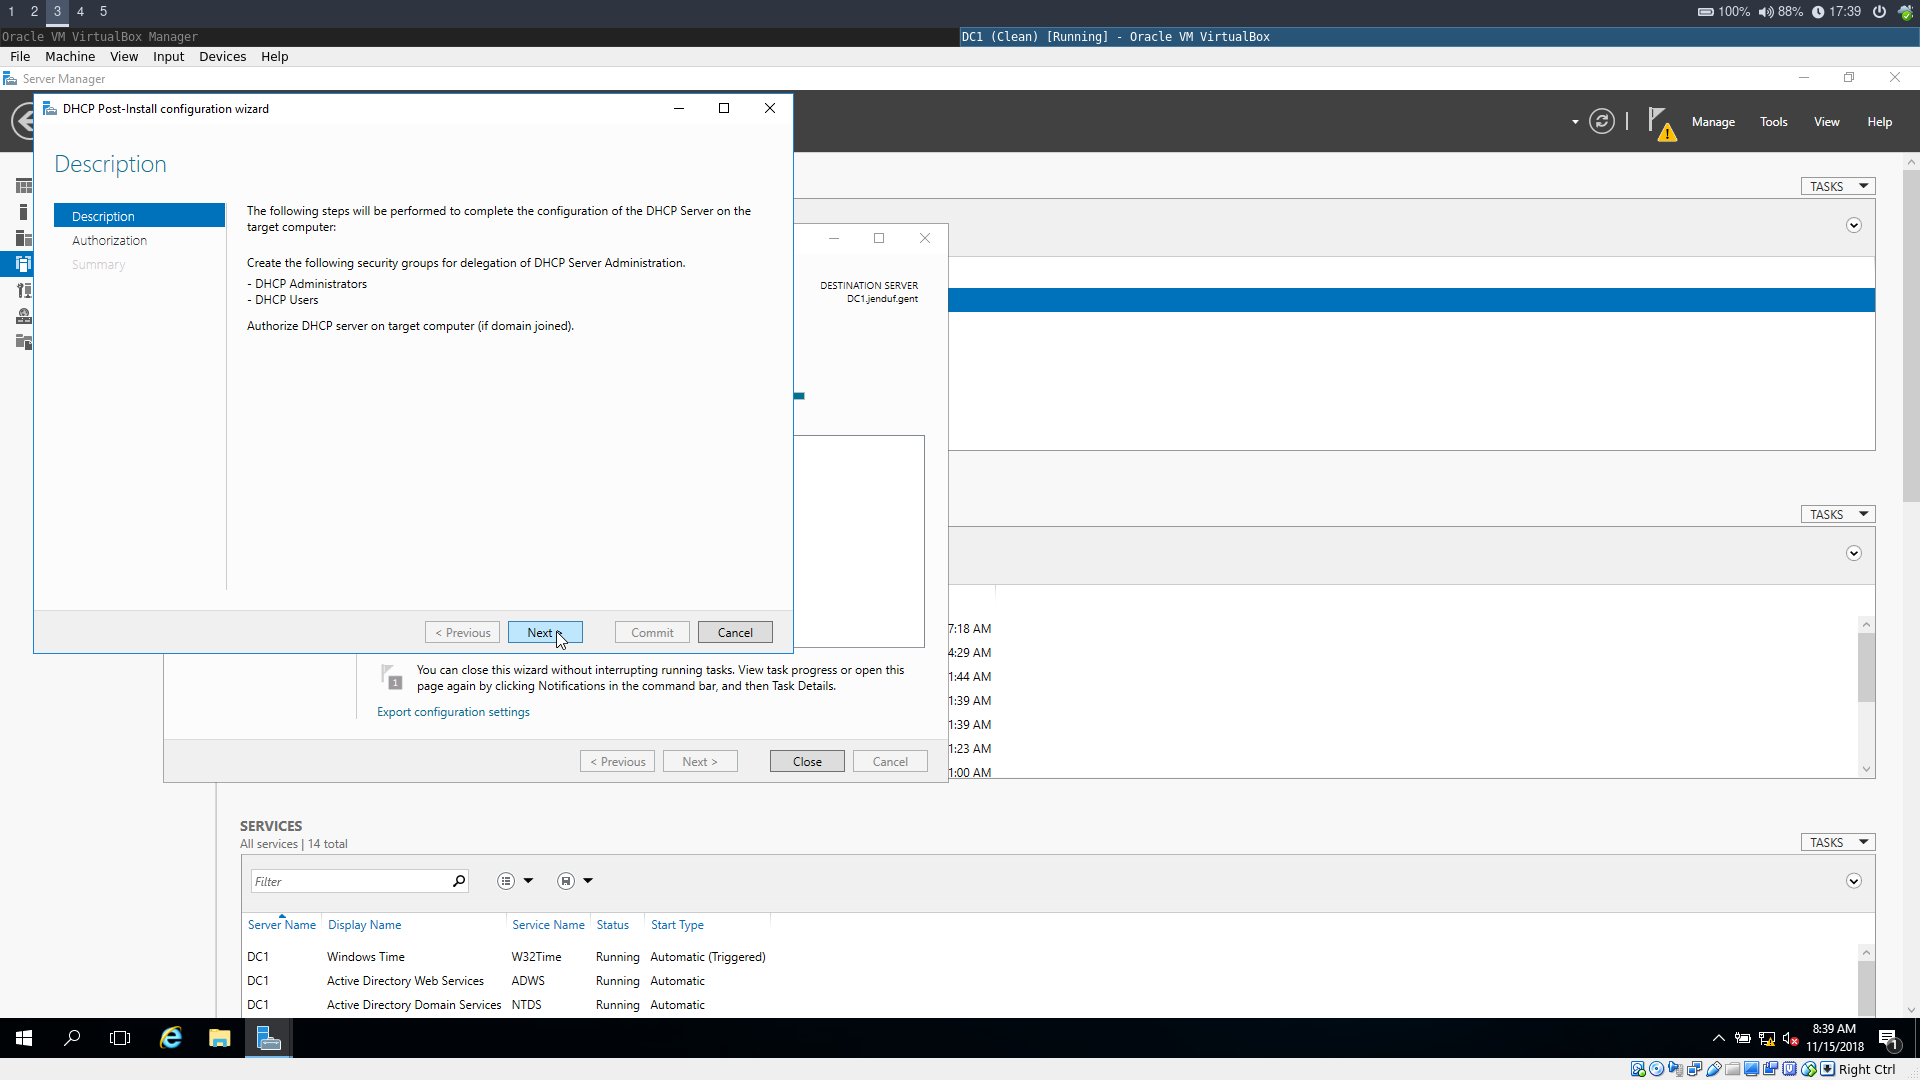
\includegraphics[width=15cm]{Pictures/DC1/DHCP/1542299964.png}
\end{center}
\begin{center}
	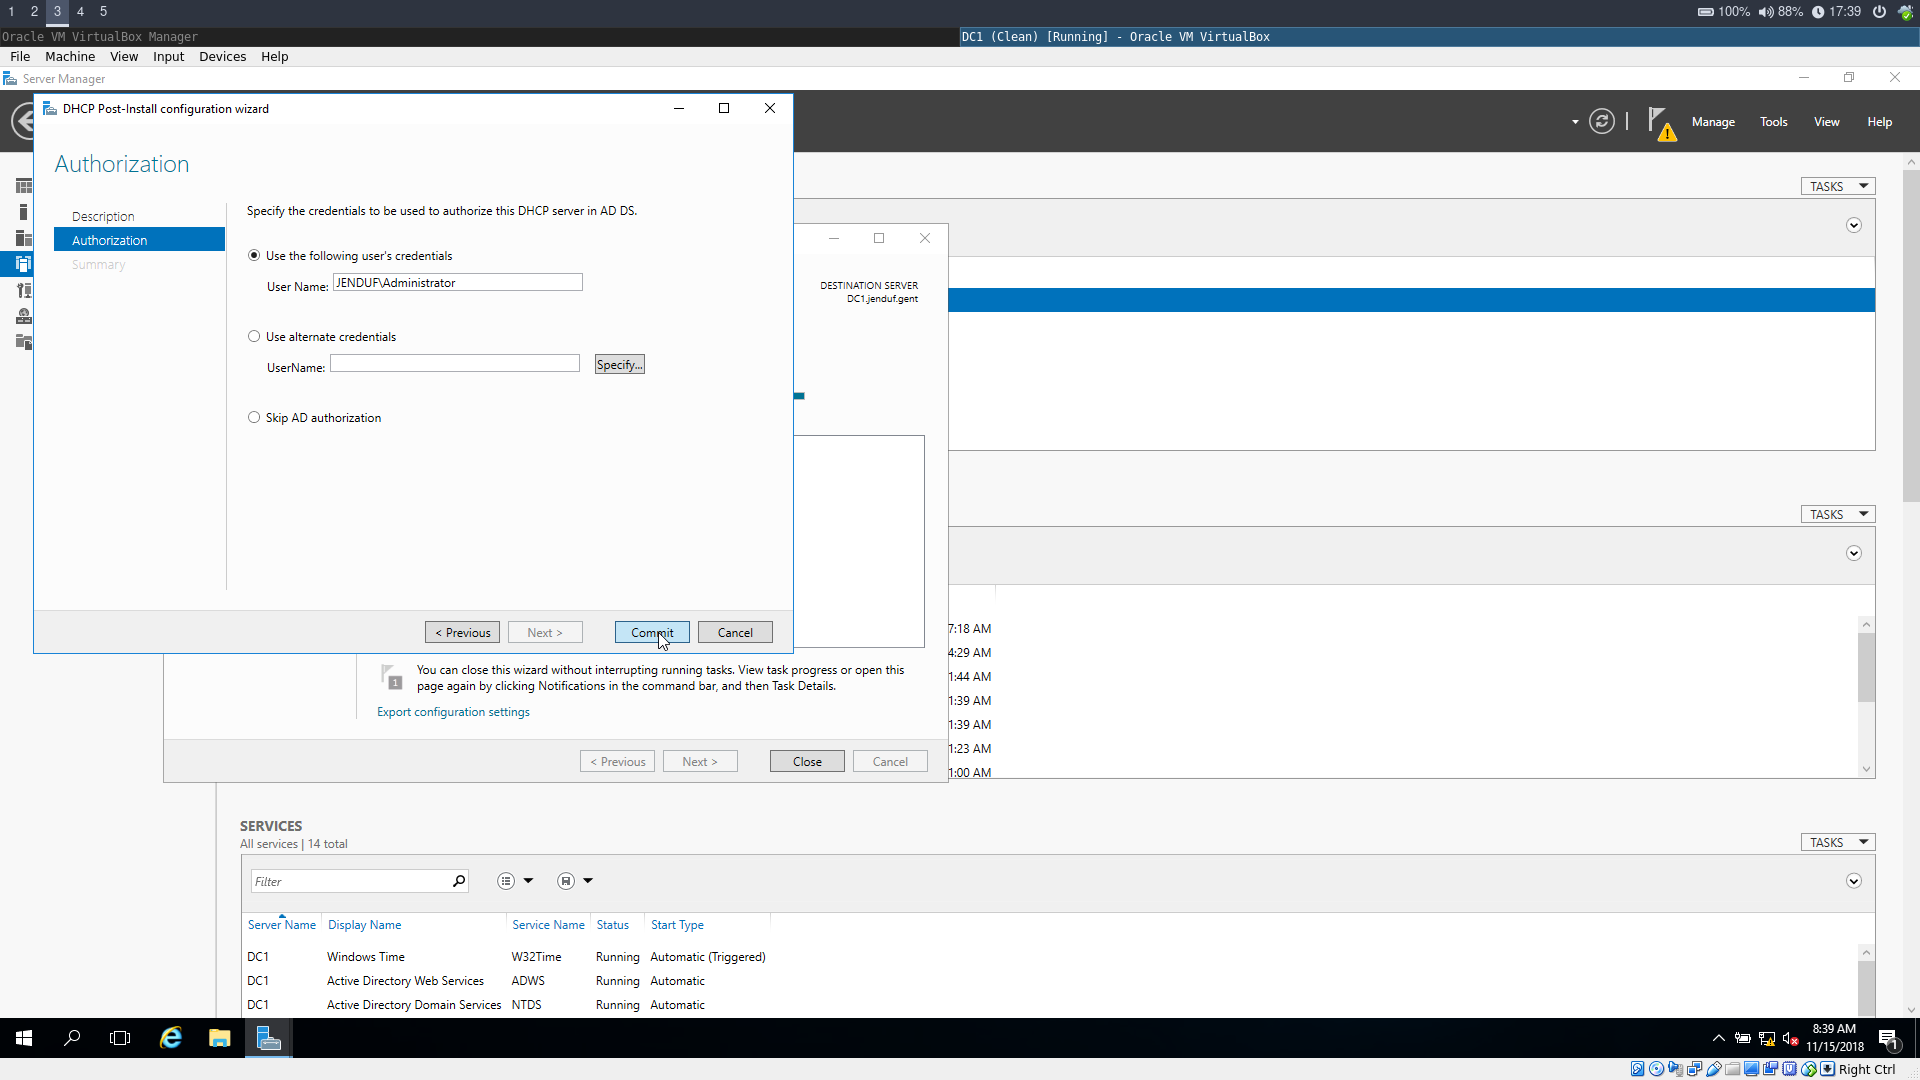
\includegraphics[width=15cm]{Pictures/DC1/DHCP/1542299973.png}
\end{center}
\begin{center}
	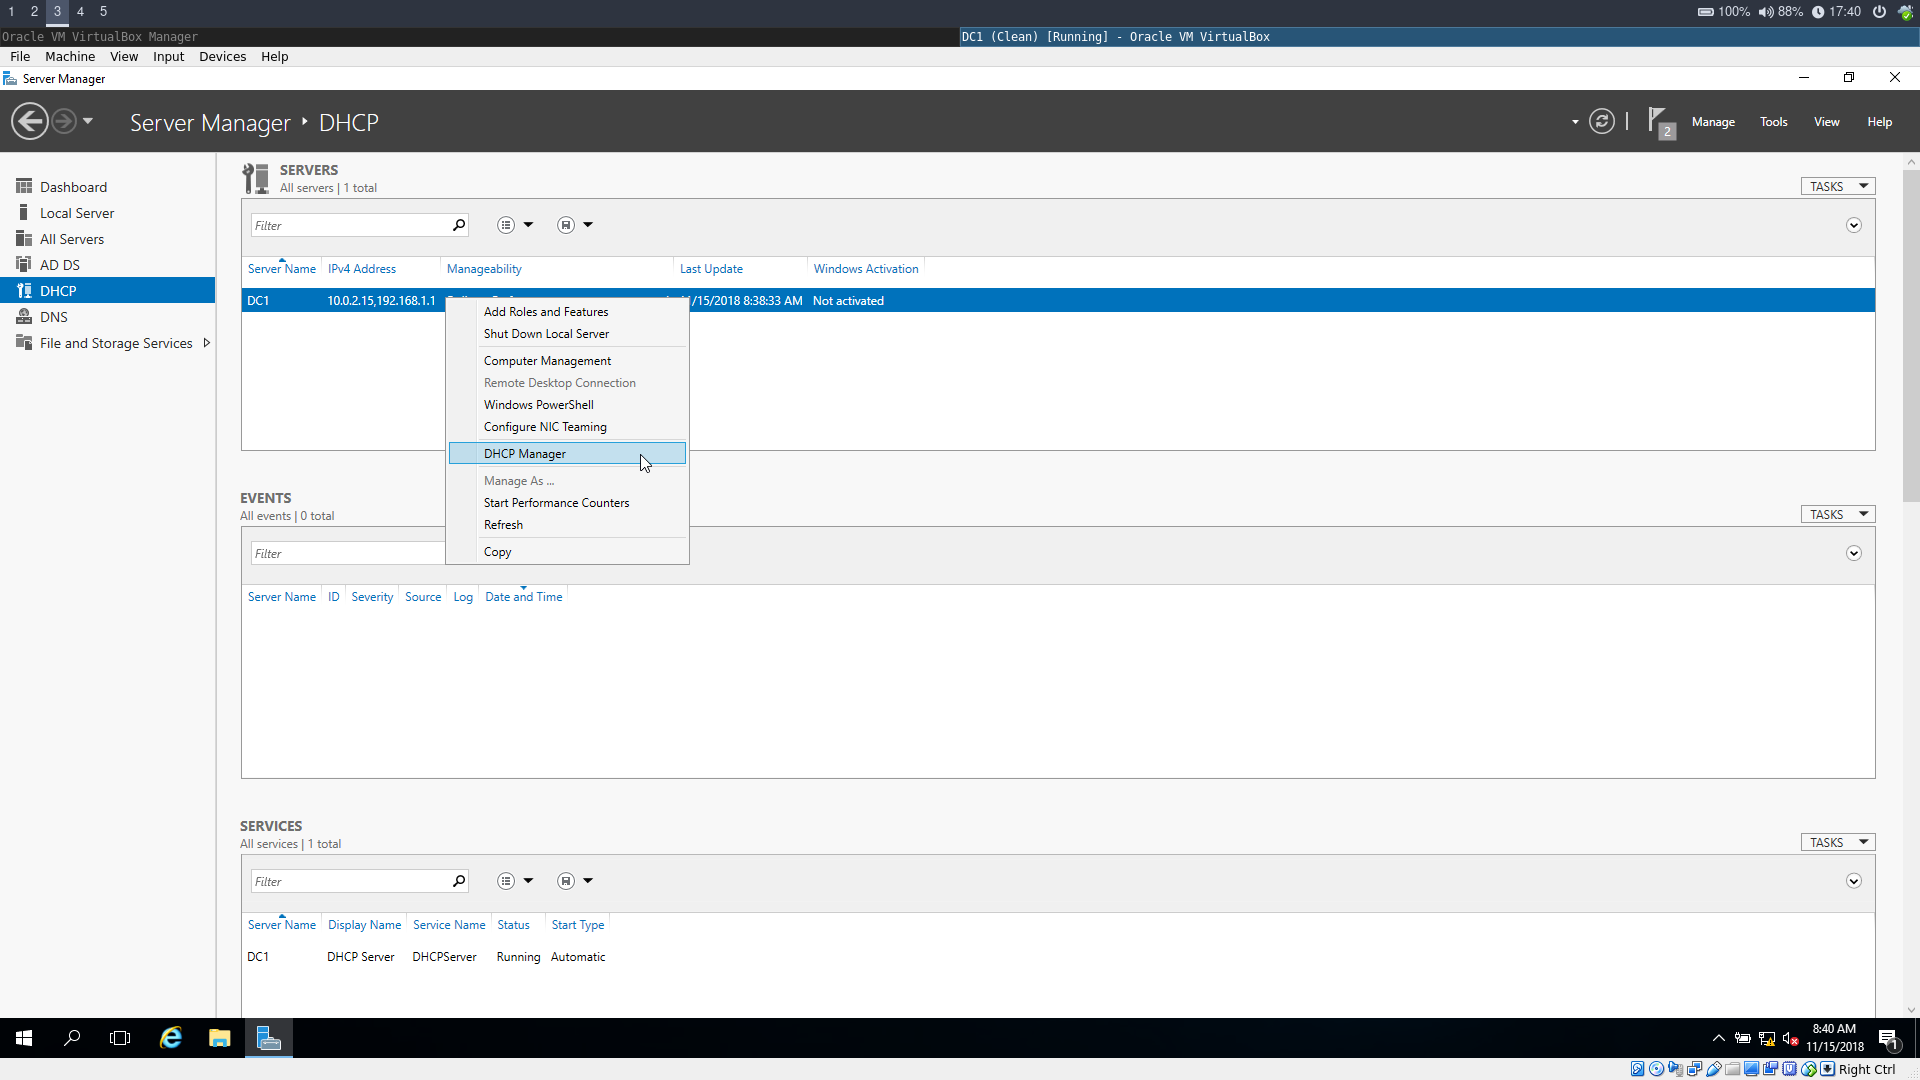
\includegraphics[width=15cm]{Pictures/DC1/DHCP/1542300003.png}
	
	Open de DHCP Manager
\end{center}
\begin{center}
	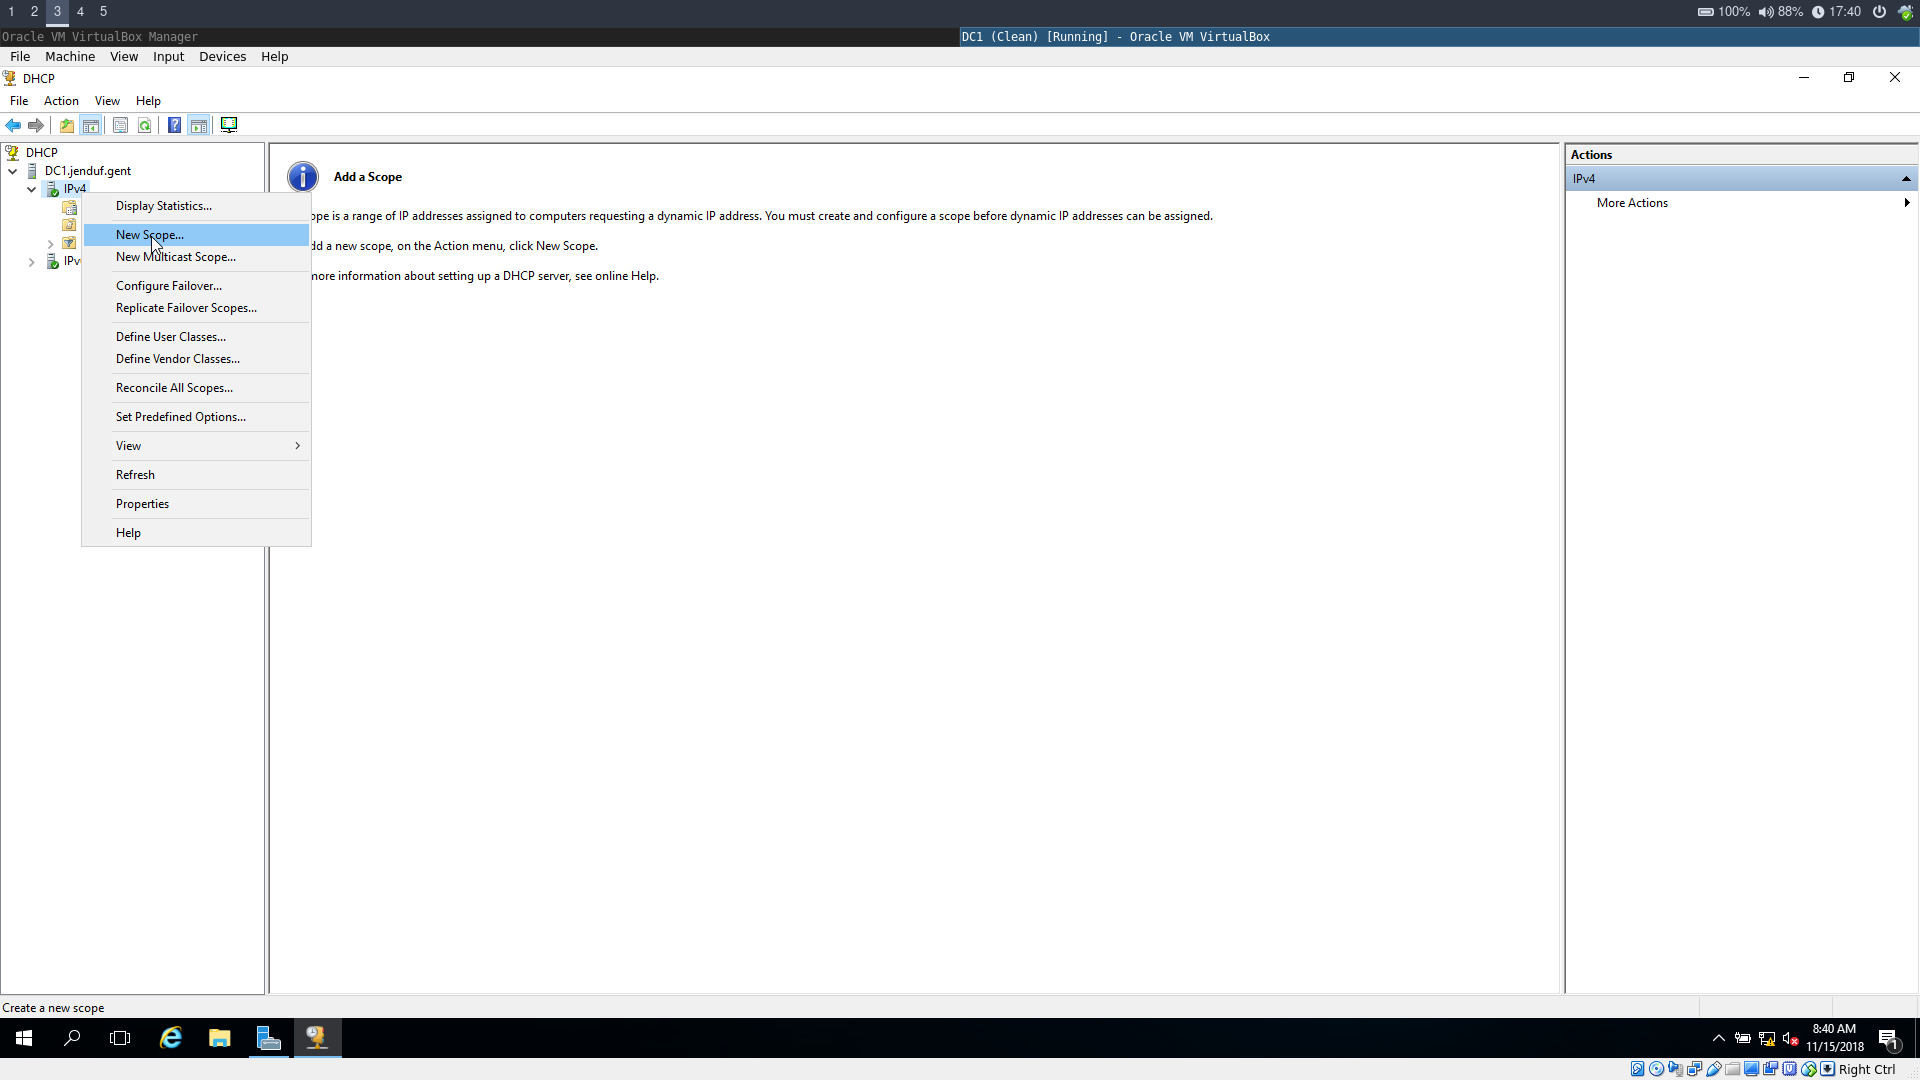
\includegraphics[width=15cm]{Pictures/DC1/DHCP/1542300021.png}
	
	Voeg een nieuwe scope toe.
\end{center}
\begin{center}
	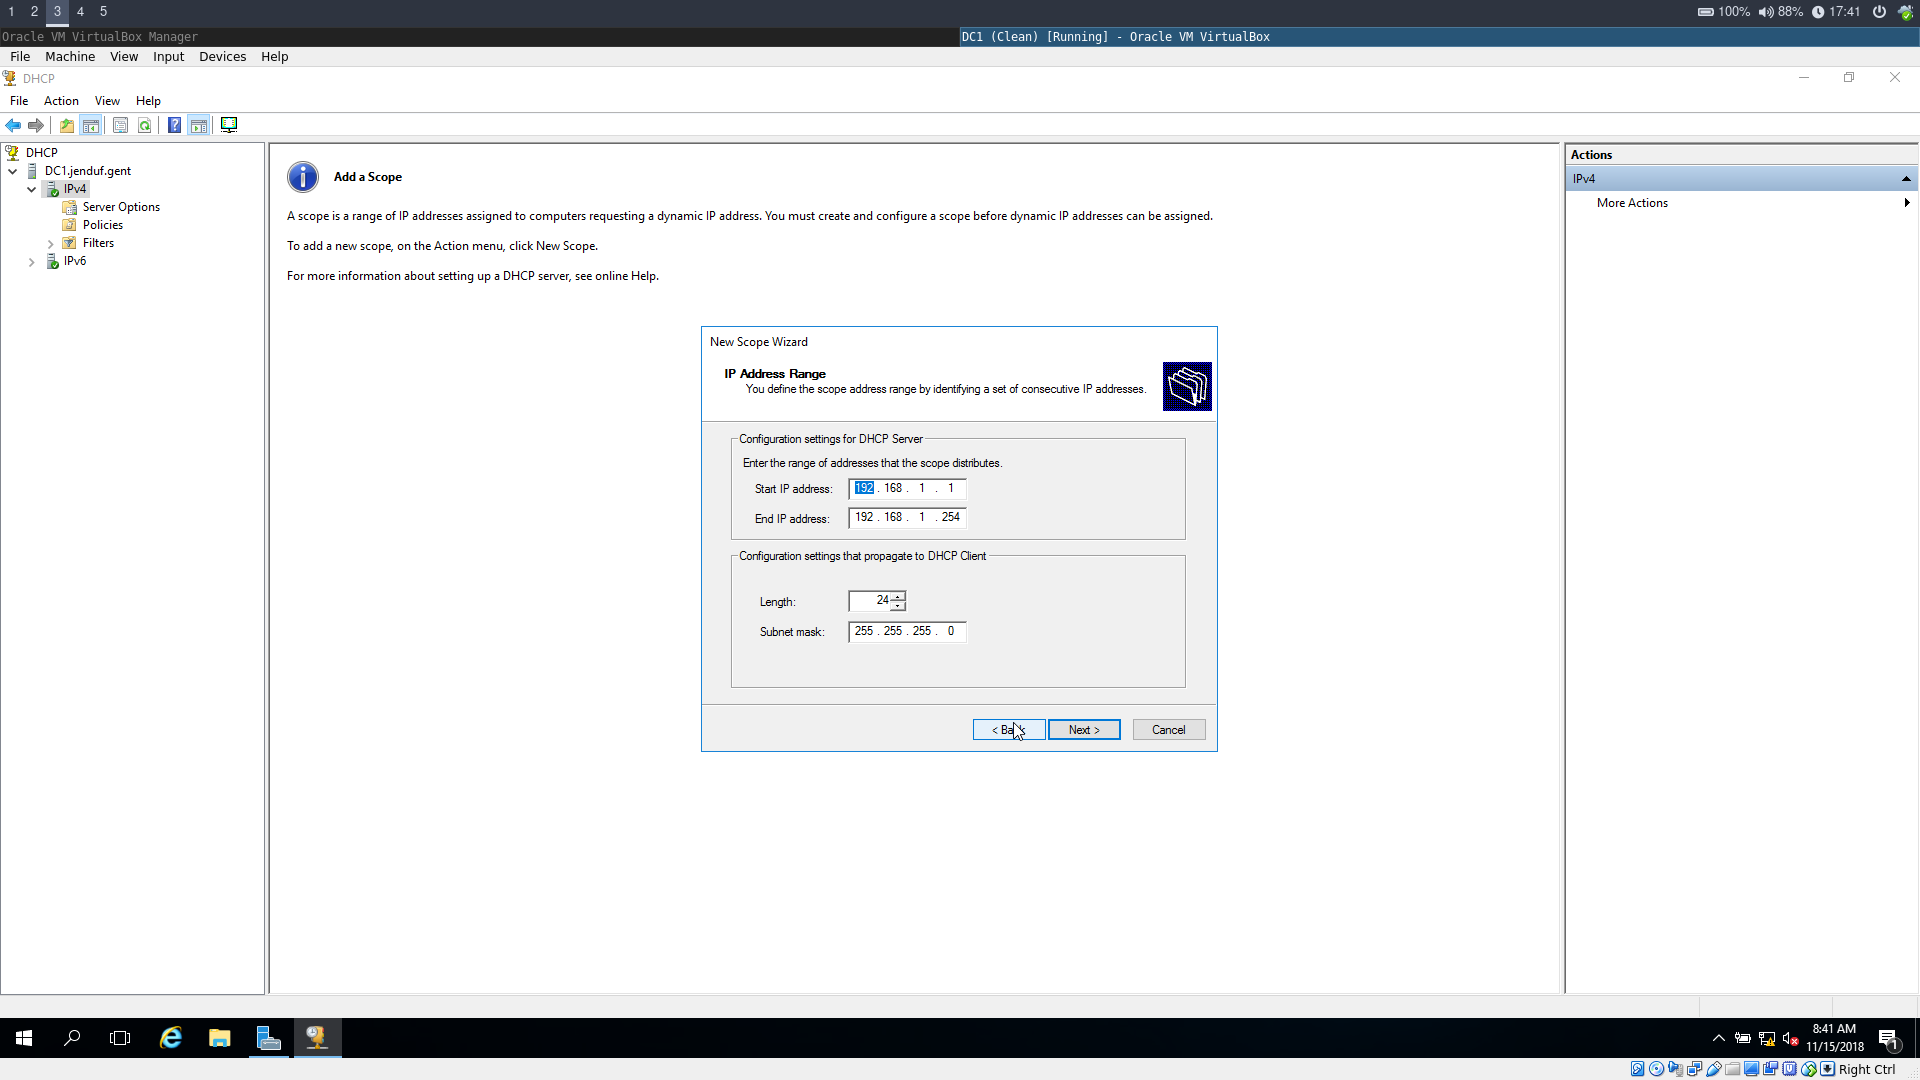
\includegraphics[width=15cm]{Pictures/DC1/DHCP/1542300063.png}
	
	Geef het addressenbereik in.
\end{center}
\begin{center}
	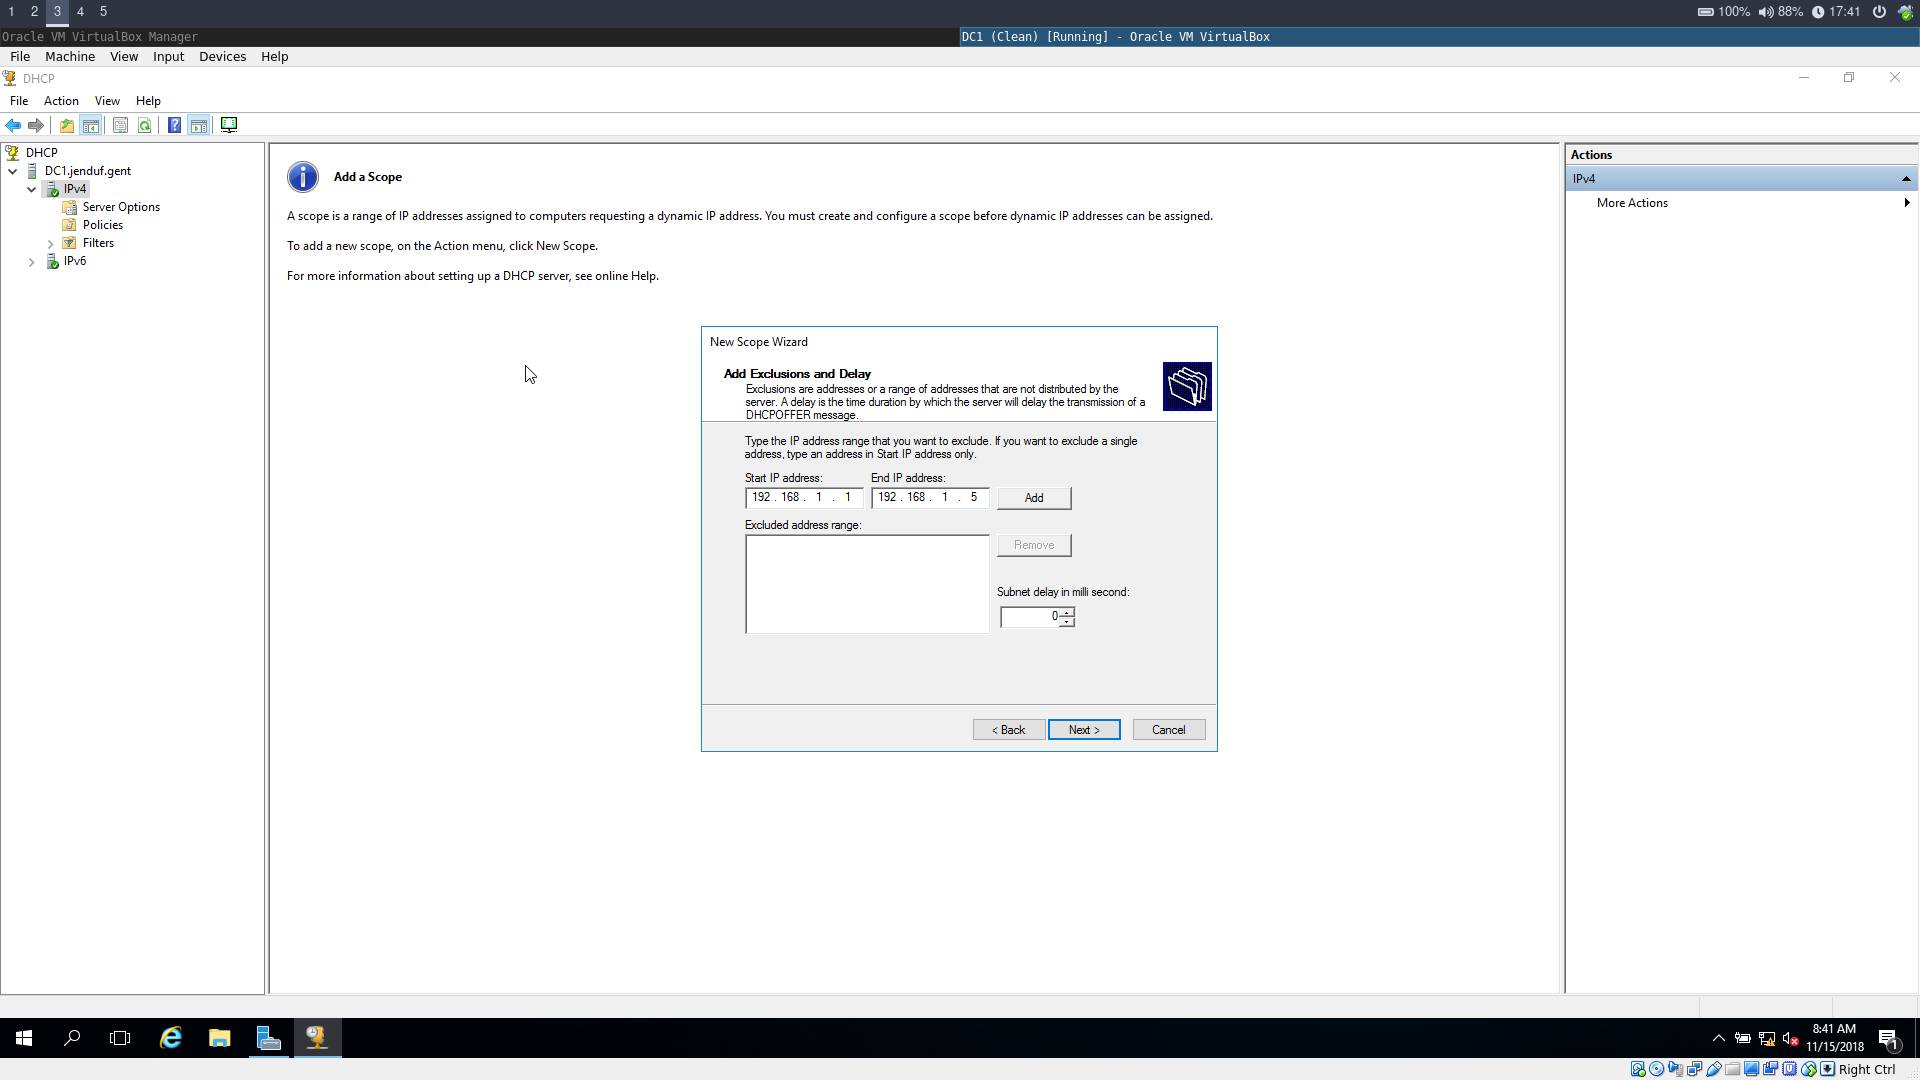
\includegraphics[width=15cm]{Pictures/DC1/DHCP/1542300111.png}
	
	Geef de uitgesloten adressen in.
\end{center}
\begin{center}
	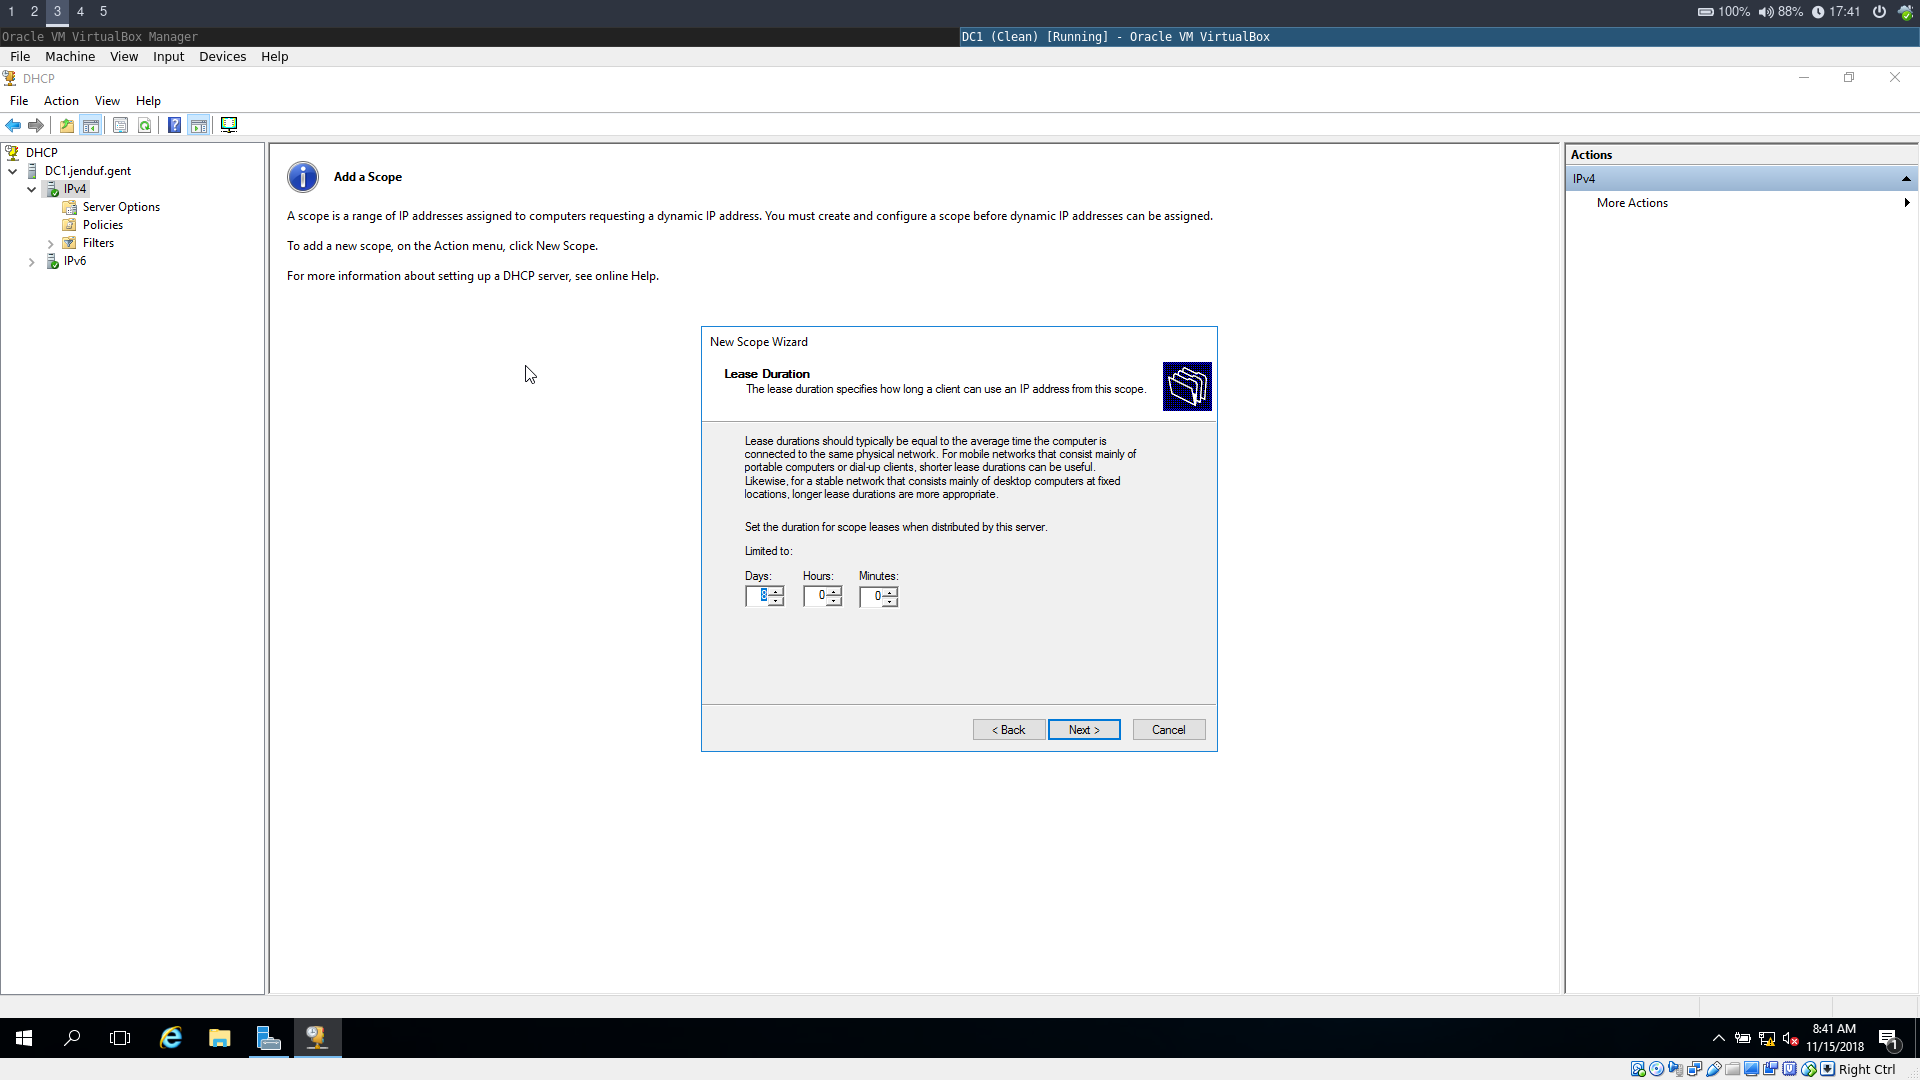
\includegraphics[width=15cm]{Pictures/DC1/DHCP/1542300114.png}
	
	Geef de levensduur in.
\end{center}
\begin{center}
	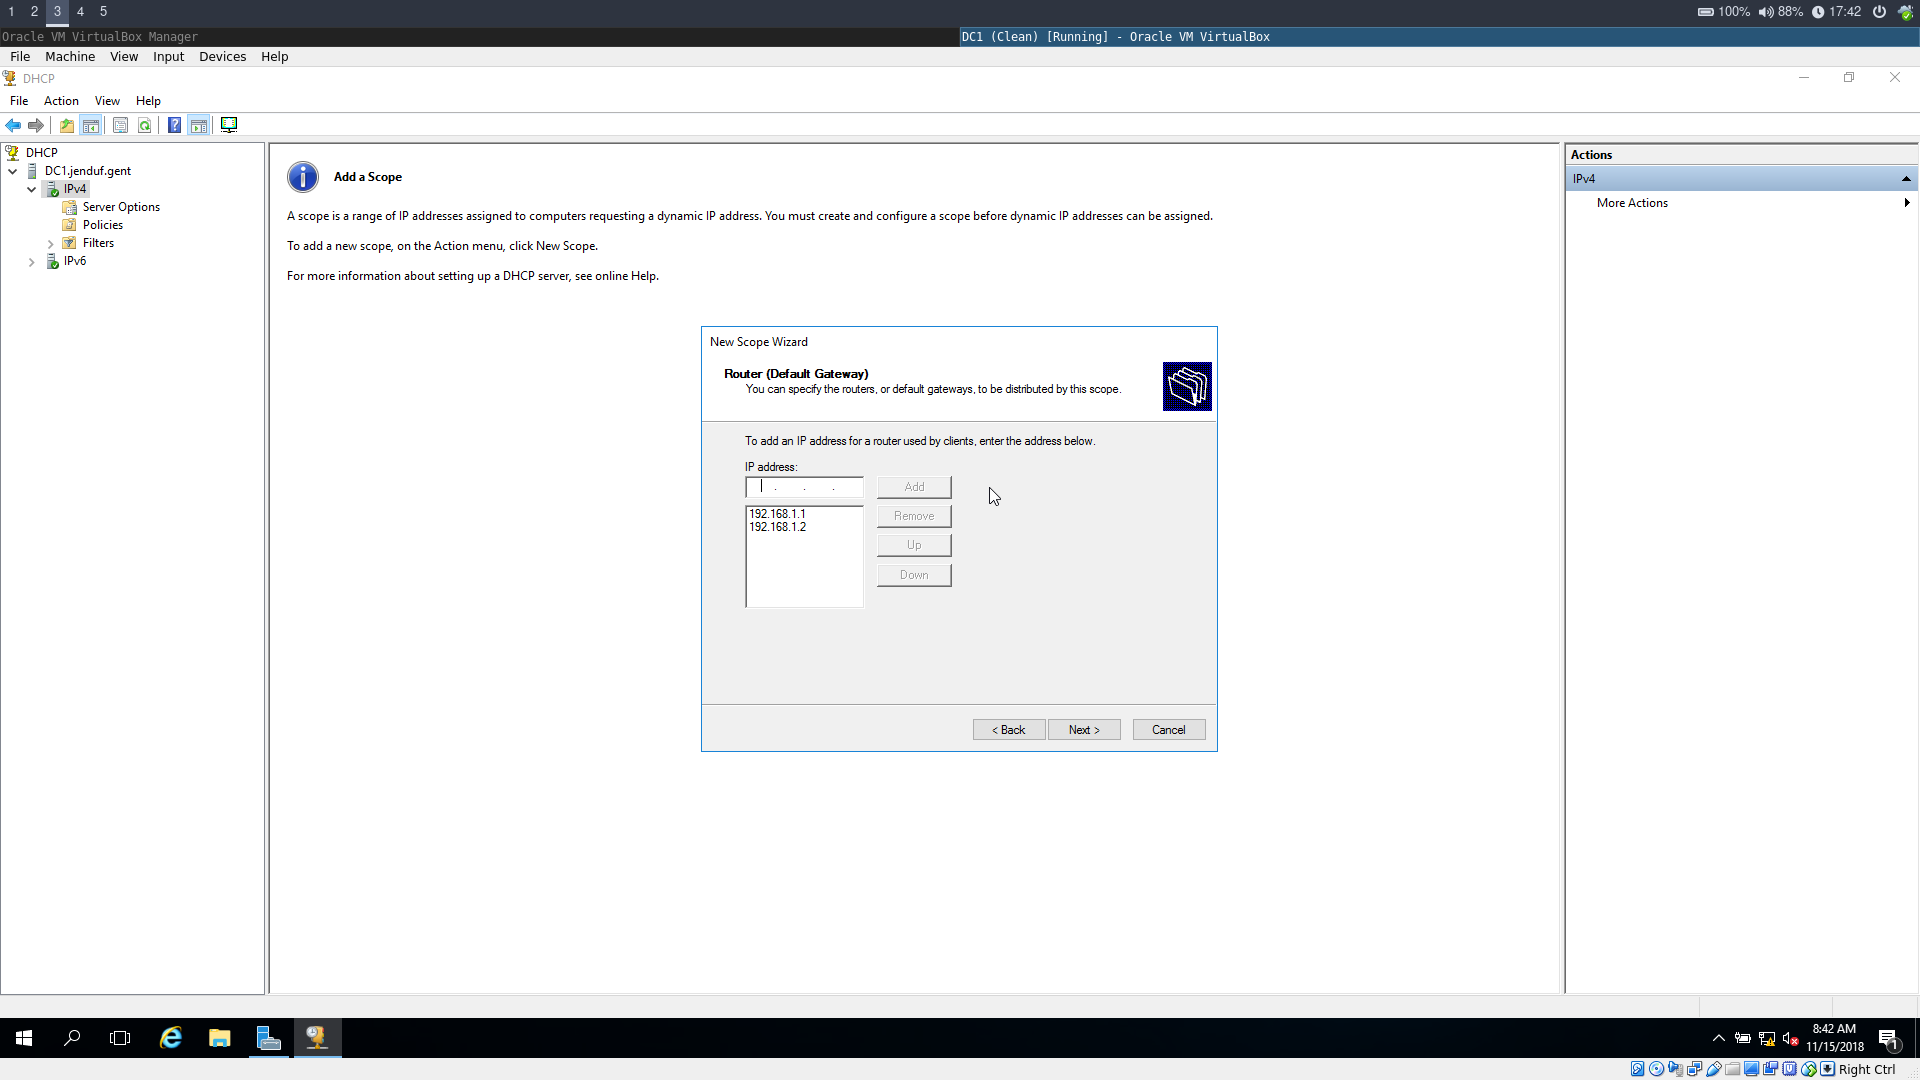
\includegraphics[width=15cm]{Pictures/DC1/DHCP/1542300144.png}
	
	Geef de IP addressen in van DC1 en DC2.
\end{center}
\begin{center}
	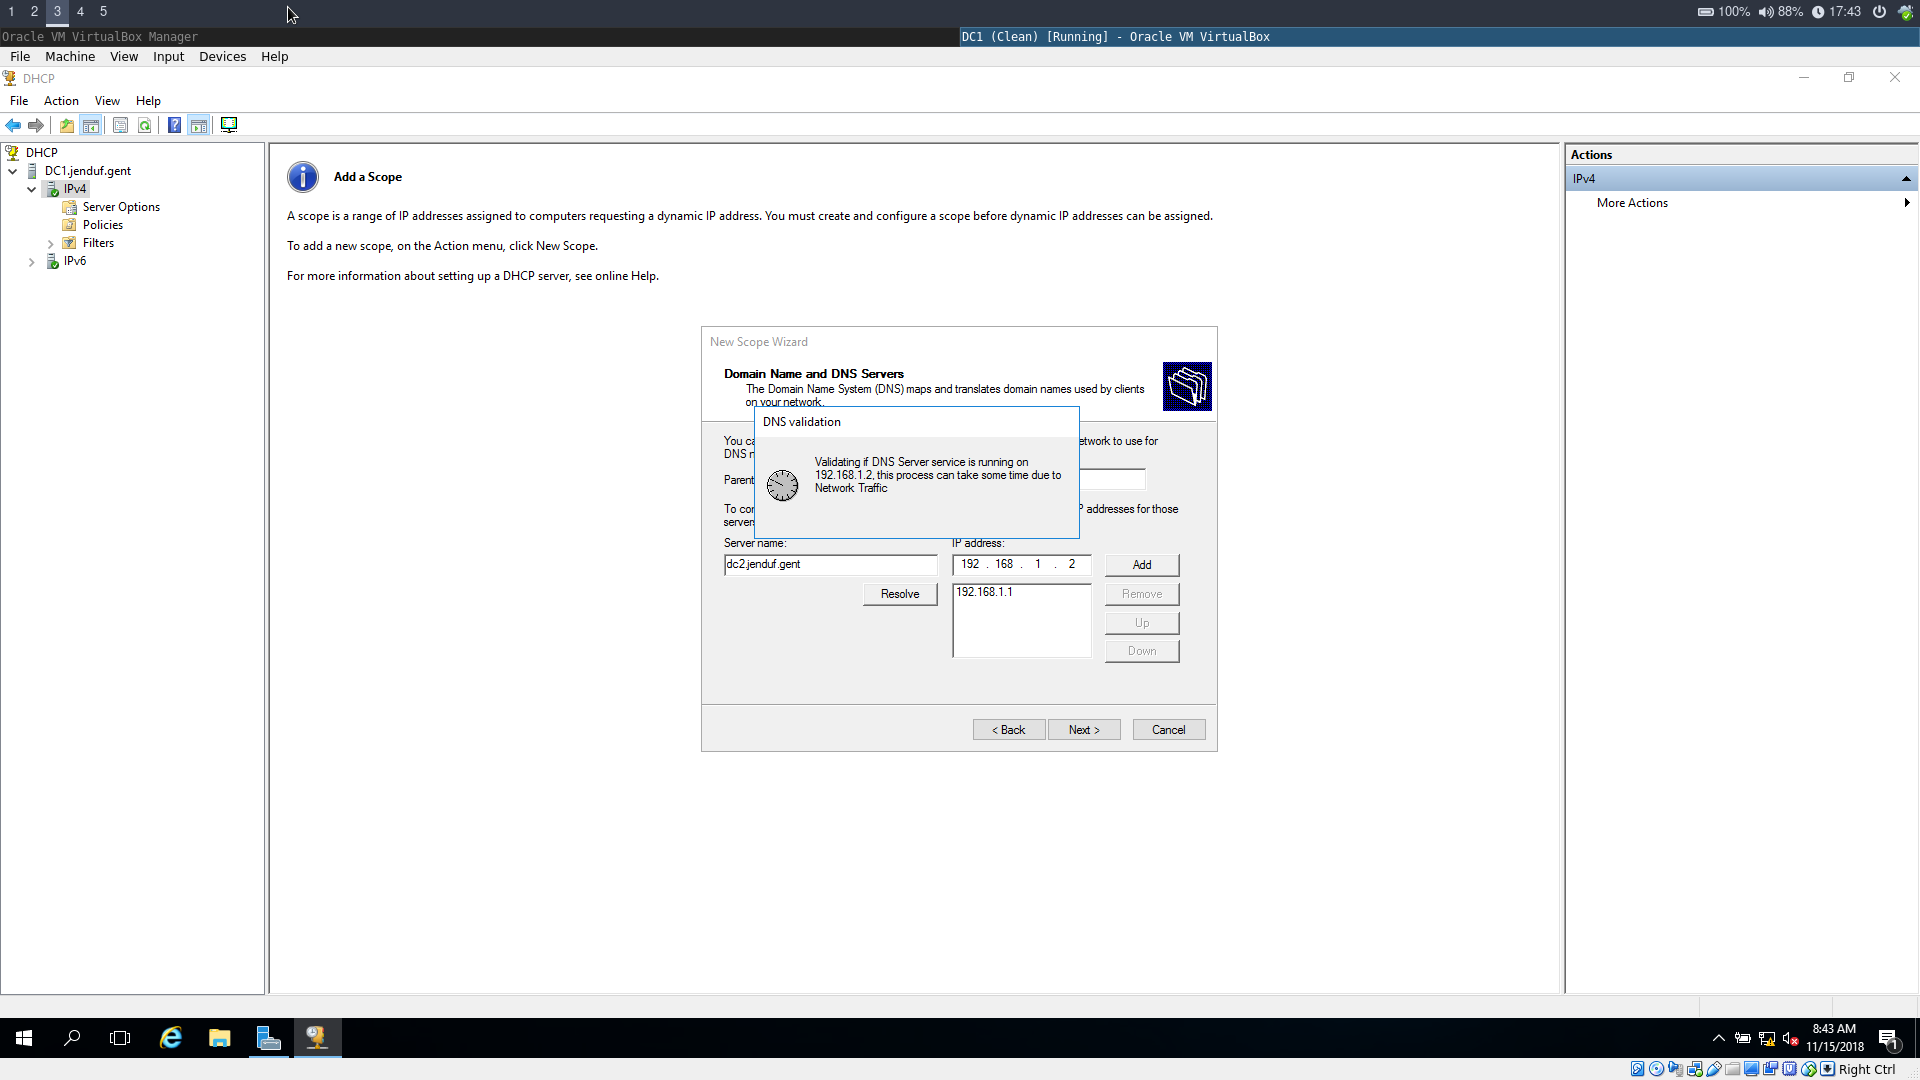
\includegraphics[width=15cm]{Pictures/DC1/DHCP/1542300195.png}
	
	Geef de IP addressen in van DC1 en DC2 gelinkt aan hun naam voor de DNS.	
\end{center}
\begin{center}
	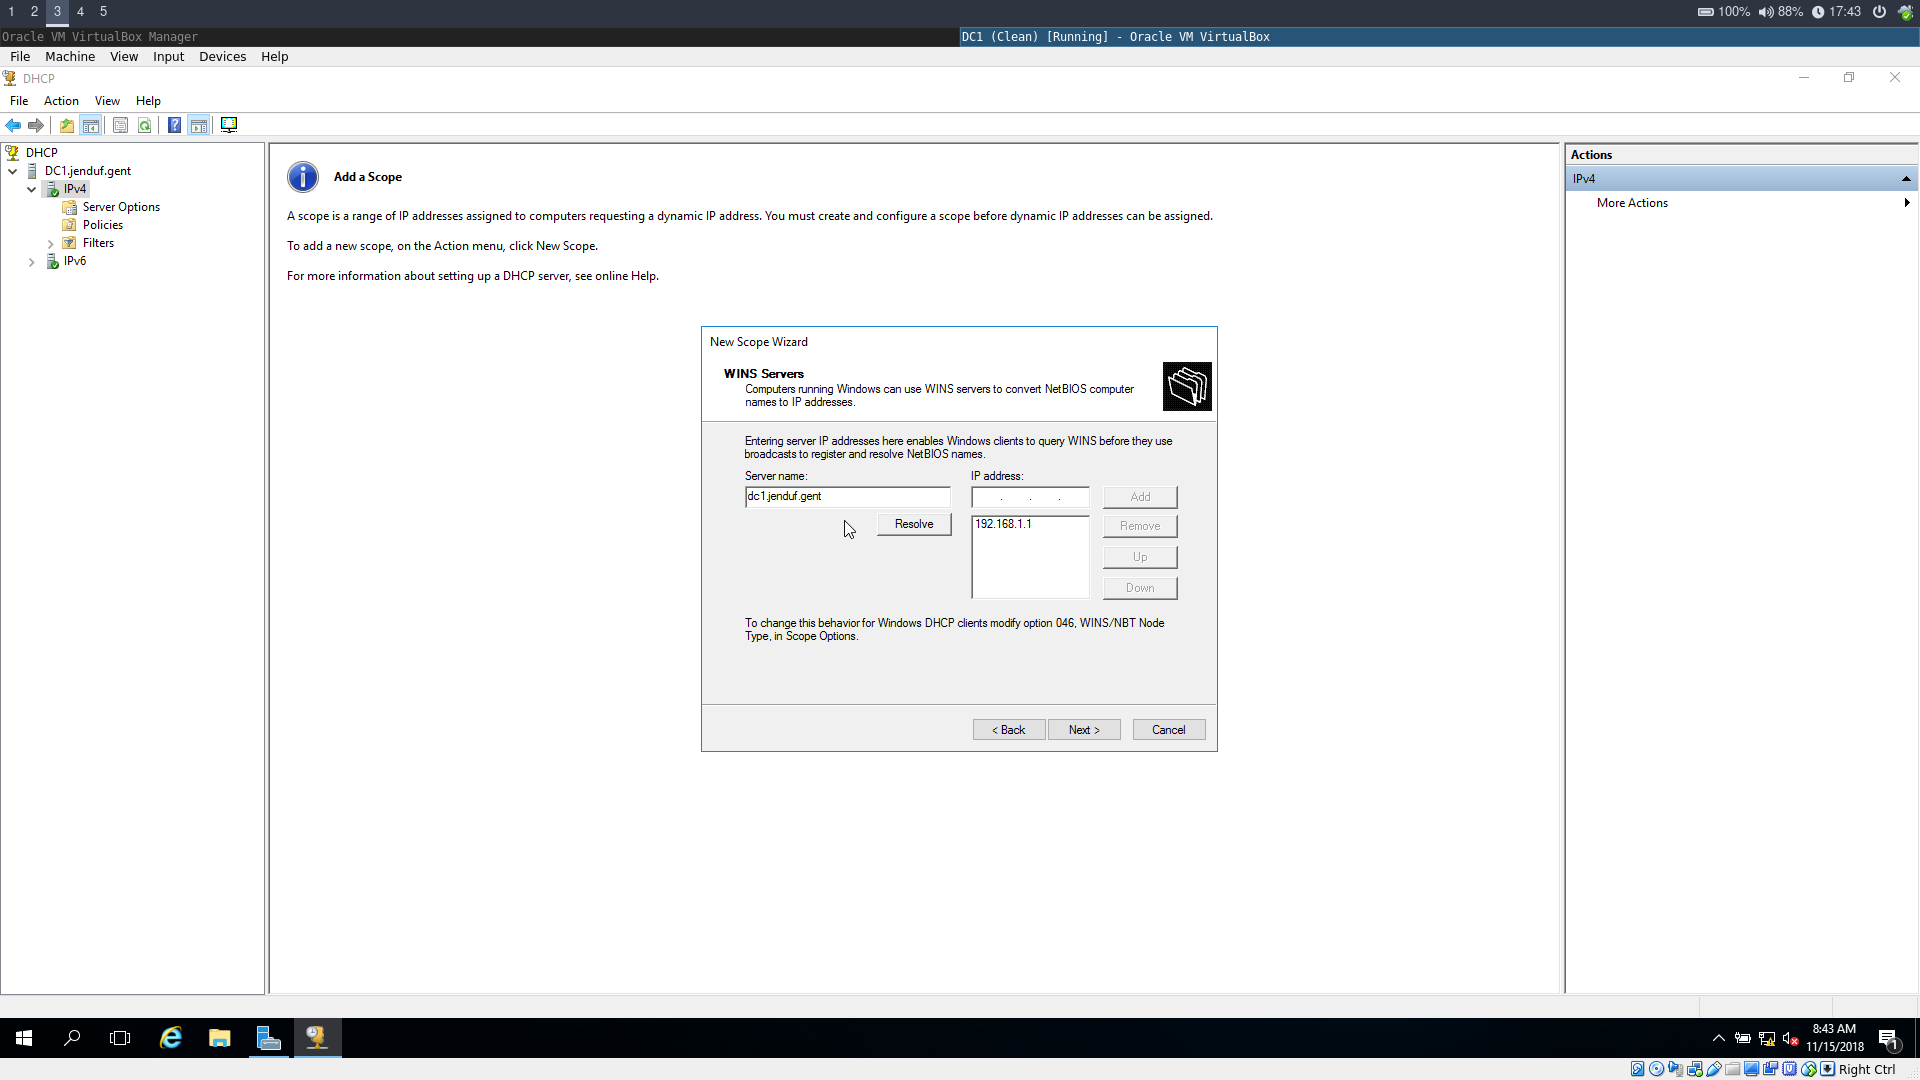
\includegraphics[width=15cm]{Pictures/DC1/DHCP/1542300229.png}
	
	Geef de IP addressen in van DC1 en DC2 gelinkt aan hun naam voor de WINS Servers.	
\end{center}
\begin{center}
	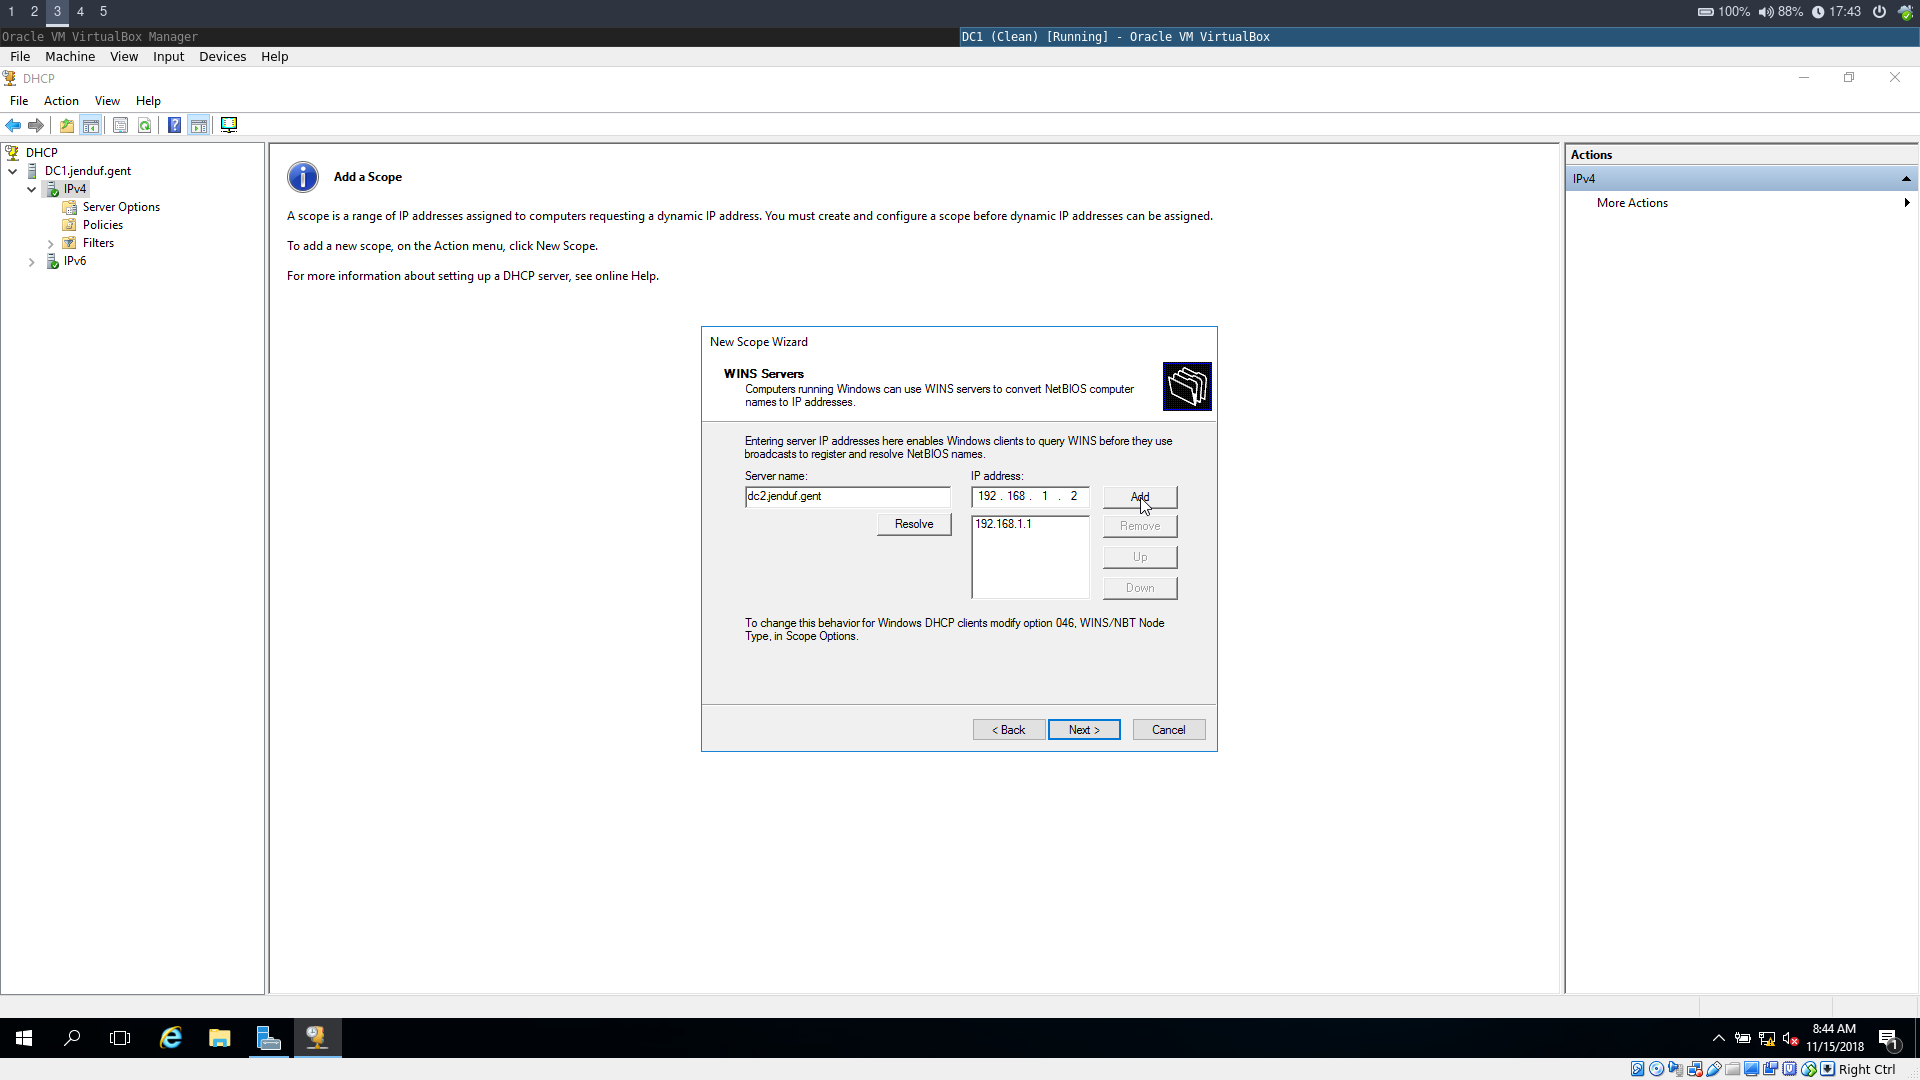
\includegraphics[width=15cm]{Pictures/DC1/DHCP/1542300240.png}
\end{center}
\begin{center}
	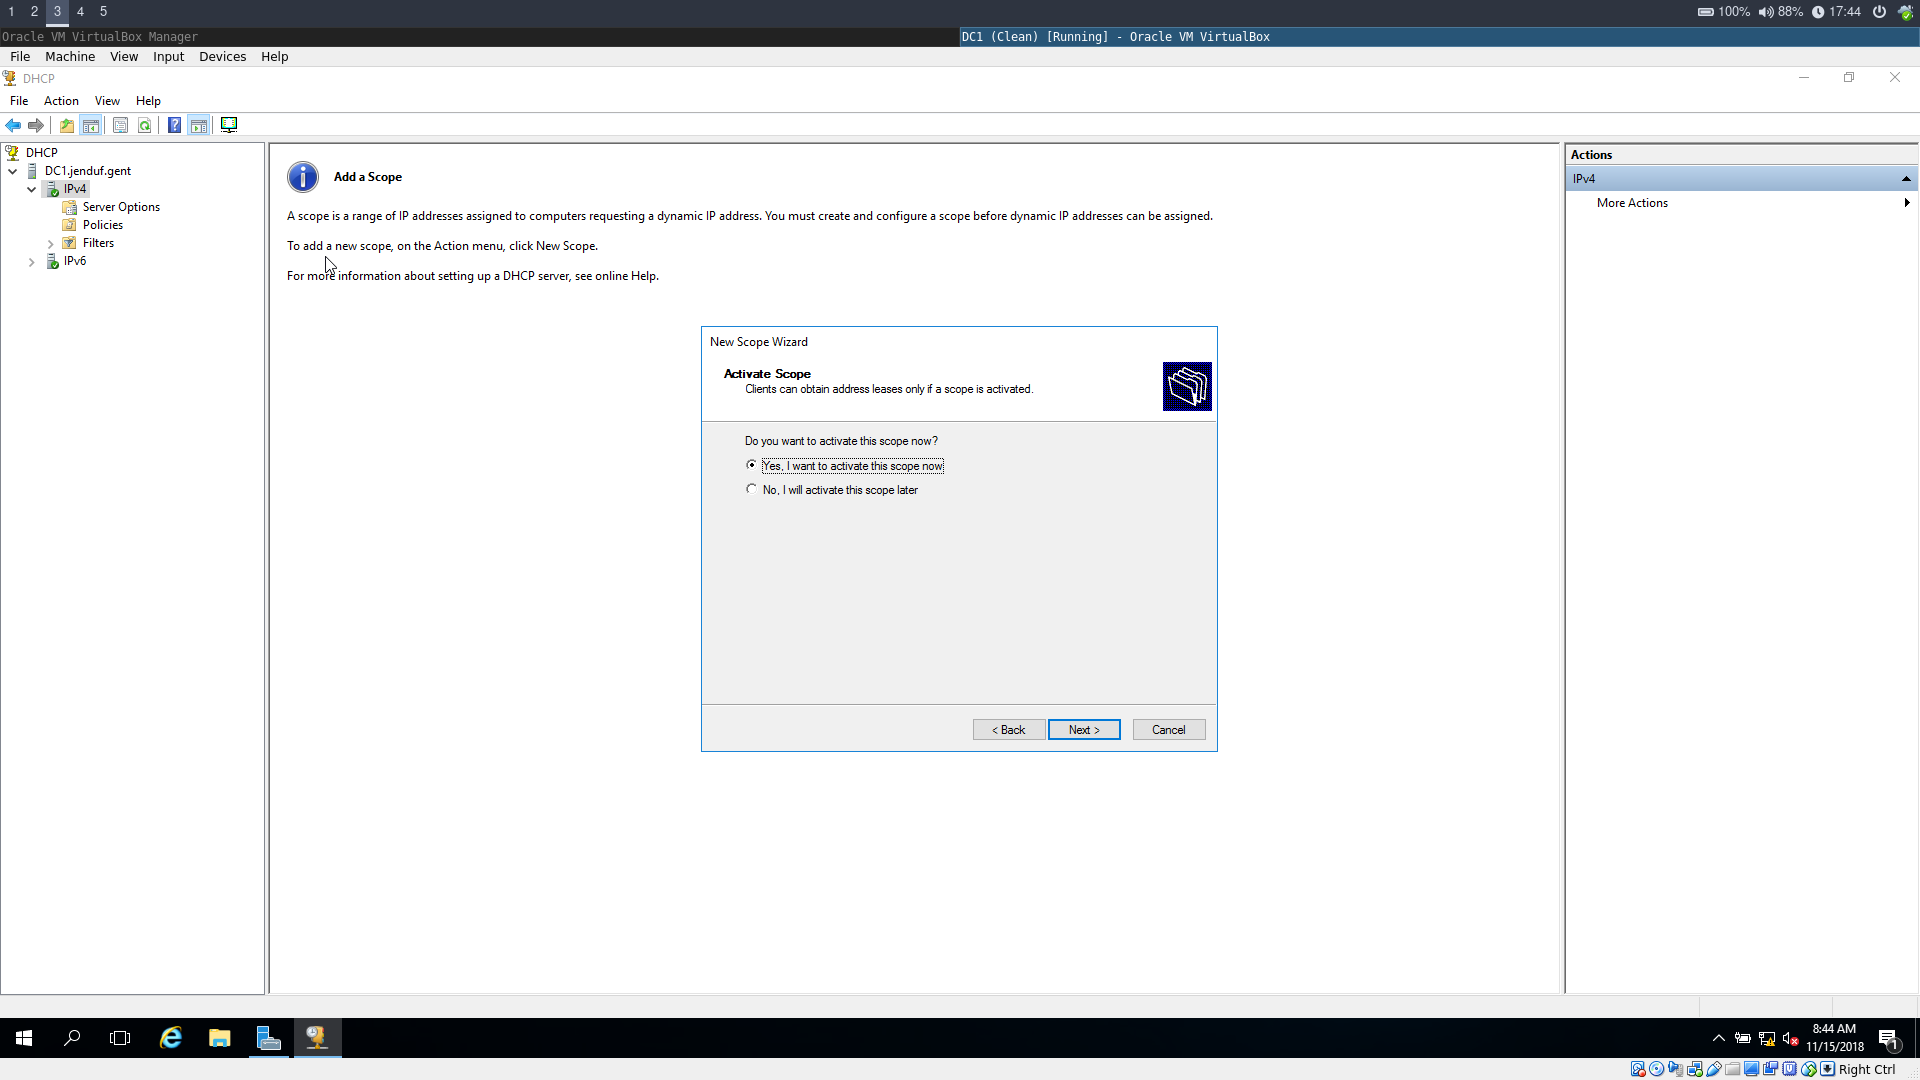
\includegraphics[width=15cm]{Pictures/DC1/DHCP/1542300248.png}
	
	Activeer de nieuwe scope.
\end{center}


\section{Configuratie DNS}
De DNS-service werd automatisch geïnstalleerd met de ADDS.
\section{Configuratie Routing}
\begin{center}
	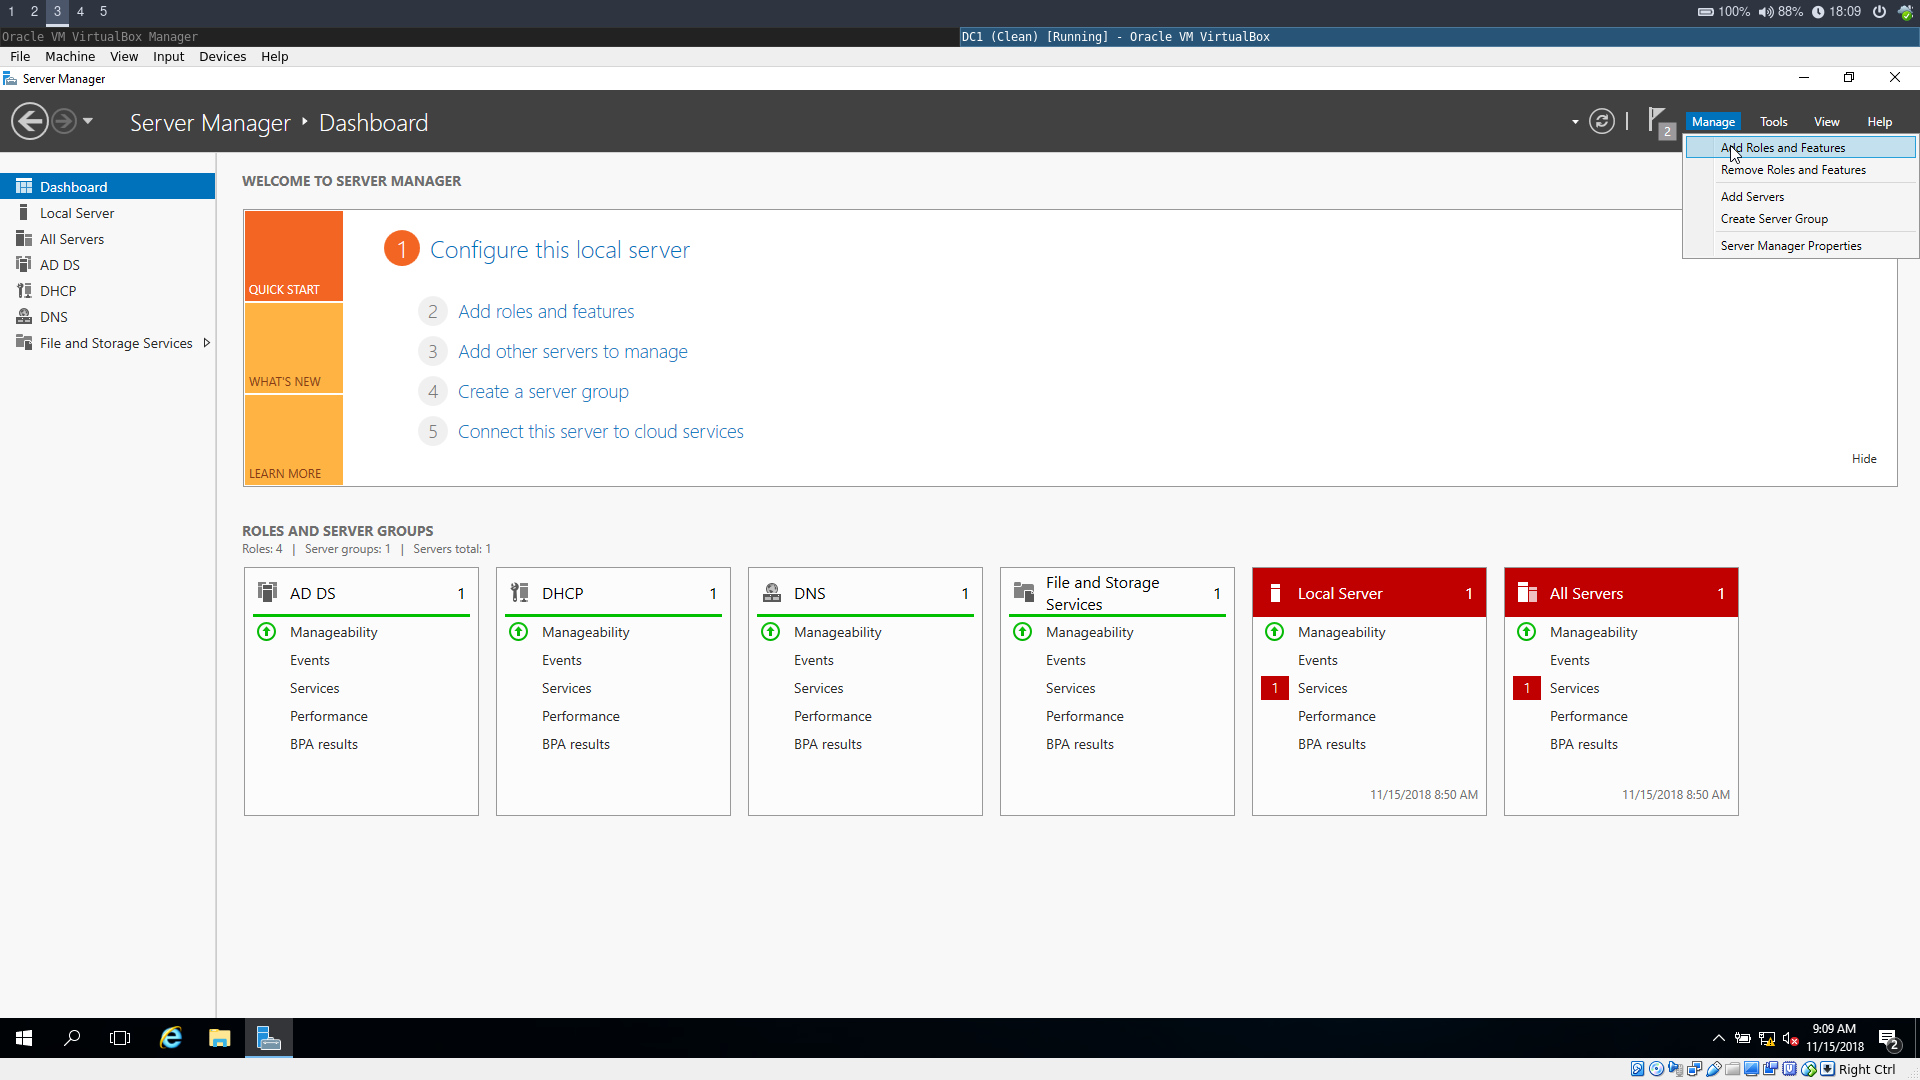
\includegraphics[width=15cm]{Pictures/DC1/Routing/1542301791.png}
\end{center}
\begin{center}
	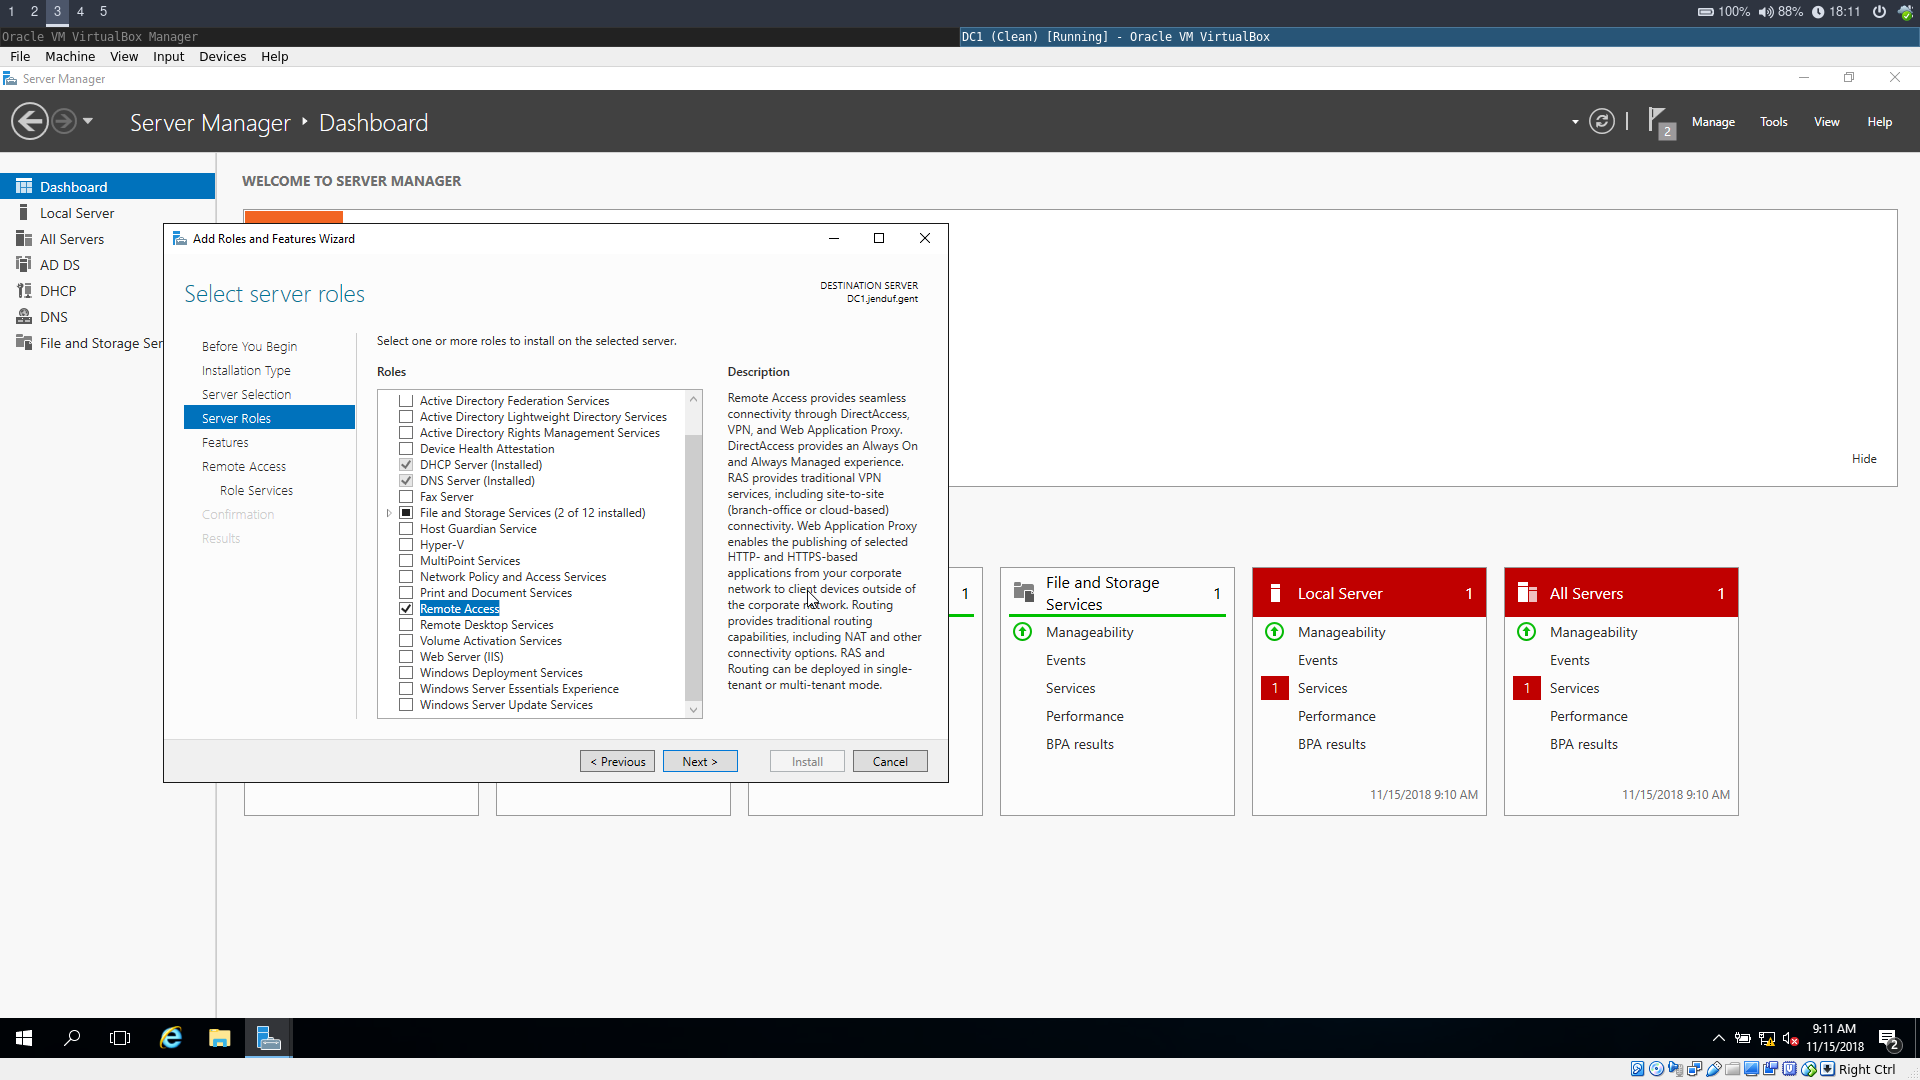
\includegraphics[width=15cm]{Pictures/DC1/Routing/1542301906.png}
	
	Voeg de rol "Remote Access" toe.
\end{center}
\begin{center}
	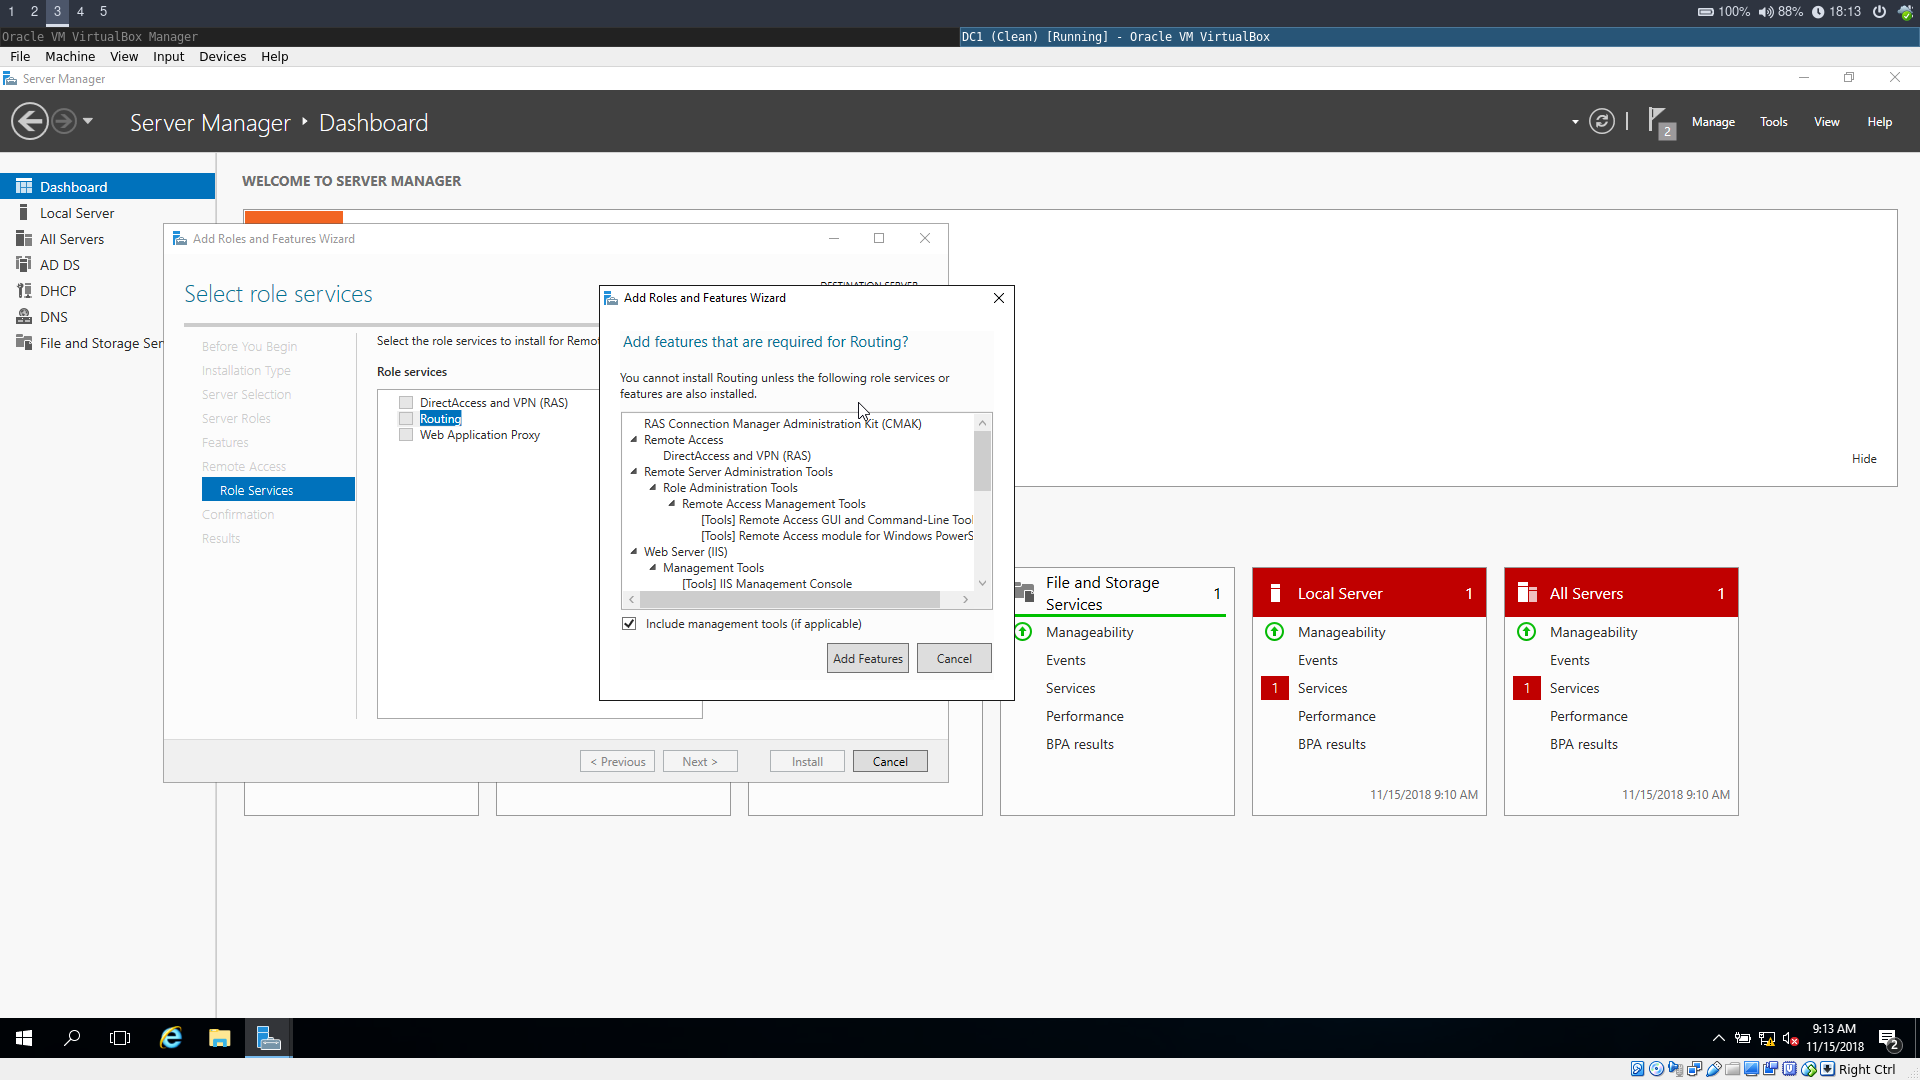
\includegraphics[width=15cm]{Pictures/DC1/Routing/1542301993.png}
	
	Selecteer Routing als installatie-optie.
\end{center}
\begin{center}
	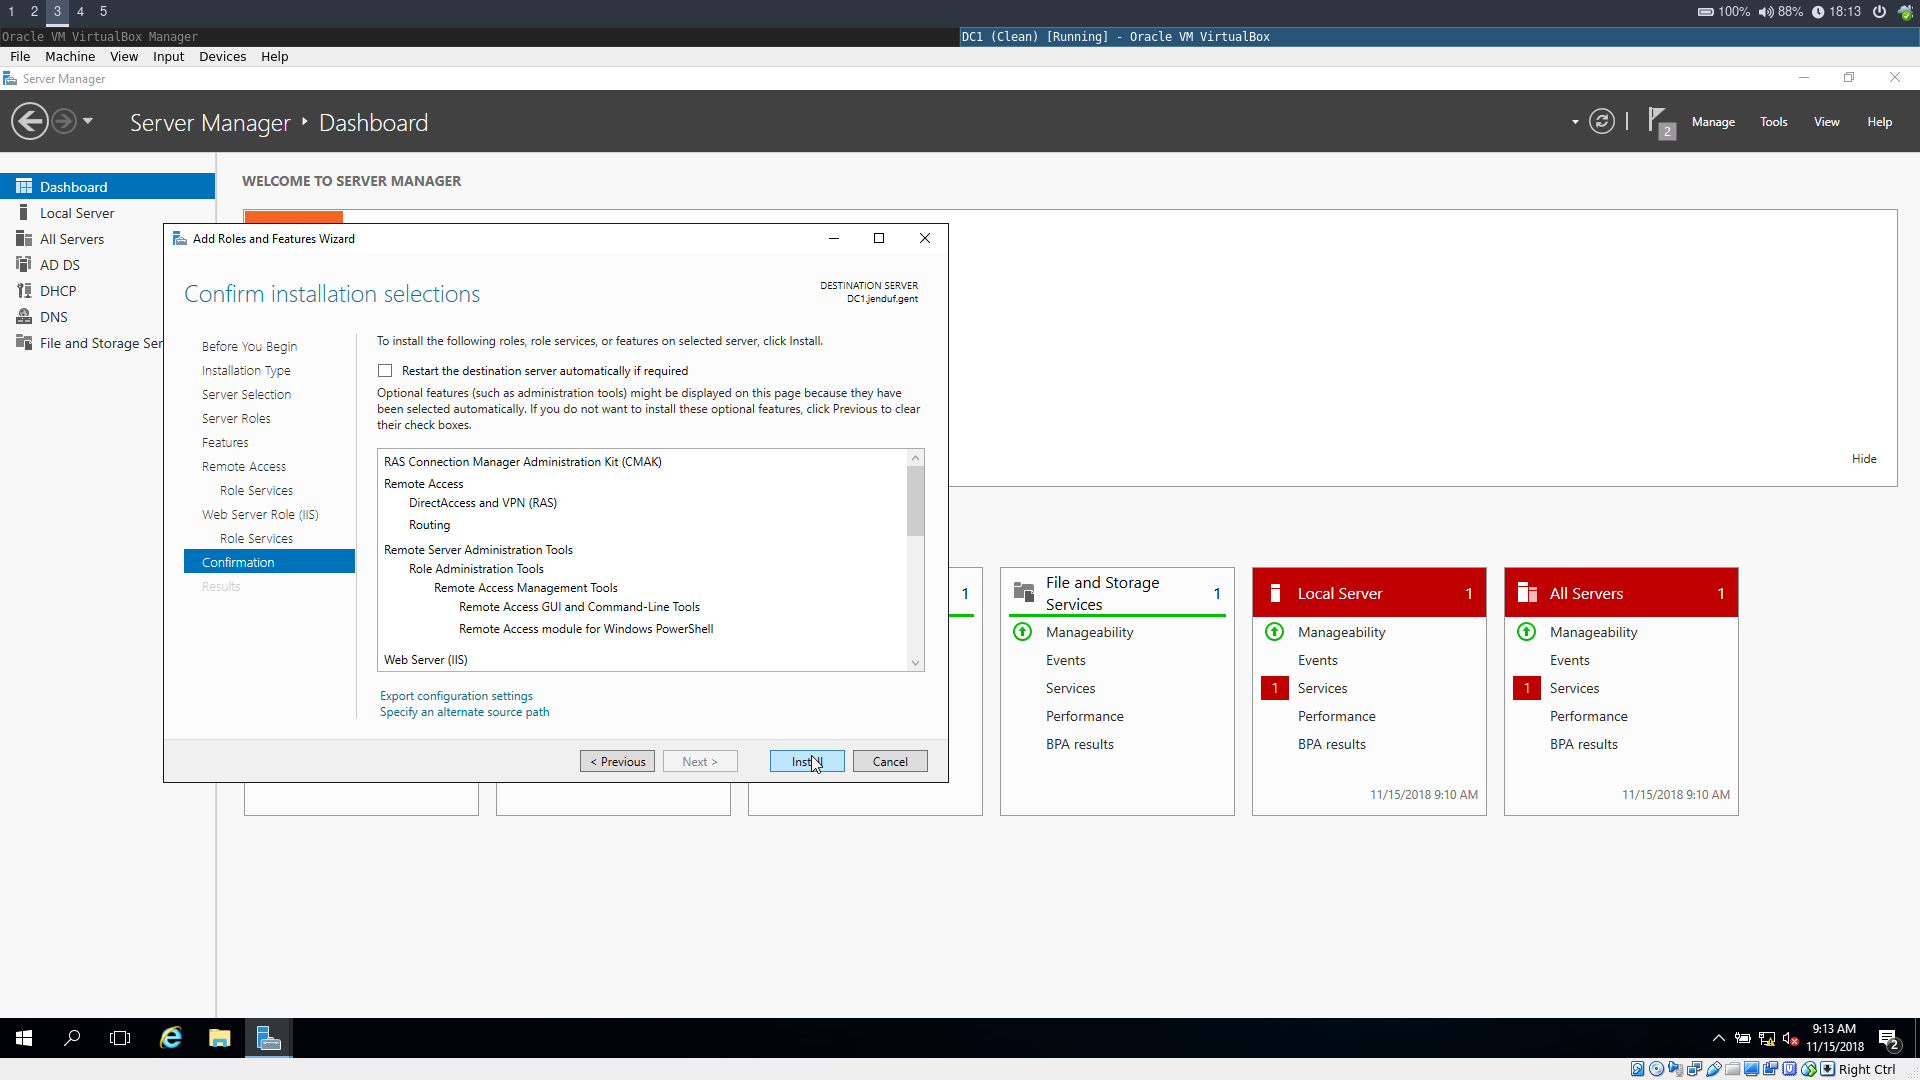
\includegraphics[width=15cm]{Pictures/DC1/Routing/1542302012.png}
	
	Volg de installatiewizard.
\end{center}
\begin{center}
	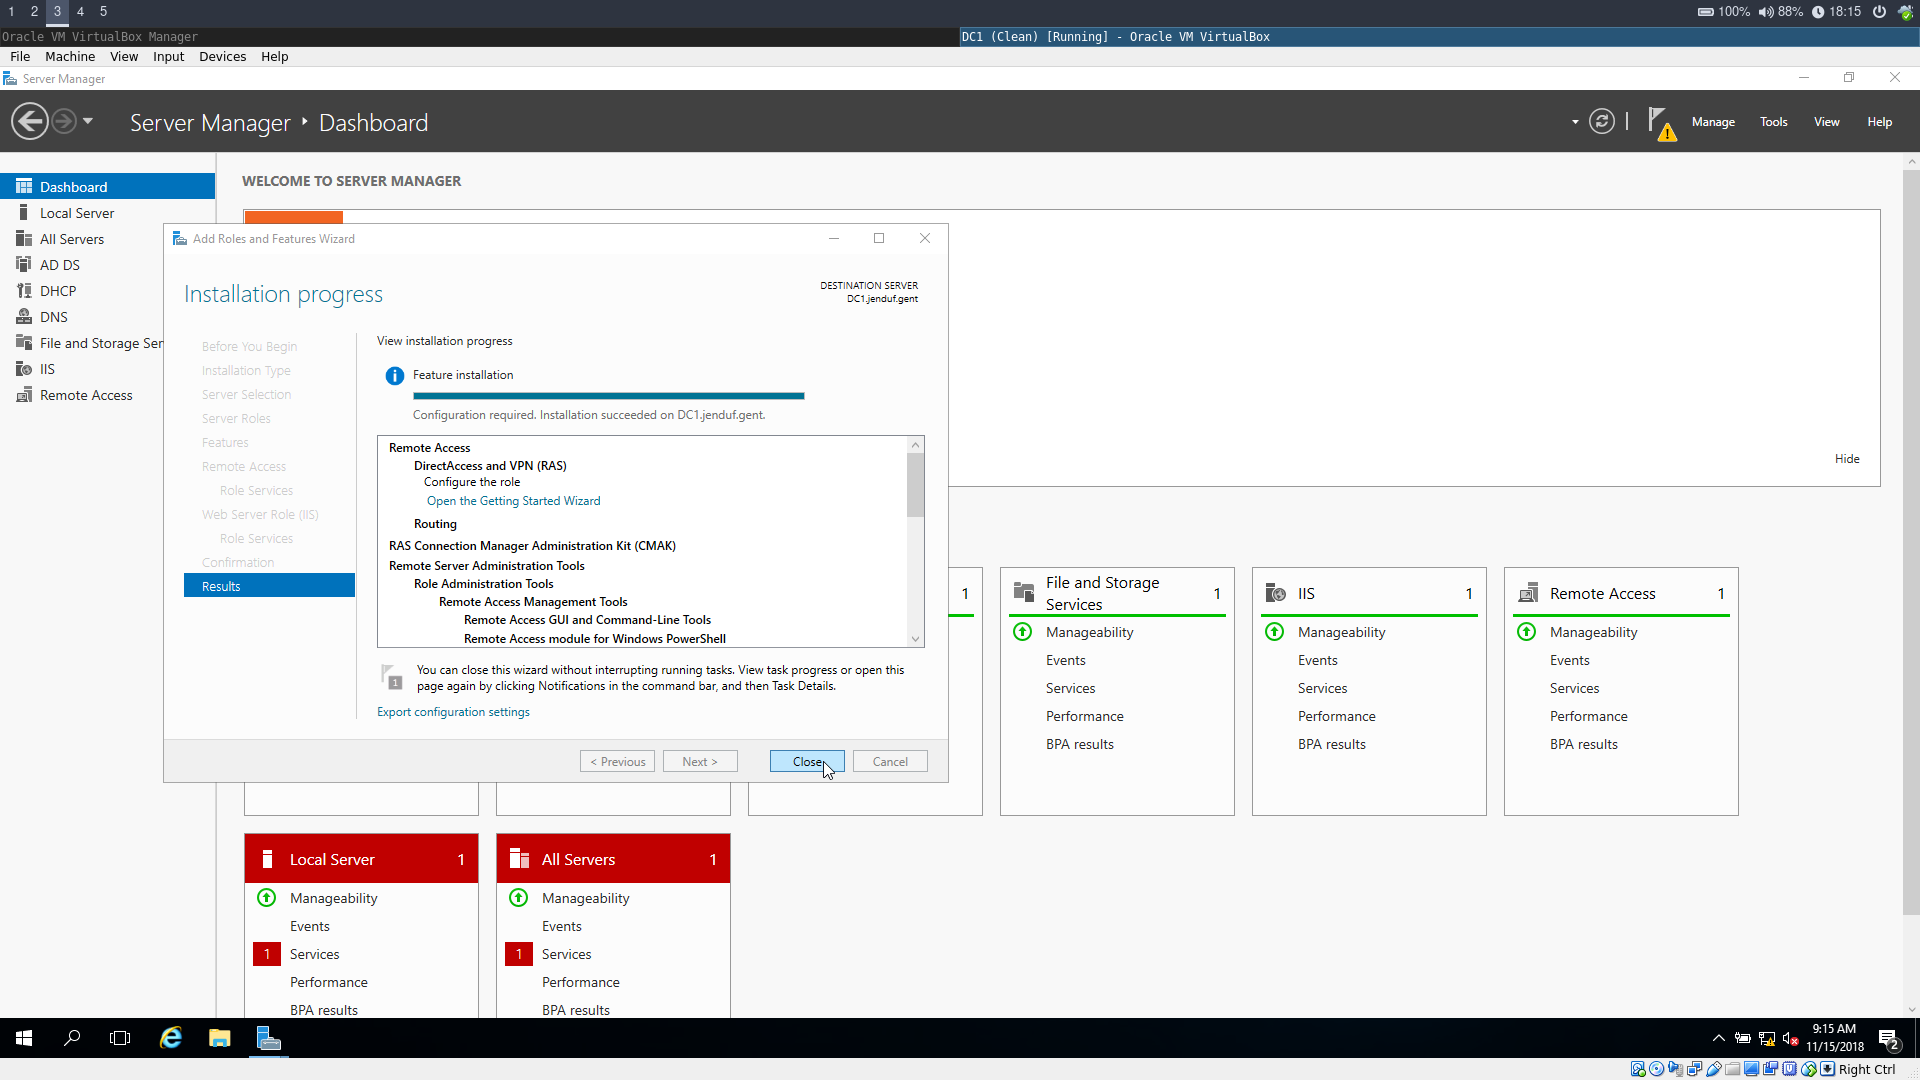
\includegraphics[width=15cm]{Pictures/DC1/Routing/1542302154.png}
\end{center}
\begin{center}
	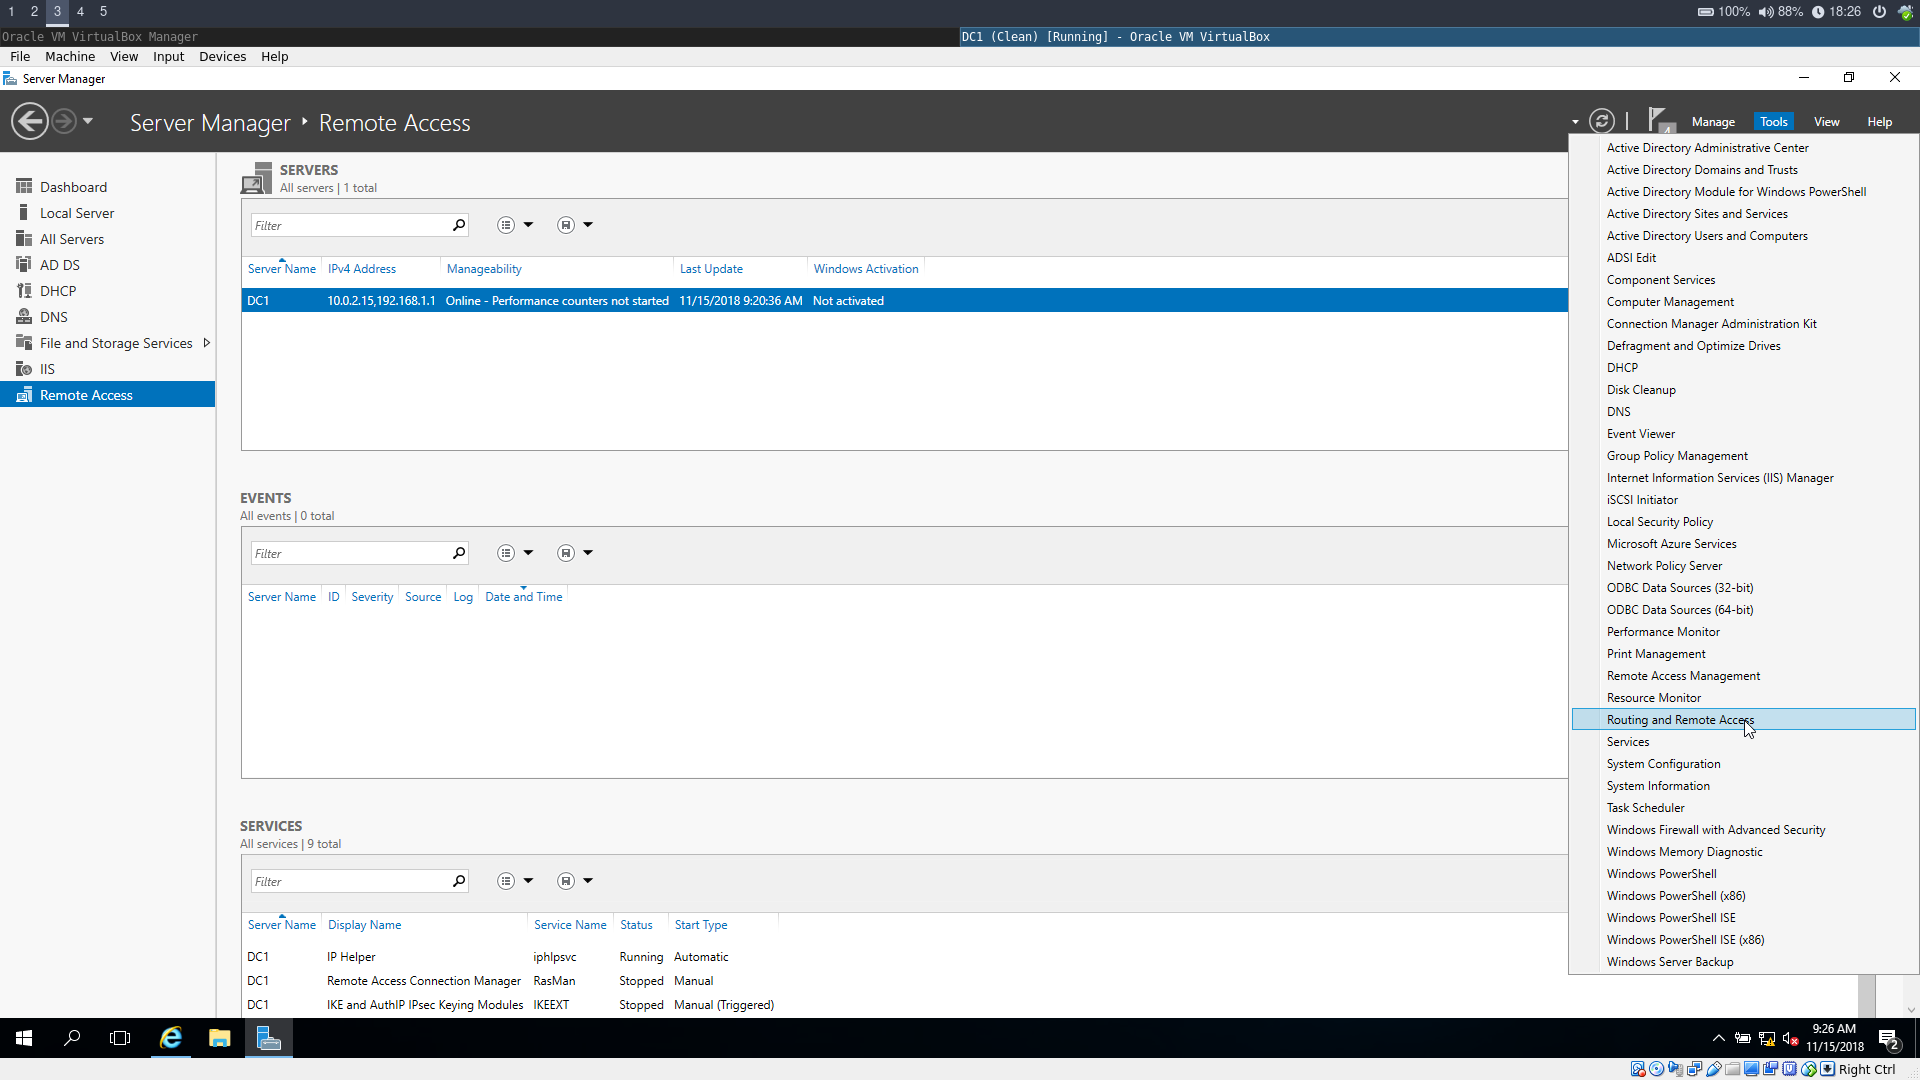
\includegraphics[width=15cm]{Pictures/DC1/Routing/1542302809.png}
	
	Ga naar "Routing and Remote Access".
\end{center}
\begin{center}
	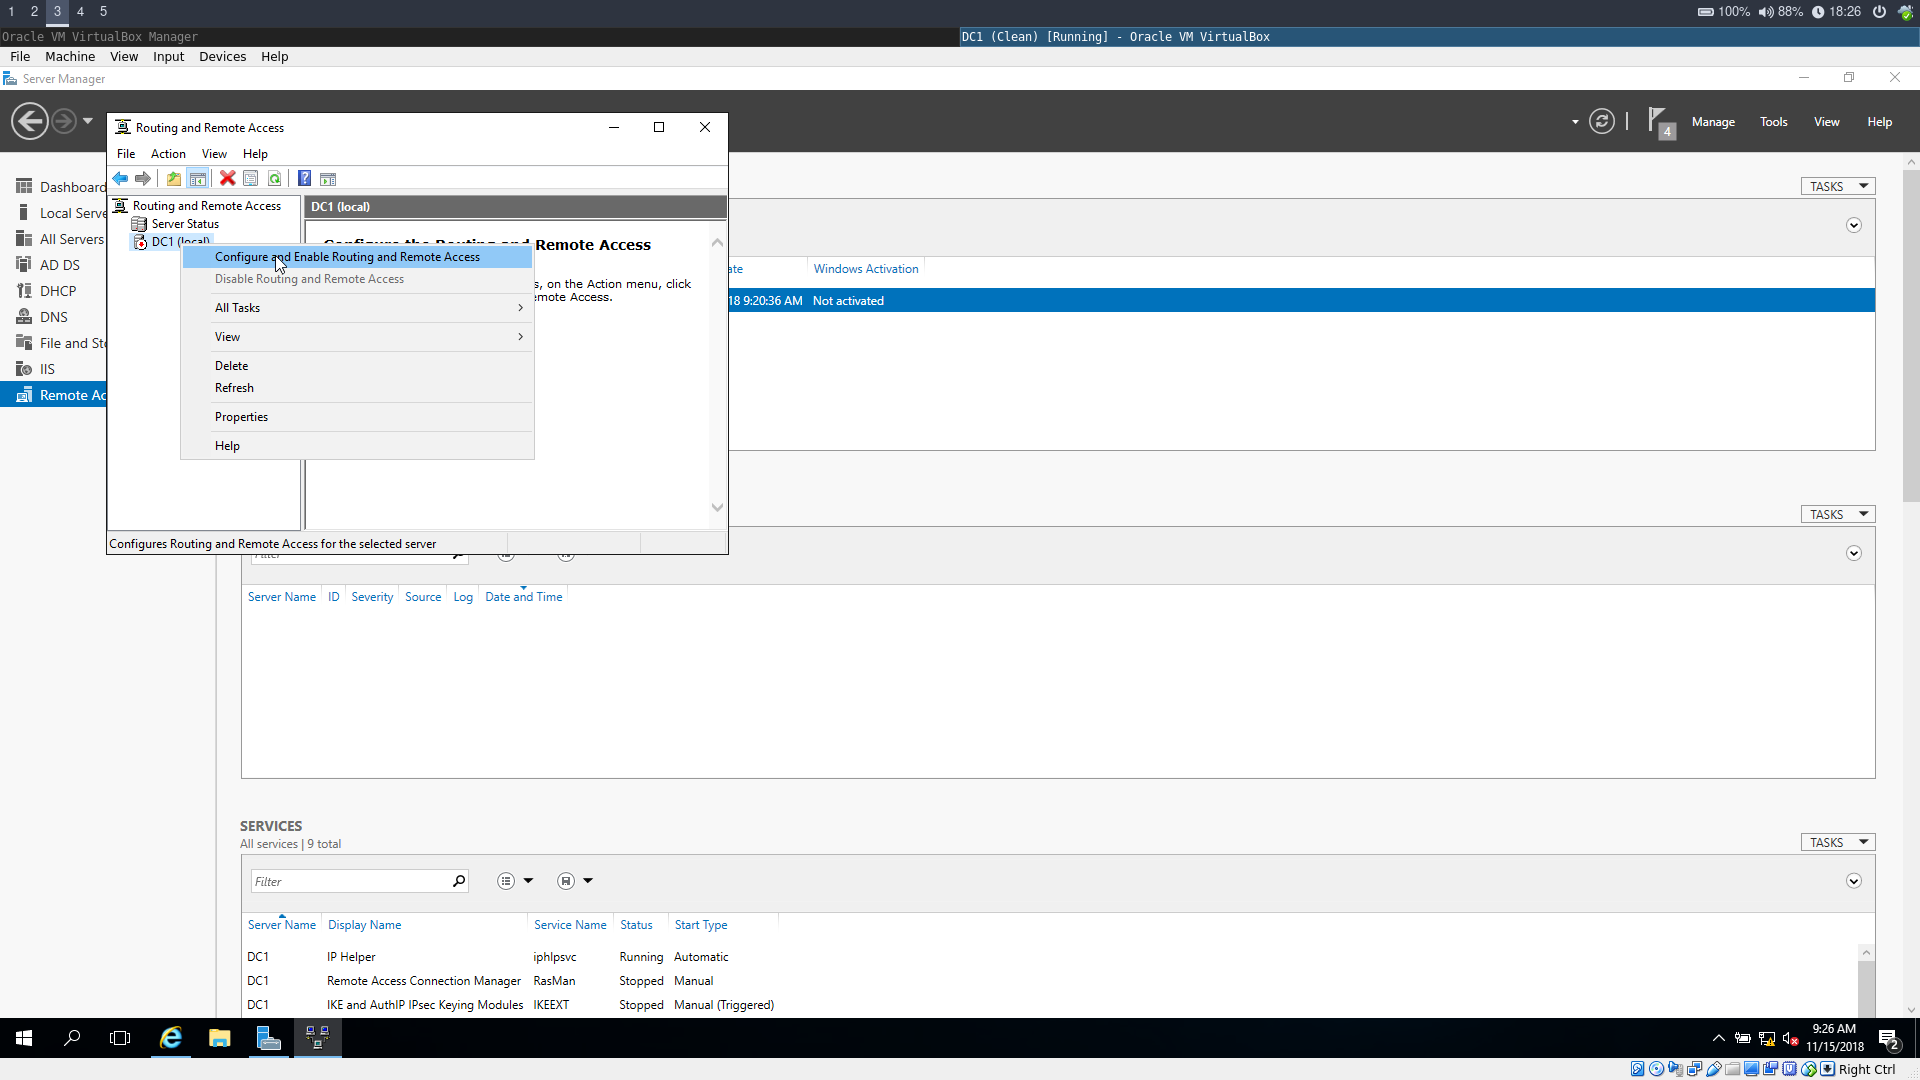
\includegraphics[width=15cm]{Pictures/DC1/Routing/1542302818.png}
	
	Selecteer met de rechtermuisklik de optie "Configure and Enable Routing and Remote Access"/
\end{center}
\begin{center}
	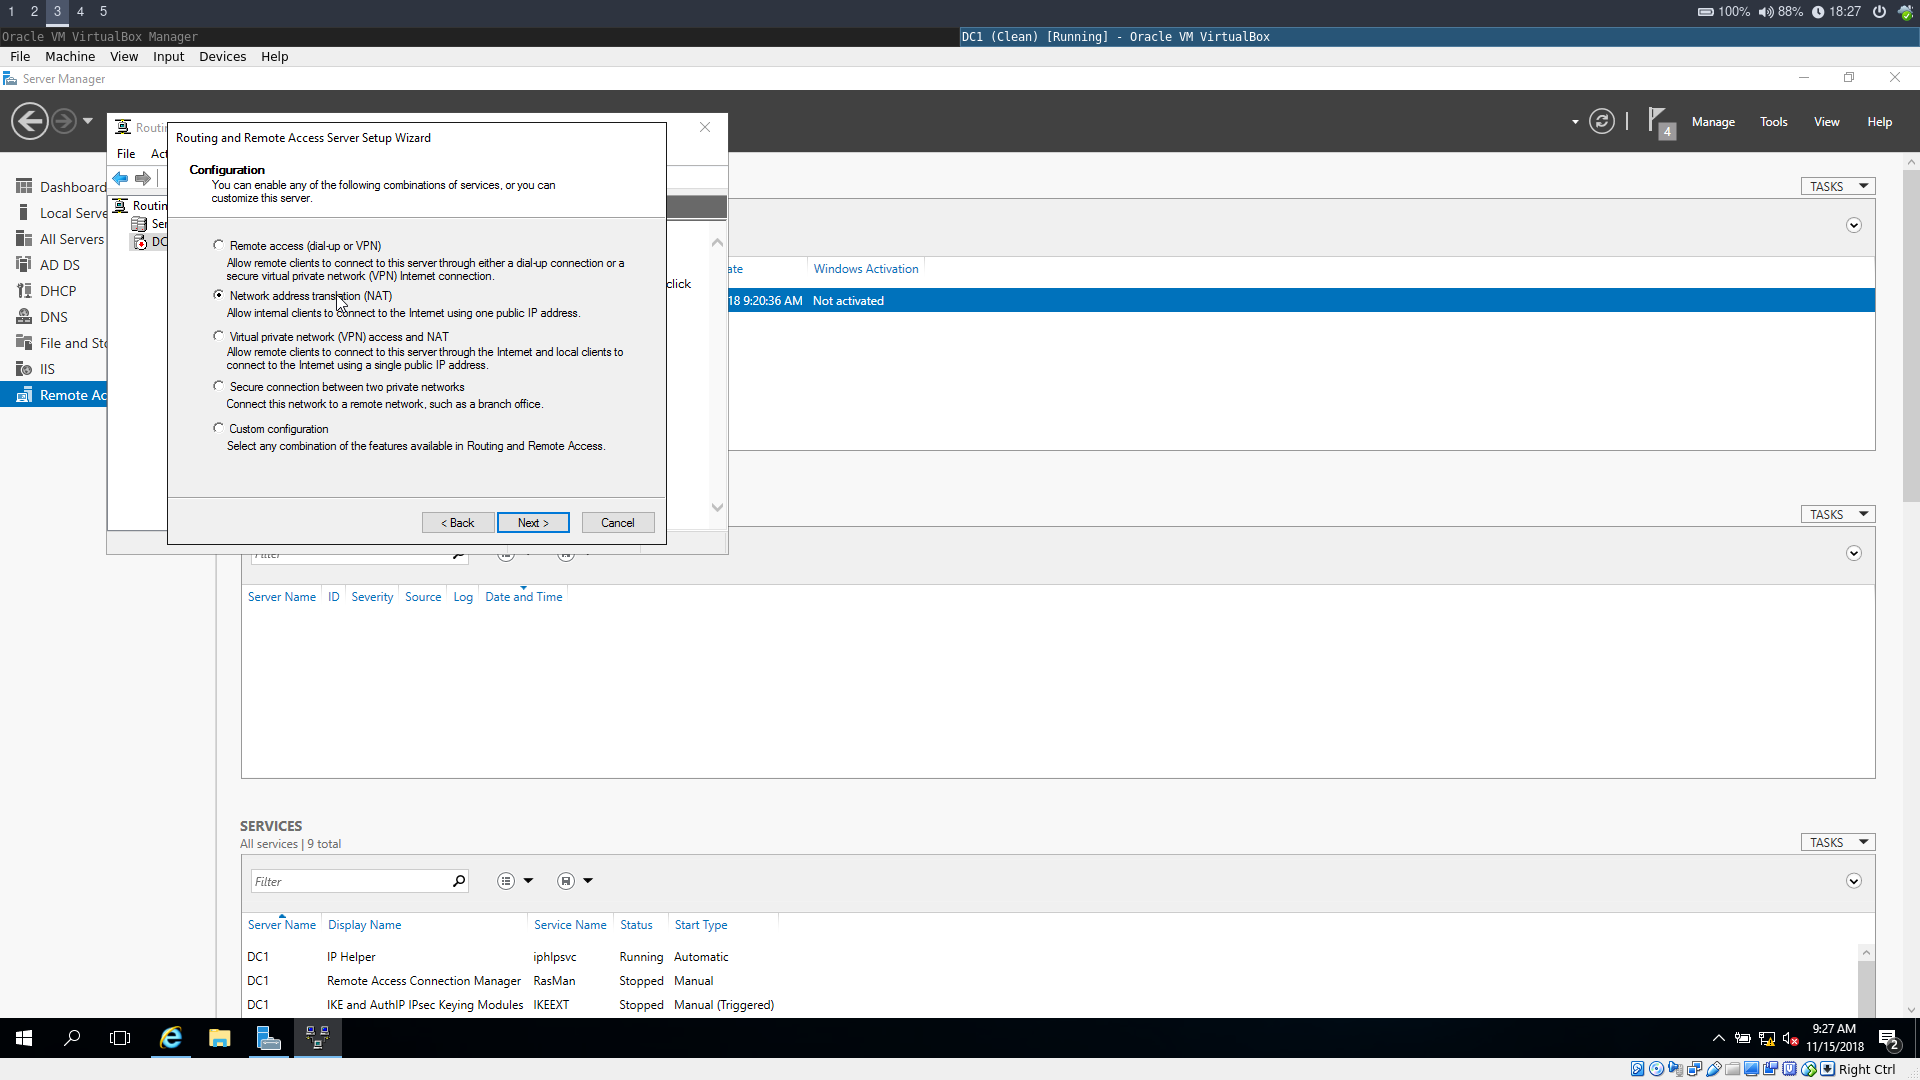
\includegraphics[width=15cm]{Pictures/DC1/Routing/1542302823.png}
	
	Selecteer "Network Address Translation".
\end{center}
\begin{center}
	\includegraphics[width=15cm]{Pictures/DC1/Routing/1542302956.png}
	
	Selecteer de adapter waarop DHCP geconfigureerd is.
\end{center}
\begin{center}
	\includegraphics[width=15cm]{Pictures/DC1/Routing/1542302960.png}
	
	Sluit de configuratiewizard af. Alle servers in het interne netwerk hebben nu internet via DC1.
\end{center}


\section{Powershell}
Script 1:
\begin{verbatim}
	#Activeer PS
	Set-ExecutionPolicy Unrestricted
	#Declaring variables
	$hostname = "ns1"
	
	#Computer naam wijzigen
	Rename-Computer -ComputerName $env:COMPUTERNAME -newName $hostname -Force -Restart
\end{verbatim}


Script 2:
\begin{verbatim}
	#Declaring variables
	$domainname = "jenduf.gent"
	
	#IP-adres en default gateway wijzigen
	New-NetIPAddress -InterfaceAlias "Ethernet" -IPAddress "192.168.1.1" 
	-PrefixLength 24 -DefaultGateway "192.168.1.1"
	
	#Firewall uitschakelen
	Set-NetFirewallProfile -Profile Domain,Public,Private -Enabled False
	
	#DC en DNS installeren en domeinnaam instellen
	Install-WindowsFeature AD-Domain-Services -IncludeManagementTools
	Install-ADDSForest -DomainName $domainname -SafeModeAdministratorPassword:
	(ConvertTo-SecureString -String "Admin2018" -AsPlainText -Force) -Force
	
	#Server opnieuw opstarten
	Restart-computer
\end{verbatim}
\end{document}